% GRUNDEINSTELLUNGEN -------------------------------------------

\documentclass[a4paper]{article}
\usepackage[ngerman]{babel}
\usepackage[utf8]{inputenc}


% EINGEBUNDENE PAKETE ------------------------------------------

\usepackage{pdfpages} % andere PDFs einbinden
\usepackage{verbatim} % program listings
\usepackage{latexsym} % Symbole zB Box
\usepackage{amssymb} % z.B. mathbb{}
\usepackage{amsmath} 
\usepackage{amsthm} % Für Lemmata, Sätze(Theoreme), Beweise (siehe unten)
\usepackage{tikz}	% Für Diagramme aus dem Programm Dia
\usepackage{makeidx} % fuer Stichwortverzeichnis
\usepackage{csquotes}
\usepackage{color}

% Verweise anklickbar machen
\usepackage{hyperref} % 1. 
\usepackage[figure]{hypcap} % 2. 


% EIGENE BEFEHLE -----------------------------------------------
% Bildbreite: Originalgröße oder falls größer als Seitenbreite/Spalte ==> skalieren
\makeatletter
\def\ScaleIfNeeded{%
\ifdim\Gin@nat@width>\linewidth
\linewidth
\else
\Gin@nat@width
\fi
}
\makeatother

% Neuer Befehl der Bilder standartisiert einbindet:
% includegraphicsdeluxe benötigt \ScaleIfNeeded und \ldate
% 1. innerhalb der figure-Umgebung mit dem Versuch, das Bild mittels [!htb] an genau dieser Position einzufügen
% 2. mit der Original- oder einer skalierten (mittels ScaleIfNeeded s.o.) Größe
% 3. mit einer Beschriftung (\caption{})
% 4. mit einem Label (\label{})
\newcommand{\includegraphicsdeluxe}[4]{
	\begin{figure}[!htb] 
	\centering
	\includegraphics[width=1\ScaleIfNeeded]{pics/\ldate_#1}
	\caption[#2]{#3}
	\label{#4}
	\end{figure}
}


% AND und OR Symbole
\newcommand{\und}{\wedge}
\newcommand{\oder}{\vee}

% Grundmengen
\newcommand{\N}{\mathbb{N}}
\newcommand{\Z}{\mathbb{Z}}
\newcommand{\Q}{\mathbb{Q}}
\newcommand{\R}{\mathbb{R}}
\newcommand{\C}{\mathbb{C}}

% größenangepasste Betragsstriche, Klammern, ...
\newcommand{\abs}[1]{\ensuremath{ \left\vert #1 \right\vert }}
\newcommand{\rbr}[1]{\ensuremath{ \left( #1 \right) }} % round brackets ()
\newcommand{\cbr}[1]{\ensuremath{ \left\lbrace #1 \right\rbrace }} % curly brackets {}
\newcommand{\sbr}[1]{\ensuremath{ \left[ #1 \right] }} % square brackets []

% griechische Buchstaben
\newcommand{\oiO}{\omega\in\Omega}

% Vektoren mit Klammern und so 
\newcommand{\vektor}[1]{\ensuremath{ \rbr{ \begin{array}{c} #1 \end{array} } }} 

% Datum der einzelnen Lektionen definieren
\newcommand{\ldate}{2015-10-01}	% define lessiondate

% Anmerkung Professor
\newcommand{\profnote}[1]{\marginpar{\tiny{\textquote{#1}}}}

% lokale Platzhalter
\newcommand{\locpl}{}

% Dokumenteneigenschaften
\newcommand{\pTitle}{Wahrscheinlichkeitstheorie und Statistik}
\newcommand{\pShortName}{M. Zell}
\newcommand{\pSemester}{WS 2015/16}
\newcommand{\pProfessor}{Prof. Dr. Josef Hörwick}

% EINRÜCKUNG ---------------------------------------------------
\setlength{\parindent}{0pt} % Erste Zeile in Absätzen nicht einrücken.

% KOPF- UND FUSSZEILE ------------------------------------------
\usepackage{fancyhdr}
\pagestyle{fancy}
\fancyhf{}
 
%Kopfzeile mittig mit Kaptilname
\fancyhead[L]{\textsf{\nouppercase{\leftmark}}}
\fancyhead[R]{\textsf{\thepage}}
%Linie oben
\renewcommand{\headrulewidth}{0.5pt}
%Fußzeile 
\fancyfoot[L]{\tiny{\pTitle}}
\fancyfoot[R]{\tiny{\pShortName, \pSemester, \ldate}}
%Linie unten
\renewcommand{\footrulewidth}{0.5pt}
 
% START DES EIGENTLICHEN DOKUMENTS -----------------------------
\author{\pShortName}
\title{Mitschrift\\\pTitle, \pSemester\\\pProfessor}

% Stichwortverzeichnis erstellen
\makeindex

\begin{document}
\maketitle
\newpage
\tableofcontents
\newpage
\listoffigures

% Sätze usw. aus asmthm
\newtheorem{satz}{Satz}[section] 
\newtheorem{defi}{Definition}[section] 
\newtheorem{lem}{Lemma}[section] 
\newtheorem{beh}{Behauptung}[section] 

% einzelne Kapitel
\renewcommand{\ldate}{2015-10-01}

\section{Hinweise}
Diese Mitschrift basiert auf der Vorlesung \textquote{\pTitle} von \pProfessor \ im \pSemester. Du kannst sie gerne benutzen, kopieren und an andere weitergeben. Auch in der Prüfung - soweit zugelassen \footnote{\url{http://www.cs.hm.edu/meinstudium/studierenden_services/fi_pruefungskatalog.de.html}} - kannst du sie gerne als Hilfsmittel verwenden, wenn das meine Nutzung als Prüfungshilfsmittel nicht in irgendeiner Weise beeinträchtigt.\\

Natürlich besteht kein Anspruch auf Aktualität, Richtigkeit, Fortsetzung meines Angebots oder dergleichen. Sollten dir Fehler auffallen oder solltest du Verbesserungsvorschläge haben, würde ich mich über eine E-Mail (zell@hm.edu) freuen. Wenn du mir als kleines Dankeschön z.B. ein Club-Mate\footnote{\url{http://www.clubmate.de/ueber-club-mate.html}} ausgeben möchtest, findest du mich meistens hier: \url{http://fi.cs.hm.edu/fi/rest/public/timetable/group/if3b}. Wenn nicht, ist es auch ok ;-)\\

Nach der Prüfung werde ich den \LaTeX-Quelltext veröffentlichen, damit die Mitschrift weitergeführt, korrigiert und ergänzt werden kann.\\

Viele Grüße\\
\pShortName
% Vorlesung vom 05.10.2015
\renewcommand{\ldate}{2015-10-05}

\section{Allgemeines}

\begin{itemize}
\item kein Skript. Alles wichtige steht an der Tafel.
\item Literatur: Norbert Henze, Stochastik für Einsteiger, Vieweg/Teubner
\item keine Hausaufgaben
\item Übungsaufgaben gibt es immer zwischendurch und alte Prüfungsaufgaben gegen Ende des Semesters
\end{itemize}

\section{Zufallsexperimente}

Experimente: Würfeln, Ergebnismenge $ \Omega = \{1,2,3,4,5,6\}$, Münze werfen: $ \Omega = \{K, Z\}$. Solange würfeln bis eine 6 kommt: $ \Omega = \{ 1,2,3,4,...\} = \N $\\
\profnote{Man kann mehrere Exerimente auch zusammenfassen}n Einzelexperimente $ \Rightarrow $ Kartesisches Produkt: $ \Omega_1, \Omega_2, ...,  \Omega_n, \Omega = \Omega_1 \times \Omega_2 \times ... \times  \Omega_n $\\
Zum Beispiel erst würfeln, dann Münze: \\
$ \Omega_1 = \{1,...,6\}, \Omega_2=\{K,Z\} \Rightarrow \Omega=\{(a,b) | a\in \Omega_1, b\in \Omega_2\}$\\
Zweimal nacheinander würfeln: $ \underbrace{\Omega}_{1. Wurf}=\{(\underbrace{a}_{1.},\underbrace{b}_{2. Wurf}) : 1 \leq a,b \leq 6 \} $\\

Mit rotem und grünen Würfel gleichzeitig: $ \Omega = \{(\underbrace{a}_{gr"uner}, \underbrace{b}_{roter}) | 1\leq a,b\leq 6\} $\\
In einer Urne sind die Kugeln 1 bis n. Es wird k mal mit Rücklegen gezogen: $ \Omega = \{(\underbrace{a_1}_{1. Zug}, \underbrace{a_2}_{2. Zug}, ..., a_k) | 1\leq a_i \leq n \}$

In einer Schachtel mit den Kugeln 1, 2, 3, 4 werden zwei mit einem Griff gezogen. Wie sieht $ \Omega $ aus?\\
$ \Omega=\{\{a_1,a_2\} | a_1 \neq a_2, 1\leq a_1,a_2\leq 4\} $\\
$ \Omega=\{\{a_1,a_2\} | 1\leq a_1, a_2\leq 4, a_1 < a_2 \} $\\

Lotto: 6 Kugeln aus 49: $ \Omega=\{(\underbrace{a_1}_{1. Kugel}, \underbrace{a_2}_{2. Kugel}, a_3, a_4, a_5, a_6) | a_i \textrm{sind verschieden} \}$ (mit Reihenfolge)\\
$ \Omega=\{(a_1,...,a_6) | a_1 < a_2 < a_3 < a_4 < a_5 < a_6\}$ (ohne Reihenfolge)\\

\subsection{2. Ereignisse}
$ A \subset \Omega$ heißt Ereignis, Ergebnis $ \omega $. A ist eingetreten, wenn $\omega \in A$. \\
$\{\omega\} $: Elementarereignis\\
$ \Omega $: sicheres Ereignis\\
$\emptyset $: unmögliches Ereignis\\
$A \cap B$: A und B sind eingetreten.\\
$A\cup B$: A oder B\\
$A_1\cap A_2\cap ... \cap A_n$\\
$A_1\cup A_2\cup ... \cup A_n$\\
$B \setminus A= \{\omega \in B : \omega \notin A \} $: B minus A. \\
Gegenseitiges Komplement: $ \overline{A} = \Omega \setminus A = \{\omega : \omega \notin A \}$\\
A, B heißen disjunkt, wenn $ A \cap B = \emptyset $. Für $ A \cup B $ schreibt man dann $A+B$.\\

\subsection{Zweimal Würfeln}
A: erster Wurf 5 $\Rightarrow A=\{(5,1),(5,2),...(5,6)\}$\\
B: zweiter Wurf höher als erster 
$\Rightarrow B = \{ (1,2), (1,3), (1,4), (1,5), (1,6), (2,3), (2,4), $
$(2,5), (2,6), (3,4), (3,5), (3,6), (4,5), (4,6), (5,6) \} $

\subsection{Rechenregeln in der Mengenlehre}
Kommutativ: $ A\cap B = B\cap A $ und $ A\cup B = B\cup A $\\
Assoziativ: $ A\cap (B\cap C) = (A\cap B) \cap C$ und $ A\cup (B\cup C) = (A\cup B) \cup C$ \\
De Morgan: $ \overline{(A\cup B)} = \bar{A}\cap \bar{B} $ und $ \overline{(A\cap B)} = \bar{A} \cup \bar{B}$, Beispiel: $ |A\cup B| = |A|+|B|-|A\cap B|$ \\
Distributiv: $ A \cap (B\cup C) = (A\cap B)\cup (A\cap C)$ und $ \underbrace{A\cup (B\cap C)}_{L} = \underbrace{(A\cup B) \cap (A\cup C)}_{R}$

\paragraph{Beweis $ L = R $}
\begin{enumerate}
\item $x \in L \Rightarrow x\in R \Rightarrow L \subset R $
\item $x \in R \Rightarrow x\in L \Rightarrow R \subset L $
\end{enumerate}
$\Rightarrow R=L \Box$\\

\subsection{Zufallsvariable}

Abbildung: $ X: \Omega \rightarrow \R$ heißt Zufallsvariable, z.B. zweimal würfeln. X ist die Augensumme: $ X(\omega_1, \omega_2) = \omega_1+\omega_2$\\
$ X_1$: erste Augenzahl\\
$ X_2$: zweite Augenzahl\\
$X = X_1+X_2$\\
$(X_1 + X_2)(\omega) = X_1(\omega) + X_2(\omega) = \omega_1 + \omega_2$\\

\paragraph{Abkürzungen}
$ \{X=K\} = \{\omega\in\Omega | X(\omega) = K\}$\\
Augensumme mindestens 10: $ \{X \geq 10\} $\\
Augensumme zwischen 3 und 8: $ \{3 \leq X \leq 8\}$\\
Wertebereich von $X$ ist $X(\Omega) = \{ X(\omega) : \omega \in \Omega \} $ \\
Arithmetik mit Zufallsvariable (ZV): \\
$ (X\cdot Y)(\omega) = X(\omega) \cdot Y(\omega)$\\
$ (a \cdot X)(\omega) = a \cdot X(\omega)$\\
$ \{X\leq Y\} = \{\omega\in\Omega | X(\omega) \leq Y(\omega) \}$\\
 
\subsection{Indikatorfunktionen}
$ I_{A}(\omega) = $ 1, falls $ \omega\in A $, sonst 0 ($A\in \Omega$). Die Indikatorfunktion I zeigt an, ob das Ereignis eingetreten ist oder nicht. \\
$ I_{A\cap B} = I_A \cdot I_B $\\
$ I_A = I\{A\} $ sind mögliche Schreibweisen im Buch.\\ 
$ I_{A_1\cap A_2\cap ... \cap A_n} = I_{A_1}\cdot I_{A_2}\cdot ... \cdot I_{A_n} $\\
$ I_{\bar{A}} = 1 - I_A $\\
$ I_A = I_A \cdot I_A$

\subsection{Zählvariable}

$ A_1, ..., A_n $ Ereignisse: $ X=I_{A_1} + I_{A_2} + ... + I_{A_n} $. X zählt, wie viele Ereignisse $A_1, ..., A_n$ eingetreten sind. \\
$ X(\omega) = $ Anzahl der $A_i$, in denen $\omega$ liegt. $ \{X=n\} = A_1\cap A_2\cap ...\cap A_n$ und $ \{X=0\} = \bar{A_1} \cap \bar{A_2} \cap ... \cap \bar{A_n} $

\paragraph{Beispiel:} Ein Treffer-Niete-Experiment wird n-mal wiederholt.\profnote{Treffer=1, Niete=0} \\
$ \Omega=\{(a_1,a_2,...,a_n) : a_i=1/0 \} $\\
$ A_j = \{\omega : \omega_j=1\} $ in j-ten Versuch Treffer\\
$ X=I_{A_1} + I_{A_2} + ... + I_{A_n} $ zählt Anzahl der Treffer\\
$ X(\omega) = X(\omega_1, \omega_2, ..., \omega_n) = \omega_1 + \omega_2 + ... + \omega_n $

\paragraph{Übung 3.5 (Buch)}
$ \Omega = \{ ( \omega_1, \omega_2, \omega_3 ) | 1 \leq \omega_i \leq 6 \} $\\
$ X: \Omega \rightarrow \R $\\
$ (\omega_1, \omega_2, \omega_3) \rightarrow $ 100, wenn $\omega_1=6$\\
$ (\omega_1, \omega_2, \omega_3) \rightarrow $ 50, falls $\omega_2=6$ und $\omega_1 \neq 6$\\
$ (\omega_1, \omega_2, \omega_3) \rightarrow $ 10, falls $\omega_2 = 6$ und $\omega_a, \omega_2\neq 6$\\
$ (\omega_1, \omega_2, \omega_3) \rightarrow $ -30, falls $\omega_1, \omega_2, \omega_3\neq 6$\\

% Vorlesung vom 06.10.2015
\renewcommand{\ldate}{2015-10-06}

\section{Relative Häufigkeit}\index{Häufigkeit!relative}

\subsection{Relative Häufigkeit am Beispiel des Reißnagelversuchs}\index{Reißnagelversuch}
Ein Reißnagel wurde 300 mal geworfen. Er kann grundsätzlich in den zwei Positionen 1 und 0 landen (Abb. \ref{fig:reissnagelversuch1}). Die absoluten Häufigkeiten sind: 1 kommt 124 mal, 0 kommt 176 mal vor. Die relative Häufigkeit von 1 beträgt $ \frac{124}{300}=0.413=41,3\% $, die von 0 beträgt $ \frac{176}{300}=0.586=58,6\% $.

\includegraphicsdeluxe{reissnagelversuch1.jpg}{Reißnagelversuch}{Der Reißnagel kann auf seinem Kopf landen (1) oder eben nicht (0)}{fig:reissnagelversuch1}

\subsection{Relative Häufigkeit allgemein}
Einzelexperiment mit Ergebnismenge $ \Omega $ wird n mal wiederholt. Dadurch entsteht ein Datenvektor\index{Datenvektor} $ (\omega_1, \omega_2, ..., \omega_n), \omega_i \in \Omega $. \profnote{Dieser Datenvektor steht fest und kann nachträglich nicht mehr geändert werden.} Jedem Ereignis A von $ \Omega $ können wir eine relative Häufigkeit zuordnen: $ r(A) = |\{ j : 1\leq j\leq n \textrm{ und } \omega_j \in A \}| \cdot \frac{1}{n} $. 
\profnote{Die relative Häufigkeit von A $ \approx $ Wahrscheinlichkeit von A.}

Für diese relative Häufigkeit gilt: 
\begin{enumerate}
\item $ 0\leq r(A)\leq 1 $
\item $ r(\Omega) = 1 $
\item $ r(A+B) = r(A) + r(B) $
\end{enumerate}

\subsection{Beispiel}
$ \Omega = \{ 1,2,3,4,5,6 \}, n=10, \textrm{Datenvektor: } (5,1,1,6,2,3,4,2,1,5), \textrm{Ereignisse: } A=\{ 1,2 \}, B=\{ 3,4 \}, A\cap B=\emptyset $\\
$ r(A) = 5 \cdot \frac{1}{10} = \frac{5}{10} $ und $ r(B)=2\cdot \frac{1}{10}=\frac{2}{10} $\\
$ r(A\cup B) = \frac{7}{10} $

\subsection{Stabilisierung}\index{Stabilisierung}
Angenommen Datenvektor sehr lang ($ n = 10 000 $), Ereignis $A \subset \Omega $. Man berechnet die $ r_k(A) $ indem man die ersten k Daten berücksichtigt, also: $ r_{10}(A), r_{11}(A), r_{12}(A), ..., r_{10 000}(A) $ \\
$ r_k(A) = | \{ j : 1\leq j \leq k \textrm{ und } \omega_j \in A \} | \cdot \frac{1}{k} $

\includegraphicsdeluxe{stabilisierung.jpg}{Stabilisierung}{Das Diagramm zeigt beispielhaft, was unter Stabilisierung gemeint ist.}{fig:}

\subsection{Empirisches Gesetz}\index{Empirisches Gesetz}
Von der Stabilisierung der relativen Häufigkeit von A. Für $ k\rightarrow \infty $ läuft $r_k(A) $ gegen einen festen Wert $ P(A) $.

\subsection{Übung 4.2 (Buch)} Lotto 6 aus 49.
Die ersten 2058 Ziehungen enthielten 198 mal die 13 und 248 mal die 43 ($ \Omega=\{(a_1 < a_2 < a_3 < a_4 < a_5 < a_6) : 1\leq a_i\leq 49 \} $). Der Datenvektor hat die Länge $ n = 2058 $. \\
$ A_{13}: $ "13 wird gezogen", $ r(A_{13}) = \frac{198}{2058} = 0.096 $\\
$ A_{43}: $ "43 wird gezogen", $ r(A_{43}) = \frac{248}{2058} = 0.120 $\\
Wie groß ist die relative Häufigkeit einer Zahl, wenn jede Zahl gleich oft gezogen wird?\\
Gezogene Kugeln: $ 6 \cdot 2058 $\\
Jede gleich oft: $ \frac{6\cdot 2058}{49}=252 \Rightarrow r_(A_k)=\frac{252}{2058}=\frac{6}{49} $

\section{Deskriptive Statistik}\index{Statistik!deskriptive}

\subsection{Stabdiagramm}\index{Stabdiagramm}
\profnote{Beispiel aus dem Buch (Seite 24)}Bundestagswahl mit $ n = 43 371 190 $ gültigen Zweitstimmen. Dabei entsteht das folgende Stabdiagramm (Abb. \ref{fig:stabdiagramm1}).

\includegraphicsdeluxe{stabdiagramm1.png}{Stabdiagramm Stimmenverteilung}{Aufteilung der Parteien in $ \% $ (Quelle: Buch)}{fig:stabdiagramm1}

\subsection{Histogramm}\index{Histogramm}
Bei 1000 Glühbirnen wurde die Lebensdauer getestet.\\ % \profnote{Die Glühbirnen sind ja jetzt verboten. Ich habe im Internet auch einen ganzen Karton bestellt.}
\begin{tabular}{|c|c|c|c|c|}
\hline Stunden & ausgefallene Glühbirnen & relative Häufigkeit & Höhe \\ 
\hline 0-50 & 20 & 0.02 & 0.0004 \\ 
\hline 50-200 & 80 & 0.08 & 0.00053 \\ 
\hline 200-400 & 120 & 0.12 & 0.0006 \\ 
\hline 400-600 & 180 & 0.18 & 0.0009 \\ 
\hline 600-800 & 500 & 0.5 & 0.0025 \\ 
\hline 800-1000 & 100 & 0.1 & 0.0005 \\ 
\hline 
\end{tabular} 

\includegraphicsdeluxe{histogramm1.jpg}{Beispiel für ein Histogramm}{Rechteckfläche $ = $ relative Häufigkeit, Höhe $ \times $ Breite $ = $ relative Häufigkeit, Höhe $ = \frac{\textrm{relative Häufigkeit}}{\textrm{Breite}} $ }{fig:histogramm1}

\subsection{Lagemaße}
$ x_1, ..., x_n $ Zahlen. Suche Zahl l für die "grobe Lage".\\
Forderung: $ l(x_1+a, x_2+a, ..., x_n+a) = l(x_1, ..., x_n) + a $\\
arithmetisches Mittel: $ \overline{x} = \frac{1}{n}(x_1+x_2+...+x_n) $ Forderung erfüllt!

\paragraph{Aufgabe} Für welches $t\in \R$ ist $ \sum_{i=1}^{n}(x_i-t)^2 $ minimal? Für $t=\overline{x}$! Wegen: $ f(t)=\sum_{i=1}^{n}(x_i-t)^2 $\\
$ f'(t) = -\sum_{i=1}^{n}2(x_i-t) = 0 $\\
$ \sum_{i=1}^{n}(x_i-t) = 0 $\\
$ \sum_{i=1}^{n} x_i = n\cdot t $\\
$ t = \frac{\sum_{i=1}^{n}x_i}{n} = \overline{x} $

\subsection{Gewichtetes Mittel}
\begin{tabular}{|c|c|c|c|c|}
\hline Werte & $ a_1 $ & $ a_2 $ & ... & $ a_n $ \\ 
\hline Gewichte & $ g_1 $ & $ g_2 $ & ... & $ g_n $ \\ 
\hline 
\end{tabular} 
$ \overline{x} = \frac{\sum_{i=1}^{n}g_i a_i}{\sum_{i=1}^{n} g_i} $

\paragraph{Beispiel Schulnoten}
Noten: 2,4,6,3,4,2,5\\
Gewicht: 1,5,1,3,3,5,1\\
Endnote $= \frac{1\cdot 2+ 5\cdot 4 + 1\cdot 6+ 3\cdot 3 + 3\cdot 4+ 5\cdot 2 + 1\cdot 5}{1+5+1+3+3+5+1} = 3.37 $

% \profnote{Hoffentlich bekommt die Deutschlehrerin das mit den gewichteten Noten hin. Eventuell muss sie die Mathelehrerin fragen. Und für die schriftliche Bewertung fragt dann die Mathe- die Deutschlehrerin.}
% Vorlesung vom 12.10.2015
\renewcommand{\ldate}{2015-10-12}

\subsection{Der empirische Median}
Die Stichprobe ist der Größe nach sortiert, also $ x_1 \leq x_2 \leq ... \leq x_n $. Der Median $ x_{\frac{1}{2}} = x_{0.5} = x_{50 \%} = x_{ \frac{n+1}{2}} $, falls ungerade und $ x_{0.5} = \frac{1}{2} (x_{\frac{n}{2}} + x_{\frac{n}{2}+1}) $

\subsubsection{Beispiel}
\begin{enumerate}
\item $ 3,4,5,6,7 \Rightarrow x_{0.5} = 5 $
\item $ 3,4,5,6,7,8 \Rightarrow x_{0.5} = 5.5 $
\item $ 3,3,4,5,6,20 \Rightarrow x_{0.5} = 4.5 $; vgl. dazu das arithmetische Mittel: $ \overline{x} = \frac{3+3+4+5+6+20}{6} = 6.8 $
\end{enumerate}

Der Median unempfindlich gegen Ausreißer, das arithmetische Mittel nicht. 

Minimiere $ \sum_{j=1}^{n} | x_j - t | $. Bei welchem t minimal? Beim Median: 3 3 4 $ \vert $ 5 6 7 % \profnote{Mitdenken! Nicht, dass ich einen Unsinn erzähl.}

\subsubsection{Verallgemeinerung}
Für den Median $ x_{0.5} $ gilt: \profnote{Links und rechts vom Median sind gleich viele Werte.}
\begin{itemize}
\item Mindestens 50\% der Werte sind $\leq x_{0.5} $
\item Mindestens 50\% der Werte sind $\geq x_{0.5} $
\end{itemize}

Der p Quantil $ x_p $
\begin{itemize}
\item Mindestens $p \cdot 100\%$ der Werte sind $\leq x_p $
\item Mindestens $100\% - p \cdot 100\% $ der Werte sind $\geq x_p $
\end{itemize}

\subsection{Streuungsmaße}
$ \sigma $ Streuungsmaß\\
Formel: $ \sigma(x_1,...,x_n) = \sigma(a+x_y,a+x_2,...,a+x_n) $

\subsubsection{Die empirische Varianz}
Daten: $ x_1, ..., x_n $\\
arithmetische Mittel: $ \overline{x} $\\
Varianz: $ s^2 = \frac{1}{n-1} \sum_1^n (x_j - \overline{x})^2$\\
empirische Standardabweichung: $ \sqrt{s^2} $

\subsubsection{Beispiel} $ 5,5,7,8,9 $\\
$ \overline{x} = \frac{1}{5} (5+5+7+8+9) = 6.8 $\\
$ s^2 = \frac{1}{4} [(5-6.8)^2 + (5-6.8)^2 + (6-6.8)^2 + (7-6.8)^2 + (8-6.8)^2 ] = 3.2 $\\
$ s=\sqrt{3.2} = 1.78$\\
Einheiten:\\
Meßwerte, Mittel, Standardabweichung: m\\
Varianz: $ m^2 $

\subsubsection{Beispiele für andere Streuungsmaße}
\begin{enumerate}
\item mittlere absolute Abweichung: $ \frac{1}{n} \sum_{j=1}^{n} |x_j - \overline{x}| $
\item Medianabweichung: $ x_1, ..., x_n $, Median: $ x_{0.5} $\\
	$ |x_1 - x_{0.5}|, |x_2 - x_{0.5}|, ..., |x_n - x_{0.5}| $ und davon wählt man nun den Median.
\end{enumerate}

\subsubsection{Beispiel Medianabweichung}
$ 5,5,7,8,9 \Rightarrow x_{0.5} = 7 $\\
Abstände: $ |5-7|, |5-7|, |7-7|, |8-7|, |9-7| $, also $ 2,2,0,1,2 \Rightarrow 0,1,2,2,2 \Rightarrow $ Median ist 2 $ \rightarrow $ Medianabweichung: 2 

\section{Endliche Wahrscheinlichkeitsräume}
endliche Ergebnismenge: $ \Omega $\\
Potenzmenge von $ \Omega \rightarrow \R$: $ P $\\
$ A \rightarrow P(A) $\\
mit
\begin{enumerate}
\item $ P(A)  \geq 0 $
\item $ P(\Omega) = 1 $
\item $ P(A+B)=P(A\cup B) = P(A) + P(B), A\cap B=\emptyset $
\end{enumerate}
P heißt Wahrscheinlichkeit, Wahrscheinlichkeitsmaß oder auch Wahrscheinlichkeitsverteilung. P(A) heißt Wahrscheinlichkeit von A. Also: Jede Teilmenge von $ \Omega $ bekommt eine Wahrscheinlichkeit. 

\subsection{Einfache Folgerungen}

\begin{enumerate}
\item $ P(\emptyset) = 0 $
\item $ P(\sum_{j=1}^{n} A_j) = \sum_{j=1}^{n} P(A_j) $ 
\item $ 0\leq P(A)\leq 1 $ 
\item $ P(\overline{A}) = 1-P(A) $ 
\item Aus $ A\subset B \Rightarrow P(A)\leq P(B) $ 
\item $ P(A\cup B) = P(A)+P(B) - P(A\cap B) $ 
\item $ P(\bigcup_{j=1}^n A_j) \leq \sum_{j=1}^{n} P(A_j) $ 
\end{enumerate}

\begin{proof}
\begin{enumerate}
\item $ P(\Omega)= P(\Omega + \emptyset) = P(\Omega) + P(\emptyset) \Rightarrow P(\emptyset) = 0 $ 
\item Induktionsbeweis 
\item $ 1 = P(\Omega) = P(A + \overline{A})= P(A) + P(\overline{A}) \Rightarrow P(A) = 1 - P(\overline{A}) \leq 1 $ 
\item $ 1= P(A) + P(\overline{A}) $ 
\item $ B=A+B \setminus A, P(B)=P(A) + P(B\setminus A) \Rightarrow P(A) \leq P(B) $ 
\item $ P(A\cup B)= P(A\setminus B) + P(A\cap B) + P(B\setminus A) $\\
	$ P(B) = P(A\cap B) + P(B\setminus A) $ \\
	$ P(A) = P(A\cap B) + P(A\setminus B) $\\
	$ \Rightarrow P(A\cup B) = P(A) - P(A\cap B) + P(A\cap B) + P(B) - P(A\cap B) $
	$ \Rightarrow P(A\cup B) = P(A) + P(B) - P(A\cap B) $
\item richtig für $ n=2 $, Induktionsbeweis 
\end{enumerate}
\end{proof}

\subsection{Wie gibt man eine Wahrscheinlichkeitsverteilung an?}
$\Omega = \{ \omega_1, \omega_2, ..., \omega_n \} $\\
Kennt man $ P(\{\omega_1\}), ..., P(\{\omega_n\}) $ - Abkürzung: $ P(\{\omega_1\}) = p(\omega_1) $ -, so kennt man ganz P. \\
$ P(A) = P(\{ \omega_1, \omega_2, \omega_3 \}) $ $= P(\{\omega_1\}) + P(\{\omega_2\}) + P(\{\omega_3\})$.\\
Weiter muss gelten: $ p(\omega_1) + p(\omega_2) + ... + p(\omega_n) = 1 $\\
Man zeigt: $ 0\leq p(\omega_1) \leq 1 $ beliebig mit $ \sum_{i=1}^{n} p(\omega_i) $ so hat man eine Wahrscheinlichkeitsverteilung. 

\subsection{Beispiel}
$ \Omega: 2,3,5,6,7 $\\
$ p: 0.1, 0.1, 0.2, 0.3, 0.3 $\\
$ A = \{ 3,5 \} \Rightarrow P(A) = 0.1 + 0.2 = 0.3 $


% Vorlesung vom 13.10.2015
\renewcommand{\ldate}{2015-10-13}

\subsection{Verteilung einer Zufallsvariablen}

$ X:\Omega \rightarrow \R $ Auf $ \Omega $ haben wir eine Wahrscheinlichkeitsverteilung P. \\
$ W = X(\Omega) $ Wertemenge von X.\\
$ W = \{ x_1, x_2, ..., x_n\} $\\
Auf W haben wir die Wahrscheinlichkeitsverteilung $ P^x $: \\
$ B \subset W $\\
$ P^x(B) = P(\{ \omega \in \Omega : X(\omega \in B)\}) = P(X\in B) $ (Die Wahrscheinlichkeit, dass X einen Wert von B annimmt.)\\
$ P^x $ heißt die Verteilung von X.\\
Für $ B \subset \R $ kann man schreiben: $ P^x(B) = P(X\in B) = P(\{\omega \in \Omega : X(\omega) \in B \}) $

\subsubsection{Beipiel}
\begin{tabular}{|c|c|c|c|c|c|c|}
\hline P & $ \frac{1}{6} $ & $ \frac{1}{6} $ & $ \frac{1}{6} $ & $ \frac{1}{6} $ & $ \frac{1}{6} $ & $ \frac{1}{6} $ \\ 
\hline $ \Omega $ & 1 & 2 & 3 & 4 & 5 & 6 \\ 
\hline  & $ \downarrow $ & $ \downarrow $ & $ \downarrow $ & $ \downarrow $ & $ \downarrow $ & $ \downarrow $ \\
\hline X & 0 & 5 & 5 & 10 & 1 & 0 \\
\hline 
\end{tabular} 
mit $ \omega = \{0,1,5,10 \} $\\
$ P^x(\{0 \}) = P(X=0) = P(\{1,6 \}) = \frac{2}{6}$\\
$ P^x(\{1 \}) = P(X=1) = P(\{5 \}) = \frac{1}{6}$\\
$ P^x(\{5 \}) = P(X=5) = P(\{2,3 \}) = \frac{2}{6}$\\
$ P^x(\{10 \}) = P(X=10) = P(\{4 \}) = \frac{1}{6}$\\
Neues Zufallsexperiment: $ \Omega = \{0,1,5,10 \}$\\
Wahrscheinlichkeit P auf $ \Omega $: 
$ p(0)=\frac{2}{6}, p(1)=\frac{1}{6}, p(5)=\frac{2}{6}, p(10)=\frac{1}{6} $

\subsubsection{Übung 6.10}
% 1 \includegraphicsdeluxe{.jpg}{}{}{fig:}
Konstruiere $ (\Omega, P) $ mit $(A,B)$ und $ P(A\cap B) \geq 9\cdot P(A) \cdot P(B)$ mit $\Omega=\{1,2,...,n\}, p(i)=\frac{1}{n}$.\\
$ P(A\cap B) = \frac{t}{n}$, $P(A) = \frac{s+t}{n}$, $P(B) = \frac{t+u}{n}$\\
$\frac{t}{n} \geq 9\cdot \frac{s+t}{n} \cdot \frac{t+u}{n} | n^2 $\\
$t\cdot n \geq 9(s+t)(t+u)$\\
$n\geq \frac{9(s+t)(t+u)}{t}$\\
z.B. $s=2, t=2, u=2 \Rightarrow n\geq \frac{9\cdot 4\cdot 4}{2} \Rightarrow n\geq 72$\\
Also: $\Omega=\{1,2,...,72\}, A=\{1,2,3,4\}, B=\{3,4,5,6\} $

\section{Laplace-Modelle}
Laplace-Experiment: endlich viele Ausgänge/Ergebnisse mit derselben Wahrscheinlichkeit. \profnote{Jedes Ergebnis ist gleich wahrscheinlich.}
$\Omega = \{\omega_1, \omega_2, ..., \omega_n\}$\\
$P(\{\omega_i \})=p(\omega_i)=\frac{1}{n}$\\
$P(A)=\frac{|A|}{n}=\frac{\textrm{Anzahl günstige Fälle}}{\textrm{Anzahl alle Fälle}}$

\subsection{Beispiel Zweimal Würfeln}
Wie groß ist die Wahrscheinlichkeit, dass die Augensumme 5 ist?\\
$\Omega=\{(i,j): 1\leq i,j\leq 6 \}, |\Omega|=36$\\
$X(i,j)=i+j$\\
$P(X=5)=P(\{(1,4),(2,3), (3,2), (4,1) \})=\frac{4}{36}=\frac{1}{9}$

\subsection{Beispiel Zwei farbige Würfel}
Zwei weiße Würfel werden gleichzeitig geworfen. 
$\Omega=\{(i,j): 1\leq i,j\leq 6 \textrm{ und } i\leq j\}$. 
Aber nicht jeder Ausgang ist gleich wahrscheinlich! $\Rightarrow$ kein Laplace-Experiment. 
Nun denken wir uns die Würfel grün (i) und rot (j) $\Rightarrow \Omega'=\{(i,j) 1\leq i,j \leq 6 \}$.\\
$P(5 \textrm{ und } 6) = P\{(5,6), (6,5)\} = \frac{2}{36}$\\
$P(6 \textrm{ und } 6) = P({6,6}) = \frac{1}{36}$ 

\subsection{Beispiel Drei Würfel}
Drei Würfel werden gleichzeitig geworfen. Gesucht wird $P(\textrm{Augensumme 5})$.\\
$P(\{(1,1,3),(1,2,2),(1,3,1),(2,1,2),(2,2,1),(3,1,1) \})=\frac{6}{6^3}=\frac{1}{36}$

\subsection{Beispiel Faires Spiel}
A, B spielen ein faires Spiel. Einsatz 10 Taler. Wer zuerst 6 mal gewonnen hat, bekommt den Einsatz. A hat 5 Runden gewonnen, B 3 Runden. Es kommt zu einer Spielunterbrechung. Wie kann man nun den Einsatz von 20 Talern fair verteilen? \\
Nun stellen wir uns vor, dass das Spiel dreimal fortgesetzt wird:\\

A gewinnt: AAA, BAA, ABA, AAB, ABB, BAB, BBA\\
B gewinnt: BBB\\

Es handelt sich um ein Laplace-Experiment, da jeder Ausgang gleich wahrscheinlich ist nämlich: $\frac{1}{8} \Rightarrow$\\
P(B gewinnt) $=\frac{1}{8}$, P(A gewinnt) $=\frac{7}{8}$. Wir teilen den Einsatz entsprechend der Wahrscheinlichkeiten auf. Wenn man das Spiel n mal fertig spielt, wird in $\approx \frac{1}{8}$ der Fälle B den Einsatz bekommen, in $\approx \frac{7}{8}$ der Fälle A.\\

Aufteilung: B bekommt $\frac{20}{8} = 2,50$ Taler und A 17,50 Taler.

\subsection{Hausaufgabe Ziegenproblem}
In Amerika gab es eine Show, da konnte man etwas gewinnen. Es gab drei Tore mit Gewinnen dahinter, eines mit einem Ferrari und zwei Ziegen. Der Teilnehmer wählt ein Tor. Der Quizmaster hilft und öffnet ein Tor mit einer Ziege. Der Quizmaster fragt, ob der Teilnehmer sein Tor beibehalten oder wechseln will. Wie soll sich der Teilnehmer entscheiden? 
% Vorlesung vom 19.10.2015
\renewcommand{\ldate}{2015-10-19}

\subsection{Lösung Ziegenproblem}
Der Kandidat wählt Tor 1. Der Showmaster öffnet Tor 3 und man sieht eine Ziege. Was ist besser, bei 1 bleiben oder auf 2 wechseln? \\
\textbf{Der Standhafte bleibt bei 1.} $ P(\textrm{gewinnt}) = \frac{1}{3} $\\
\textbf{Der Wechsler wechselt zu 2.} $ P(\textrm{gewinnt}) = P(\textrm{hinter 1 ist eine Ziege}) = \frac{2}{3} $\\

\subsection{Übung 7.5} 
\includegraphicsdeluxe{runder_tisch_vier_stuehle.jpg}{Beispiel Vier Stühle}{Beispiel vier Stühle}{fig:vierstuehle}
Zwei Ehepaare nehmen zufällig an einem runden Tisch mit vier Stühlen Platz (Abb. \ref{fig:vierstuehle}). Wie groß ist die Wahrscheinlichkeit, dass die beiden Ehepaare jeweils nebeneinander sitzen. 

Wir setzen A auf 1. Für das zweite A hat man gleich 3 Möglichkeiten. $\Rightarrow $ alle Fälle: 3, günstige Fälle: 2 $\Rightarrow P=\frac{2}{3}$.

\section{Kombinatorik}
k-Tupel: $ (a_1, a_2, ..., a_k)$\\
$j_1$ Möglichkeiten für $a_1$\\
$j_2$ Möglichkeiten für $a_2$\\
...\\
$j_k$ Möglichkeiten für $a_k$\\
$\Rightarrow$ insgesamt: $j_1\cdot j_2 \cdot ... \cdot j_k$ Möglichkeiten. 

\paragraph{Auf wieviele Arten} kann man die Zahlen 1 bis n anordnen?\\
z.B. $n=5 : (2,1,5,4,3) \Rightarrow 5\cdot 4\cdot 3\cdot 2\cdot 1 $ Möglichkeiten.

\paragraph{allgemein} $1\cdot 2\cdot 3\cdot ... \cdot n = n!$

Menge M $=\cbr{1,2,...,n}$. Wieviele Teilmengen mit genau k Elementen hat sie? 
Abkürzung: $\binom{n}{k} $ Binomialkoeffizient. 

\subsection{Anzahl der k-Tupel ohne Wiederholungen}
$ (.,.,.,.) \Rightarrow n(n-1)(n-2)...(n-k+1)$. Zu einer ungeordneten Teilmenge gehören k! geordnete Tupel.

$\binom{n}{k} \cdot k! = n(n-1)(n-2)...(n-k+1)$\\
$\binom{n}{k} = \frac{n(n-1)(n-2)...(n-k+1)}{k!} = \frac{n^{\underline{k}}}{k!} $\\
$\binom{n}{k} = \frac{n!}{k! (n-k)!}$ 

\subsection{Beispiele}
\begin{enumerate}
\item $\binom{n}{0} = 1, \binom{n}{0}=\frac{n!}{0! n!} = 1$
\item $\binom{n}{n} = \frac{n!}{n! 0!} = 1$
\item 10 Leute trinken Sekt. Jeder stößt mit jedem an. Wie oft klingen die Gläser? Wie viele zweielementige Teilmengen hat M? Das sind: $\binom{10}{2}=\frac{10\cdot 9}{1\cdot 2}= 45$
\end{enumerate}

\begin{satz}
Es gilt: $\binom{n+1}{k}= \binom{n}{k-1} + \binom{n}{k}, k=1,2,...,n, M=\cbr{1,2,...,n+1}$. Wie viele Teilmengen mit k Elementen?\\
Teilmengen, die (n+1) enthalten: $\binom{n}{k-1}$\\
Teilmengen, die (n+1) nicht enthalten: $\binom n k $\\
$\Rightarrow \binom{n+1}{k}= \binom{n}{k-1} + \binom{n}{k}$
\end{satz}

\subsection{Pascalsches Dreieck}
\includegraphicsdeluxe{pascalsches_dreieck.jpg}{Pascalsches Dreieck}{Pascalsches Dreieck: Zeilen: 0,1,2,3,...; Spalten: 0,1,2,3,...; Im Beispiel $\binom{4}{3} = 4$}{fig:}
Das kann man auch mit dem Binomialkoeffizienten ausrechnen: $\binom{\textrm{Zeile}}{\textrm{Spalte}}$

\subsection{Binomische Formel}
$ (x+y)^n = \sum_{k=0}^{n} \binom{n}{k} x^k \cdot y^{n-k} $

\begin{proof}
$(x+y)(x+y)(x+y)\cdot ... \cdot (x+y)$ mit n Faktoren. Ausmultiplizieren: Aus jeder Klammer ein x oder y auswählen, z.B.: 
$x\cdot x\cdot y\cdot x\cdot ... \cdot y$ n Faktoren. 

alle Möglichkeiten: $2^n$ Summanden. Man fasst alle die Summanden mit gleich vielen x-en zusammen: 
$x^k\cdot y^{n-k} : \binom{n}{k}$ solche Produkte $k=0,1,...,n$.\\
$\binom{n}{k} x^k\cdot y^{n-k}$
\end{proof}

\subsection{Beispiel}
$(x+y)^3=\sum_{k=0}^{3} \binom{3}{k} x^k y^{3-k}$
$=\binom{3}{0} x^0 y^3 + \binom{3}{1} x^1 y^2 + \binom{3}{2} x^2 y^1 + \binom{3}{3} x^3 y^0$
$=y^3 + 3 x y^2 + 3 x^2 y + x^3$

\subsection{Permutationen}
Menge M mit n Elementen. k-Permutationen aus M (mit Wiederholungen):  
$Per_k^n(\textrm{m.W.}) = \cbr{\rbr{a_1,a_2,...,a_k} : a_j \in M}$\\

k-Permutationen aus M (ohne Wiederholungen): 
$Per_k^n(\textrm{o.W.}) = \cbr{\rbr{a_1,a_2,...,a_k} : a_i \neq a_j}$\\

Bei Kombinationen kommt es nicht auf die Reihenfolge an. Sie werden deshalb der Größe nach sortiert angegeben. 
K-Kombinationen ohne Wiederholungen: $Kom_k^n (\textrm{o.W.}) = \cbr{\rbr{a_1,...,a_k} | a_1<a_2<...<a_k}$\\

K-Kombinationen mit Wiederholungen: $Kom_k^n (\textrm{m.W.}) = \cbr{\rbr{a_1,...,a_k} | a_1\leq a_2\leq ...\leq a_k}$\\

k-Perm: es kommt auf die Reihenfolge an\\
k-Kom: Reihenfolge egal. 
% Vorlesung vom 20.10.2015
\renewcommand{\ldate}{2015-10-20}

\begin{satz}
\begin{enumerate}
\item $\abs{Per_k^n \rbr{\textrm{m.W.}}} = n^k $
\item $\abs{Per_k^n \rbr{\textrm{o.W.}}} = n(n-1)\cdot ...\cdot (n-k+1) = n^{\underline{k}} $
\item $\abs{Kom_k^n \rbr{\textrm{m.W.}}} = \binom{n+k-1}{k} $ (müssen wir noch beweisen)
\item $\abs{Kom_k^n \rbr{\textrm{o.W.}}} = \binom n k $
\end{enumerate}
\end{satz}

\begin{proof}
Wir zeigen: Es gibt eine bijektive Abbildung $\varphi$ von $Kom_k^n \rbr{\textrm{m.W.}} \rightarrow Kom\binom{n+k-1}{k} \rbr{\textrm{o.W.}}$. 
Damit gleich viele. Für \textit{rechts} haben wir die Formel. Sei $\rbr{a_1,a_2, ..., a_k}$ aus $Kom_k^n(mW)$.\\
Also $1\leq a_1\leq a_2\leq a_3\leq ...\leq a_k\leq n$\\
$1\leq a_1 < a_2+1 < a_3+2 < ... < a_k + k -1 \leq n+k-1$\\
$\varphi Kom_k^n(mW) \rightarrow_k^{n+k-1}(oW)$\\
$(a_1,a_2,...,a_k) \rightarrow (a_1, a_2+1, a_3+2,...,a_k+k-1)$\\
\textbf{$\varphi $ ist injektiv} (verschiedene Tupel haben verschiedene Bilder)\\
\textbf{$\varphi $ ist surjektiv} geg.: Tupel von rechter Seite: 
$1 \leq a_1 < a_2 < a_3 < ... < a_k \leq n+k-1$\\
$1 \leq a_1 \leq a_2 - 1 \leq a_3 - 2 \leq ... \leq a_k - (k-1) \leq n $ (Tupel von links)\\
$\Rightarrow $ bijektiv $\Rightarrow $ Die gesuchte Anzahl ist nach Ziffer 4 des letzten Satzes: $\binom{n+k-1}{k}$
\end{proof}

\subsection{Das Stimmzettelproblem}
Wir haben eine Wahl zwischen zwei Kandidaten A und B. Es gibt n Stimmen, a für A und b für B. $a+b=n$ und $a > b$. Also hat A gewonnen. Die Stimmzettel werden nacheinander ausgezählt. Wie groß ist die Wahrscheinlichkeit (W), dass der Kandidat A während der ganzen Auszählung in Führung liegt?\\

Stimmzettel: 1 für A und -1 für B. $\Omega=\cbr{\rbr{c_1,c_2,...,c_n}: c_i = 1/-1, \textrm{a mal 1, b mal -1}} $ sind die möglichen Auszählungen und kann man auch so schreiben: $\sum_{j=1}^{n} I\cbr{c_j=1} = a, \sum_{j=1}^{n} I\cbr{c_j=-1} = b$ (I ist die Indikatorfunktion). Gleichverteilung auf $\Omega$. Jede Auszählung ist gleich wahrscheinlich. 
$\Omega = \binom n a = \binom n b $ 

$D = \cbr{\rbr{c_1,...,c_n} \in \Omega : c_1+c_2+...+c_k \geq 1 \textrm{ für } k=1,2,...,n}$. Wir müssen das D zählen. \profnote{Das ist aber gar nicht so leicht.}

$E = \cbr{\rbr{c_1,...,c_n} \in \Omega : c_1=-1}$ erster Stimmzettel für B.

$F = \cbr{\rbr{c_1,...,c_n} \in \Omega : c_1=1 \textrm{ und } c_1+c_2+...+c_k \leq 0 \textrm{ für ein k}}$ erster Stimmzettel für A, aber A nicht immer in Führung. 

$\Omega= \underbrace{D}_{\textrm{A immer in Führung}} + E + \underbrace{F}_{\textrm{A nicht immer vorne}} $

\includegraphicsdeluxe{bijektive_abbildung1.jpg}{Veranschaulichung bijektive Abbildung}{Veranschaulichung der bijektiven Abbildung zwischen E unf F}{fig:bijektive_abbildung1}
Es ist $\abs{E} = \binom{n-1}{a}$\\
Es gilt: $\abs{E} = \abs{F}$ (vgl. Abb. \ref{fig:bijektive_abbildung1})

$\Rightarrow \abs{\Omega} = \abs{D} + 2 \abs{E}$\\
$P(D)= \frac{\abs{D}}{\abs{\Omega}}$
$= \frac{\abs{\Omega}-2\abs{E}}{\abs{\Omega}}$
$= 1-2\frac{\abs{E}}{\abs{\Omega}}$
$= 1-2 \frac{\binom{n-1}{a}}{\binom n a}$
$= 1-2 \rbr{\frac{(n-1)! a! (n-a)!}{a! (n-1-a)! n!}}$
$= 1-2 \frac{n-a}{n}$
$= 1-2 \frac{b}{a+b}$
$= \frac{a+b-2b}{a+b}$
$= \frac{a-b}{a+b}$

$P(D)=\frac{a-b}{a+b}$, P(D) ist die Steigung der Geraden vom Startpunkt (0,0) zum Endpunkt (n,a-b) vgl. Abb. \ref{fig:bijektive_abbildung1}, z.B.: $n=100, a=70, b=30, P(D)=\frac{70-30}{100}=\frac{40}{100}=0.4$

\section{Urnenmodell, Teilchen-Fächer-Modell}

\subsection{Urnenmodell}
In einer Urne sind n Kugeln (bezeichnet mit 1 bis n). Wir ziehen k Kugeln. Wir zählen die Möglichkeiten. 

\begin{enumerate}
\item \textbf{Mit Reihenfolge, mit Rücklegen:}\\
	$ \cbr{\rbr{a_1,...,a_k} : 1\leq a_i \leq n}, Per_k^n(mW) = n^k$
\item \textbf{Mit Reihenfolge, ohne Rücklegen:}\\
	$ \cbr{\rbr{a_1,...,a_k} : a_i \neq a_j}, Per_k^n(oW) = n(n-1)\cdot ... \cdot (n-k+1)=n^{\underline{k}}$
\item \textbf{Ohne Reihenfolge, mit Rücklegen:} \\
	$ \cbr{a_1 \leq a_2 \leq ... \leq a_k}, Kom_k^n(mW) = \binom{n+k-1}{k}$
\item \textbf{Ohne Reihenfolge, ohne Rücklegen:}\\
	$ \cbr{a_1 < a_2 < ... < a_k}, Kom_k^n(oW) = \binom{n}{k}$
\end{enumerate}

\subsection{Teilchen-Fächer-Modell}
Wir haben n Fächer bezeichnet mit 1 bis n. Wir haben k Kugeln, die wir auf die Fächer verteilen. Wie viele Möglichkeiten gibt es, die Kugeln auf die Fächer zu verteilen? 

\begin{enumerate}
\item unterscheidbare Kugeln (Farben, Nummern z.B. 1 bis k). Mehrfachbesetzungen sind zugelassen.\\
$ \cbr{ \rbr{\underbrace{a_1}_{\textrm{Kugel 1 in Fach a2}},a_2, ..., a_k} : 1\leq a_i \leq n}$, $Per_k^n(mW)=n^k$

\item unterscheidbare Kugeln, Mehrfachbesetzung verboten.\\
$\cbr{\rbr{\underbrace{a_1}_{\textrm{Kugel 1 in Fach a1}},...,a_k}:a_i\neq a_j}$, $Per_k^n(oW)=n(n-1) ... (n-k+1)$

\item Nicht unterscheidbare Kugeln (alle weiß). Mehrfachbesetzung erlaubt.\\
$ \cbr{\underbrace{a_1}_{\textrm{Kugel im Fach a1}} \leq \underbrace{a_2}_{\textrm{Kugel im Fach a2}} \leq ... \leq a_k : 1\leq a_i \leq n} $,
$Kom_k^n(mW)=\binom{n+k-1}{k}$
\includegraphicsdeluxe{urnen1.jpg}{Teilchen-Fächer-Modell}{Fünf Fächer mit nicht unterscheidbaren Kugeln. Die Mehrfachbesetzung ist in diesem Fall erlaubt.}{fig:urnen1}

\item Nicht unterscheidbare Kugeln, Mehrfachbesetzungen verboten.\\
$\cbr{\underbrace{a_1}_{\textrm{Kugel im Fach a1}} < ... < a_k}$
$Kom_k^n(oW)=\binom n k $
\includegraphicsdeluxe{urnen2.jpg}{Teilchen-Fächer-Modell}{Fünf Fächer mit nicht unterscheidbaren Kugeln. Die Mehrfachbesetzung ist in diesem Fall erlaubt.}{fig:urnen2}
\end{enumerate}
% Vorlesung vom 26.10.2015
\renewcommand{\ldate}{2015-10-26}

\subsection{Die Semmelaufgabe} %\profnote{Die haben wir vielleicht schon mal gemacht. Ich mache immer die gleichen. }
In einem Teig sind 7 Rosinen. Aus dem Teig werden 10 Semmeln gemacht. Eine Semmel wird ausgewählt. Wie groß ist die Wahrscheinlichkeit, dass sie genau zwei Rosinen enthält? \profnote{Das machen wir mit dem Teilchen-Fächer-Modell.} Die Fächer entsprechen den Semmeln, die Teilchen den Rosinen. Das Fach 1 wird ausgewählt. 

\subsubsection{Modell: Teilchen unterscheidbar}
\includegraphicsdeluxe{modellTeilchenUnterscheidbar1.jpg}{Rosinensemmeln 1}{Modell: Teilchen unterscheidbar}{fig:modellTeilchenUnterscheidbar1}
Alle Fälle: $10^7$\\
günstige Fälle: $\binom{7}{2} 9^5$\\
$ \frac{\textrm{günstige Fälle}}{\textrm{alle}} $
$= \frac{7\cdot 6\cdot 9^5}{1\cdot 2\cdot 10^7} $
$= 21 \rbr{\frac{9}{10}}^5 \frac{1}{100}$
$= 0.1240 $

\subsubsection{Modell: Teilchen nicht unterscheidbar}
\profnote{Nicht mehr unterscheidbar, also lauter weiße Kugeln.}
Formel: $\binom{n+k-1}{k}$\\
alle Fälle: $\binom{10+7-1}{7} = \binom{16}{7}$\\
günstige Fälle: $\binom{9+5-1}{5} = \binom{13}{5}$
$ \frac{\textrm{günstige Fälle}}{\textrm{alle}} $
$= \frac{13\cdot 12\cdot 11\cdot 10\cdot 9\cdot 1\cdot 2\cdot 3\cdot 4\cdot 5\cdot 6\cdot 7}{1\cdot 2\cdot 3\cdot 4\cdot 5\cdot 16 \cdot 15 \cdot 14 \cdot 13 \cdot 12\cdot 11\cdot 10}$
$= \frac{9\cdot 6\cdot 7}{16\cdot 15\cdot 14}$
$= 0.1125$

\subsubsection{Auswertung Ergebnisse}
Wir bekommen verschiedene Ergebnisse. Welches ist nun richtig? Das 1. Modell, also die unterscheidbaren Teilchen ist richtig, weil die Ausgänge nicht gleich wahrscheinlich sind. 

\subsection{Beispiel: 2 Fächer, 2 Kugeln}
\includegraphicsdeluxe{2faecher2kuegeln1.jpg}{Beispiel: 2 Fächer, 2 Kugeln}{Beispiel: 2 Fächer, 2 Kugeln und die dazugehörigen Wahrscheinlichkeiten je nachdem, ob die Kugeln unterscheidbar sind oder nicht.}{fig:2faecher2kuegeln1}
Die Abbildung \ref{fig:2faecher2kuegeln1} zeigt, wann die Ausgänge gleich wahrscheinlich sind und wann nicht.

\subsection{Übung 9.5}
K Personen werden anonym nach ihrem Geburtsmonat gefragt. Wie viele mögliche Ergebnisse gibt es? 

Wir brauchen 12 Fächer. K gleiche Kugeln werden verteilt. Mehrfachbelegung ist erlaubt. 
Wir nutzen die Formel: $\binom{n+k-1}{k}$
$= \binom{12+k-1}{k}$, z.B. $k=30$ Personen: 
$\binom{41}{30}$
$= \binom{41}{41-30}$
$=\binom{41}{11}$

\section{Erste Kollision}
Lotto: 6 aus 49. Bei der 3016 Ziehung wurden zum ersten Mal 6 Zahlen gezogen, die schon einmal gezogen wurden. Es gibt $n=\binom{49}{6}=13 983 816$ mögliche Ziehungen und Fächer. Wir nummerieren die Teilchen: Teilchen 106 $=$ 106. Ziehung. Die Teilchen werden der Reihenfolge nach (1,2,3,...) auf die Fächer verteilt. Beim Teilchen 3016 trat zum ersten mal eine Kollision ein. 

Also: Fächer 1 bis n. Unterscheidbare Teilchen (1,2,3,...) werden nacheinander auf die Fächer verteilt. \\
Zufallsgröße X: Zeitpunkt der ersten Kollision, $2\leq X \leq n+1$\\
$P(X\geq k+1) $
$= P(\textrm{In den ersten k Belegungen keine Kollision})$
$= \frac{\textrm{günstige Fälle}}{\textrm{alle Fälle}}$
$= \frac{n(n-1)(n-2) ... (n-k+1)}{n^k}$
$\Rightarrow P(X \leq k) = 1-\frac{n(n-1)(n-2) ... (n-k+1)}{n^k}$
$= 1 - \frac{n}{n} \cdot \frac{(n-1)}{n} \cdot \frac{(n-2)}{n} \cdot ... \cdot \frac{(n-1+k)}{n}$
$= 1 - \sbr{\rbr{1-\frac{1}{n}} \cdot \rbr{1-\frac{2}{n}} \cdot ... \rbr{1-\frac{k-1}{n}}}  $

\paragraph{Unsere Formel:}
$P(X\leq k) = 1 - \prod_{j=1}^{k-1} \rbr{1-\frac{j}{n}}$

\paragraph{In unserem Beispiel} $n=13 983 816, P(X\leq 3016) = 1 - \prod_{j=1}^{3016} \rbr{1-\frac{j}{13 983 816}}$
$= 0.2775$

\subsection{Beispiel: Schulklasse}
Wir haben eine Klasse mit k Kindern. Wie groß ist die Wahrscheinlichkeit, dass wenigstens 2 Kinder am gleichen Tag (ohne Jahr) Geburtstag haben. Es gibt also $n=365$ Fächer. Es werden Kugeln auf die Fächer verteilt. \\
$P(X\leq k) = 1 - \prod_{j=1}^{k-1} \rbr{1-\frac{j}{365}}$, z.B.: $P(X\leq 23) $
$= 1 - \prod_{j=1}^{22} \rbr{1-\frac{j}{365}}$
$= 0.507$
% Vorlesung vom 27.10.2015
\renewcommand{\ldate}{2015-10-27}

\section{Die Siebformel}

\subsection{Beispiel}
$P(A\cup B) = P(A) + P(B) - P(A\cap B)$\\
$P([A\cup B]\cup C) = P(A\cup B) + P(C) - P([A\cup B]\cap C)$ mit 
$P([A\cup B]\cap C) = P((A\cap C) \cup (B\cap C))$
$=P(A\cap C) + P(B\cap C) - P(A\cap B\cap C)$\\
$\Rightarrow P(A) + P(B) - P(A\cap B) + P(C) - P(A\cap C) - P(B\cap C) + P(A\cap B\cap C)$
$=P(A) + P(B) + P(C) - P(A\cap B) - P(A\cap C) - P(B\cap C) + P(A\cap B\cap C)$

\subsection{Siebformel allgemein}
Ereignisse: $A_1, A_2, ..., A_n$\\
$ S_r = \sum P(A_{i_1} \cap ... \cap A_{i_r}), 1\leq	 i_1 < ... < i_r \leq n $
$P(\bigcup_{i=1}^{n} A_i) = \sum_{r=1}^{n} (-1)^{r-1} s_r$

\begin{proof} per Induktion\\
Richtig für $n=1,2,3$, Schluss von n auf n+1:\\
$ P(\bigcup_{i=1}^{n+1} A_i) = P(\bigcup_{i=1}^n A_i \cup A_{n+1})$
$=P(\bigcup_{i=1}^{n+1} A_i) + P(A_{n+1}) - P[\bigcup_{i=1}^{n} (A_i \cap A_{n+1})]$
$\underbrace{=}_{I.V.} \sum_{r=1}^{n} (-1)^{r-1} S_r + P(A_{n+1})$
$ + \sum_{m=1}^{n} (-1)^m \tilde{S_r}$

$= \sbr{\textrm{mit } \tilde{S_m} = \sum P(A_{i_1} \cap ... \cap A_{i_m} \cap A_{i_n+1})}$
$= \sum_{r=1}^{n+1} (-1)^{r-1} S_r$
\end{proof}

\subsection{Beispiel Siebformel mit vier Mengen}
$ P(A \cup B \cup C \cup D)$
$= P(A)+P(B)+P(C)+P(D)$
$- [P(A\cap B)$
$ + P(A\cap C) $
$ + P(A\cap D) $
$+ P(B\cap C) $
$+ P(B\cap D) $
$+ P(C\cap D)]$
$+[P(A\cap B\cap C) $
$+ P(A\cap C\cap D) $
$+ P(A\cap B\cap D) $
$+ P(B\cap C\cap D)]$
$- P(A\cap B\cap C\cap D)$

\subsection{Sonderfall}
$P(A_{i_1}\cap ... \cap A_{i_r})$ nur abhängig von r. Dann heißen die Ereignisse $A_1, ..., A_n$ austauschbar. Siebformel: 
$P(\bigcup_{i=1}^n A_i) = \sum_{r=1}^{n} (-1)^{r-1} \binom n r P(A_1 \cap A_2 \cap ... \cap A_r)$

\subsection{Aufgabe Permutationen der Zahlen von 1 bis n}
Wir haben eine Abbildung (Permutation): $ \begin{array}{ccccc}
1 & 2 & 3 & 4 & 5 \\ 
\downarrow & \downarrow & \downarrow & \downarrow & \downarrow \\ 
2 & 5 & 3 & 1 & 4
\end{array} $ 
oder nur die Reihenfolge (2,5,3,1,4).

Fixpunkt: hier 3. \\
Es gibt n! Permutationen.\\
$\Omega$ alle Permutationen, jede gleich wahrscheinlich. \\
Man zieht eine. Wie groß ist die Wahrscheinlichkeit, dass sie wenigstens einen Fixpunkt hat?\\
$A_i = \cbr{(a_1,...,a_n) \in \Omega : j \textrm{ Fixpunkt, } a_j=j}$\\
$A = \bigcup_{j=1}^n A_j$ wenigstens ein Fixpunkt. \\
$P(A_{i_1} \cap ... \cap A_{i_r}) = \frac{(n-r)!}{n!}$\\
$P(\bigcup_{i=1}^n A_i) = \sum_{r=1}^{n} (-1)^{r-1} \binom n r \frac{(n-r)!}{n!}$
$= \sum_{r=1}^{n} (-1)^{r-1} \frac{n! (n-r)!}{r! (n-r)! n!}$
$= \sum_{r=1}^{n} (-1)^{r-1} \frac{1}{r!}$
$= P(A)$\\

$P(\textrm{kein Fixpunkt}) $
$=P(B)$
$=1 - P(A)$
$=1 - \sum_{r=1}^{n} (-1)^{r-1} \frac{1}{r!}$
$=1 + \sum_{r=1}^{n} (-1)^{r} \frac{1}{r!}$
$=\sum_{r=0}^{n} (-1)^{r} \frac{1}{r!}$
$\approx e^{-1}$
$= \frac{1}{3}$ \profnote{Wenn n groß ist, dann ist die Näherung recht genau.}

$P(B) = \frac{\abs{B}}{n!}$\\
$\abs{B} = n! \sum_{r=0}^{n} (-1)^r \frac{1}{r!} $
$\approx n! \frac{1}{e}$\\
$P(B) \approx \frac{1}{e} = 0.37, P(A)=1-\frac{1}{e} = 0.632$

\subsection{Beispiel Glücksspiel}
Wir haben zwei identische Kartenstapel. Jeder ist für sich gemischt. Die beiden oberen Karten werden abgehoben. Bei zwei gleichen Karten gewinnt die Bank, sonst der Spieler. Wir nummerieren den einen Stapel von 1 bis 32 durch. Im anderen Stapel kommen genau die gleichen Zahlen vor, allerdings in einer anderen Reihenfolge (Permutation). Zwei gleiche Zahlen hat man, wenn die Permutation einen Fixpunkt hat. \\

$P(\textrm{Fixpunkt}) = P(A) \approx 1-\frac{1}{e} = 0.63$ oder exakt:  
$P(A) = 1 - \sum_{r=0}^{32} (-1)^{r} \frac{1}{r!}$. Mit 63 \% Wahrscheinlichkeit gewinnt die Bank. 

\subsection{Beispiele 5 Briefe und 5 Umschläge}
Wir haben 5 Briefe und 5 Umschläge. Die Briefe werden zufällig in die Umschläge gesteckt. Wie groß ist die Wahrscheinlichkeit, dass wenigstens ein Brief richtig ankommt?\\

$P(\textrm{Fixpunkt}) \approx 63 \%$, exakt: 
$P(A) = 1 - \sum_{r=0}^{5} (-1)^{r} \frac{1}{r!}$
$= 1 - \rbr{1 - 1 + \frac{1}{2} - \frac{1}{6} + \frac{1}{24} - \frac{1}{120}}$
$=0.633$


% Vorlesung vom 02.11.2015
\renewcommand{\ldate}{2015-11-02}

\section{Erwartungswert}
\includegraphicsdeluxe{gluecksrad1.jpg}{Glücksrad}{Glücksrad mit $\Omega = \cbr{\omega_1, \omega_1, ..., \omega_s} $}{fig:gluecksrad1}
Glücksrad mit $\Omega = \cbr{\omega_1, \omega_1, ..., \omega_s} $ (Abb. \ref{fig:gluecksrad1}). Gegeben ist $P(\cbr{\omega_1})$. Bei $ \omega_i $ erhält man den Gewinn $ X(\omega_i) $. Wie groß ist der durchschnittliche Gewinn? Wir drehen n mal: \\
$h_1$ mal $\omega_1$, $h_1 + h_2 + ... + h_s = n$\\
$h_2$ mal $\omega_2$\\
$\vdots$\\
$h_s$ mal $\omega_s$\\
Gesamtgewinn: $\sum_{j=1}^{s} X(\omega_j) \cdot h_j$\\
Durchschnittsgewinn: $\sum_{j=1}^{n} X(\omega_j) \cdot \underbrace{\frac{h_j}{n}}_{\textrm{relative Häufigkeit von } \omega_j \approx P(\cbr{\omega_j})  }$

\begin{defi}
$ X : \Omega \rightarrow \R $ ist Zufallsgröße.
Erwartungswert von 
$ X = E X $
$= \sum_{\omega \in \Omega} X(\omega) \cdot P(\cbr{\omega})$
\end{defi}

\subsection{Beispiel Würfeln}
$\Omega = \cbr{1,2,3,4,5,6}, X : \omega \rightarrow \omega^2$\\
$E X = 1^2 \cdot \frac{1}{6} $
$+ 2^2 \cdot \frac{1}{6} $
$+ 3^2 \cdot \frac{1}{6} $
$+ 4^2 \cdot \frac{1}{6} $
$+ 5^2 \cdot \frac{1}{6} $
$+ 6^2 \cdot \frac{1}{6} $
$= 15.17$

\subsection{Andere Berechnung des Erwartungswertes}
$ X : \Omega \rightarrow \R, \Omega =\cbr{\omega_1, ..., \omega_n} $. Der Wertebereich von X sei: $\cbr{x_1, ..., x_s}$.\\
$E X = \sum_{i=1}^{s} x_i \cdot P(X=x_i) $
$=\sum_{i=1}^{s} x_i \cdot P(\cbr{\omega \in \Omega : X(\omega) = x_i}) $
$= \sum_{i=1}^{s} x_i \cdot \sum_{X(\omega_j)=x_i} P(\cbr{\omega_j}) $
$= \sum_{i=1}^{s} \sum_{X(\omega_j)=x_i} x_i \cdot P(\cbr{\omega_j}) $
$=\sum_{j=1}^{n} X(\omega_j) \cdot P(\cbr{\omega_j})$

\subsection{Beispiel Würfeln mit zwei Würfeln}
$ X(\omega_1, \omega_2) = max\cbr{\omega_1, \omega_2}$\\
$ E X = $
$ 1 \cdot \frac{1}{36}$
$ + 2 \cdot \frac{3}{36}$ 
$ + 3 \cdot \frac{5}{36}$ 
$ + 4 \cdot \frac{7}{36}$ 
$ + 5 \cdot \frac{9}{36}$ 
$ + 6 \cdot \frac{11}{36}$ 
$= 4.47 $

\subsection{Satz}
\profnote{Wichtiger Satz!}
\begin{satz}
$X, Y : \Omega \rightarrow \R $ Zufallsgrößen, $ A \subset \Omega$

\begin{enumerate}
\item $ E(X+Y) = E X + E Y $
\item $ E(a \cdot X) = a \cdot E X$
\item $ E(I_A) = P(A) $
\item Aus $X \leq Y$ folgt $ E X \leq E Y $ $ \sbr{X(\omega) \leq Y(\omega), \forall \omega \in \Omega} $
\end{enumerate}
\end{satz}

\begin{proof} des o.g. Satzes. 
\begin{enumerate}
\item $ E(X+Y) = \sum_{\omega \in \Omega} (X+Y)(\omega) \cdot p(\omega)$
$= \sum_{\omega} X(\omega) \cdot p(\omega) $
$+ \sum_{\omega} Y(\omega) \cdot p(\omega) $
$ = E X + E Y $
\item analog 1.
\item $E(I_A) $
$=\sum_{\omega} I_A(\omega) \cdot p(\omega) $
$= \sum_{\omega \in A} 1 \cdot p(\omega)$
$= P(A)$
\item klar.
\end{enumerate}
\end{proof}
Es folgt: $ E(X_1 + X_2 + ... + X_n) $
$ = E X_1 + E X_2 + ... + E X_n $
Es seien $A_1, A_2, ..., A_n$ Ereignisse. Zählvariable ist X: \\
$X(\omega) = $ Anzahl der $A_i$ in denen $\omega$ liegt. $ X = I_{A_1} + I_{A_2} + ... + I_{A_n}$

\subsection{Beispiel Rekorde}
$\Omega: $ Permutationen der Zahlen 1 bis n $(a_1,a_2,...,a_j,...,a_n)$ \profnote{$a_j$ ist ein Rekord, falls alle vorderen kleiner sind.}\\
$X(\omega) = $ Anzahl der Rokorde von $\omega$, $A_j: \cbr{\rbr{a_1, ..., a_n} : a_j \textrm{ ist Rekord}}$, $\Rightarrow X = I_{A_1} + I_{A_2} + ... + I_{A_n}$\\

Wir berechnen $P(A_j)$: 
$\cbr{\rbr{a_1,a_2,...,a_j}}, 1 \leq a_s \leq n $ \profnote{Wir brechen das Tupel bei $a_j$ ab.}

alle: $\binom n j \cdot j!$

günstige: $\binom n j \cdot \rbr{j-1}!$

Wahrscheinlichkeit von $A_j$ (Abzählformel): $ P(A_j) = \frac{\binom n j \cdot \rbr{j-1}!}{\binom n j \cdot j!}$
$= \frac{1}{j}$

Also: $ E X = $
$E I_{A_1} + E I_{A_2} + ... + E I_{A_n}$
$= P(A_1) + P(A_2) + ... + P(A_n)$
$= 1 + \frac{1}{2} + \frac{1}{3} + ... + \frac{1}{n} $\\


z.B.: $n=7$ Permutationen der Zahlen 1 bis 7. 
$\Rightarrow 1$
$+ \frac{1}{2}$
$+ \frac{1}{3}$ 
$+ \frac{1}{4}$ 
$+ \frac{1}{5}$ 
$+ \frac{1}{6}$
$=2.6$

\subsection{Näherungsformel}
\includegraphicsdeluxe{einsDurchX1.jpg}{Wir berechnen die Flächen der roten Rechtecke unterhalb der Funktion $f(x) = \frac{1}{x}$}{$f(x) = \frac{1}{x}$}{fig:einsDurchX1}
Wir berechnen die Flächen der Rechtecke (Abb. \ref{fig:einsDurchX1}). 
$ \frac{1}{2} + \frac{1}{3} + ... + \frac{1}{n} $
$ \leq \int_{1}^{n} \frac{1}{x} dx $ 
$ = \sbr{\ln x}_1^n $ 
$ = \ln n - \ln 1 $
$ = \ln n $

Permutationen der Zahlen 1 bis n. X: Anzahl der Rekorde 
$\Rightarrow E X \leq 1 + \ln n $

z.B.: $n=100 \Rightarrow E X = 5.6$\\
$n=1 000 000\Rightarrow E X = 14.8$

% Vorlesung vom 03.11.2015
\renewcommand{\ldate}{2015-11-03}

\subsection{Sortieralgorithmus}
Wir haben die verschiedenen Zahlen $a_1, a_2, ..., a_n$. Wir betrachten die Permutationen dieser Zahlen. Eine Permutation $(a_1, ..., a_n)$ soll sortiert sortiert werden (von klein nach groß). Vorgehen:\\

\begin{itemize}
\item $a_1$ lassen
\item Ist $a_2$ kleiner als $a_1$, dann vertauschen.
\item Dann $a_3$ durch Vertauschen einsortieren. 
\item $\vdots$
\item bis $a_n$
\end{itemize}

\subsection{Beispiel}
(13,10,15,11) 
\begin{enumerate}
\item (10,13,15,11)
\item (10,13,11,15)
\item (10,11,13,15), fertig!
\end{enumerate}

Die Zufallsgröße X zählt die Anzahl der Vertauschungen. 
$X(13,10,15,11) = 3$

\paragraph{Wir wollen EX berechnen}
$Y_j$ Einsortieren von $a_j$ (Anzahl der Vertauschungen), $2\leq j \leq n$\\
$Y_j(a_1,...,a_j,...,a_n) = $ \profnote{Wieviele Werte vor $a_j$ sind größer als $a_j$? So viele muss ich vertauschen.}
Anzahl der $a_i$ mit $a_i < a_i, i < j $. Das kann man auch so ausrechnen: 
$Y_j = \sum_{i=1}^{j-1} I\cbr{a_j < a_i}$ \profnote{Die Indikatorfunktion I zählt auch die Anzahl der Vertauschungen.}

$X(a_1,...,a_n)$
$=\sum_{j=2}^{n} Y_j \cdot (a_1, ..., a_n)$ \profnote{Die Wahrscheinlichkeit der Indikatorfunktion ist immer die Wahrscheinlichkeit der Ereignisse $a_i$}

Wir brauchen $P(a_j < a_i)$ ist $\frac{1}{2}$ (plausibel), also:\\

$ E Y_j = \sum_{i=1}^{j-1} P(a_j < a_i)$
$= \sum_{i=1}^{j-1} \frac{1}{2} $
$= (j-1) \cdot \frac{1}{2}$

$\Rightarrow E X $
$=\sum_{j=2}^{n} E Y_j $
$= \sum_{j=2}^{n} (j-1) \cdot \frac{1}{2}$
$=\frac{1}{2} \sum_{j=1}^{n-1} j $
$= \frac{1}{2} \frac{(n-1) \cdot n}{2}$
$= \frac{n^2 - n}{4}$. 
Der Erwartungswert EX wächst quadratisch mit n. Für $n=10 \Rightarrow EX=\frac{100-10}{4} = 22.5$, 
$n=30 \Rightarrow EX = 217.5$

\subsection{Transformationsformel}
% 1 \includegraphicsdeluxe{transformationsformel1.jpg}{Transformation}{Transformation}{fig:transformationsformel1}
Wir betrachten die Zufallsgröße $g\circ X, \sbr{(g\circ X)(\omega) = g(X(\omega))}$. 
$x_1, ..., x_k$ ist der Wertebereich von X.

$E(g\circ X) $
$=\sum_{j=1}^{k} g(x_j) \cdot P(X=x_j)$. Speziell für $g=id$ folgt: 
$ EX$
$= \sum_{j=1}^{k} x_j P(X=x_j)$ (schon bekannt).

\begin{proof}
% 2 \includegraphicsdeluxe{beweisTransFormel1.jpg}{Zerlegung in Teilmengen}{$\Omega$ wird in die Teilmengen $A_1, A_2, ..., A_k$ zerlegt}{fig:beweisTransFormel1}
Zerlegung von $\Omega$: $A_j = \cbr{\omega \in \Omega: x(\omega) = x_j}$

$E(g(X)) $
$= \sum_{\omega \in \Omega} g(X(\omega)) \cdot p(\omega)$
$= \sum_{j=1}^{k} \sum_{\omega \in A_j} g(X(\omega)) \cdot p(\omega)$
$=\sum_{j=1}^{k} g(x_j) \cdot \sum_{\omega \in a_j} p(\omega)$
$=\sum_{j=1}^{k} g(x_j) \cdot P(A_j)$
$= \sum_{j=1}^{k} g(x_j) \cdot P(X=x_j)$
\end{proof}

\subsection{Beispiel würfeln mit zwei Würfeln}
X: größere Augenzahl, $g(x) = x^2$, gesucht: $E(g(X))$

$E(g\circ X)$
$=1^2 \cdot \frac{1}{36} $
$+ 2^2 \cdot \frac{3}{36} $
$+ 3^2 \cdot \frac{5}{36} $
$+ 4^2 \cdot \frac{7}{36} $
$+ 5^2 \cdot \frac{9}{36} $
$+ 6^2 \cdot \frac{11}{36} $
$= ... $
$=22.0$

\section{Stichprobenentnahme}
Urne mit r roten und s schwarzen Kugeln. Die roten Kugeln sind nummeriert mit $1,2,...,r$ und die schwarzen Kugeln mit $r+1,...,r+s$. Es werden nacheinander (Stichprobe) n Kugeln \underline{ohne Rücklegen} gezogen. Der mögliche Grundraum ist 
$\Omega = \cbr{(a_1,...,a_n) : a_i \textrm{ verschieden}}$. Das Ereignis $A_j$ bedeutet jede j-te Kugel ist rot, also muss $a_j \leq r$.\\

$P(A_j) $
$= \frac{r}{r+s}$ ist plausibel. Wir machen trotzdem eine formale Rechnung: \profnote{Wir machen das mit der Abzählregel.}\\
\textbf{alle Fälle:} $ (r+s)^{\underline{n}} $ \profnote{Beispiel: $ 7^{\underline{3}} = 6\cdot 6\cdot 5$}\\
\textbf{günstige Fälle:} Kugel 1 an Stelle j: $(r+s-1)^{\underline{n-1}}$\\
$\vdots$\\
Kugel r an Stelle j: $(r+s-1)^{\underline{n-1}}$\\
$P(A_j)$
$=\frac{r \cdot (r+s-1)^{\underline{n-1}} }{(r+s)^{\underline{n}}}$
$=\frac{r\cdot (r+s-1) \cdot (r+s-2) \cdot ...  \cdot  (r+s-n+1)}{(r+s)(r+s-1) \cdot ... \cdot (r+s-n+1)}$
$=\frac{r}{r+s}$

\begin{satz}
r rote, s schwarze Kugeln. n Stück ziehen ohne Rücklegen.\\
$X(\omega) = $ Anzahl der roten Kugeln in der Ziehung. 
Die Verteilung von X heißt hypergeometrische Verteilung. 
Es gilt:
\begin{enumerate}
\item $ E X = n \cdot \frac{r}{r+s}$
\item $ P(X=k) = \frac{\binom r k \binom s {n-k}}{\binom {r+s} n}$
\end{enumerate}
\end{satz}

\begin{proof}
\begin{enumerate}
\item $X = \sum_{j=1}^{n} I_{A_j}$
$ E X = \sum_{j=1}^{n} E I_{A_j} $
$= \sum_{j=1}^{n} P(A_j)$
$= \sum_{j=1}^{n} \frac{r}{r+s}$
$= n \cdot \frac{r}{r+s}$
\item Modell wechseln! $\Omega = $ Alle Teilmengen mit genau n Kugeln.\\
\textbf{Alle Fälle:} $\binom{r+s}{n}$\\
\textbf{Günstige Fälle:} genau k rote Kugeln $\binom r k \cdot \binom{s}{n-k}$, also: 
$P(X=k) = \frac{\binom{r}{k} \cdot \binom{s}{n-k}}{\binom{r+s}{n}}$
\end{enumerate}

\end{proof}
% Vorlesung vom 09.11.2015
\renewcommand{\ldate}{2015-11-09}

\subsection{Lotterie Keno}
Aus den Zahlen 1 bis 70 werden 20 gezogen. Man kann 2 bis 10 Zahlen ankreuzen, z.B. kreuzen wir 9 Zahlen an. Es gibt aber feste Gewinnquoten. Man kann 0 bis 9 Richtige haben:\\

\begin{tabular}{|c|c|c|c|c|c|c|c|c|c|c|}
\hline Richtige & 9 & 8 & 7 & 6 & 5 & 4 & 3 & 2 & 1 & 0 \\ 
\hline Quote & 50000 & 1000 & 20 & 5 & 2 & 0 & 0 & 0 & 0 & 2 \\ 
\hline 
\end{tabular}\\

Wir spielen mit 1 EUR Einsatz: Die Zufallsgröße Y ist der ausbezahlte Betrag. Wir suchen EY. Die gezogenen 20 Kugeln malen wir rot an und legen sie in die Trommel zurück. Wir ziehen jetzt $n=9$ Kugeln ohne Rücklegen. Die Zufallsgröße X entspricht nun der Anzahl der roten Kugeln in der Ziehung. X ist hypergeometrisch (Stichprobenverteilung) verteilt. 

$ g(x) $ ist die Quote, z.B. $g(7)=20$. 
$\Rightarrow Y=g(X)$, 
$P(X=k) = \frac{\binom 20 k \cdot \binom 50 {9-k}}{\binom 70 9}$,
$EY = 2 \cdot P(X=0) + 2 \cdot P(X=5) + 5 \cdot P(X=6) + 20 \cdot P(X=7) + 1000 \cdot P(X=8) + 50000 \cdot P(X=9) = 0.510$\\

\begin{tabular}{|c|c|c|c|c|c|c|c|c|c|}
\hline angekreuzte Zahlen & 10 & 9 & 8 & 7 & 6 & 5 & 4 & 3 & 2 \\ 
\hline EY & 0.49 & 0.51 & 0.49 & 0.49 & 0.49 & 0.50 & 0.49 & 0.50 & 0.47 \\ 
\hline 
\end{tabular} \\

\section{Mehrstufige Experimente}
\subsection{Beispiel}
Urne mit 1 roten und 3 schwarzen Kugeln. 
\paragraph{1. Stufe:} Kugel ziehen, Kugel + eine weitere Kugel der gleichen Farbe zurücklegen. 
\paragraph{2. Stufe:} Wieder eine Kugel ziehen. 

\subsubsection{Modellierung durch einen Baum}
\includegraphicsdeluxe{ModellBaum1.jpg}{Modellierung mittels Baum}{Modellierung mittels Baum. Die relativen Wahrscheinlichkeiten stehen an den Ästen}{fig:ModellBaum1} 
Die Pfade sind die möglichen Ausgänge. Wie groß sind die Wahrscheinlichkeiten der Pfade? Zum Beispiel ungefähre relative Häufigkeit von (r,r) ist $\frac{1}{4} \cdot \frac{2}{5} $. Die relativen Häufigkeiten sind ungefähr die Wahrscheinlichkeiten. 

\subsubsection{Wahrscheinlichkeit eines Pfades}
Um die Wahrscheinlichkeit eines Pfades zu erhalten, muss man die Wahrscheinlichkeiten entlang eines Pfades multiplizieren. Das nennt sich die erste Pfadregel\index{Pfadregel!Erste}. Die Wahrscheinlichkeiten der Pfade in der Abb. \ref{fig:ModellBaum1} sind also: 
$P(r,r) = \frac{1}{4} \cdot \frac{2}{5} = \frac{2}{20}$, 
$P(r,s) = \frac{1}{4} \cdot \frac{3}{5} = \frac{3}{20}$, 
$P(s,r) = \frac{3}{4} \cdot \frac{1}{5} = \frac{3}{20}$, 
$P(s,s) = \frac{3}{4} \cdot \frac{4}{5} = \frac{12}{20}$. Die Summe der Wahrscheinlichkeiten der einzelnen Pfade ist 1.
$P(\textrm{2. Kugel rot}) $
$= P(r,r) + P(s,r)$
$\frac{2}{20} + \frac{3}{20} $
$=\frac{5}{20}$
$=\frac{1}{4}$ (2. Pfadregel).

\subsection{Modellierung mehrstufiger Experimente}
Ergebnismenge: $\Omega = \Omega_1 \times \Omega_2 \times ... \times \Omega_n$\\
Startverteilung: $p(a_1)$ mit $a_1 \in \Omega_1$\\
\textbf{2. Stufe:} Für jedes $a_1 \in \Omega_1:$ $P(a_2 | a_1)$ Wahrscheinlichkeitsverteilung auf $\Omega_2$\\
\textbf{3. Stufe:} $p(a_3 | a_1, a_2)$ Wahrscheinlichkeitsverteilung auf $\Omega_3$\\
usw.\\
\textbf{n. Stufe:} $p(a_n | a_1, a_2, ..., a_{n-1})$ Wahrscheinlichkeitsverteilung auf $\Omega_n$\\

$p(\omega) = p(a_1, a_2, ..., a_n)$ \profnote{Wie beim Baum, 1. Pfadregel).}
$= P(a_1) \cdot P(a_2 | a_1) \cdot P(a_3 | a_1,a_2) \cdot ... \cdot P(a_n | a_1,a_2,...,a_{n-1})$

\subsection{Sonderfall: unabhängige Experiemente}
z.B. $p(a_2|a_1)$ unabhängig von $a_1$, $p(a_n | ... )$ unabhängig von ... .
$p(a_1,a_2,...,a_n) = p(a_1) \cdot p(a_2) \cdot ... \cdot p(a_n)$, z.B. dreimal würfeln: 
$p(2,3,5) = \frac{1}{6} \cdot \frac{1}{6} \cdot \frac{1}{6}$

\subsection{Das Polyasche Urnenschema}
Urne mit r roten und s schwarzen Kugeln. Eine Kugel ziehen, zurücklegen und c Kugeln der gleichen Farbe hineinlegen. ($c<0$ heißt herausnehmen). Den Vorgang wiederholen wir (n-1) mal und nennen das n-stufiges Experiment mit den Sonderfällen $c=0$ ziehen mit Rücklegen und $c=1$ ziehen ohne Rücklegen. Die Zufallsvariable X gebe die Anzahl der gezogenen roten Kugeln an. \\

Verteilung von X? EX? Wir definieren: $ 1 \widehat{=}$ rot, $0 \widehat{=} schwarz$.\\
Start: $P_1(1) = \frac{r}{r+s}, P_1(0) = \frac{s}{r+s}$\\
Züge $1, 2, ..., j-1$ schon gemacht. Darunter seien genau l Einsen: $ a_1 + a_2 + ... + a_{j-1} = l$\\
$P_j(1|a_1,a_2,...,a_{j-1}) = \frac{r + l \cdot c}{r+s+(j-1)c}$, 
$P_j(0|a_1,a_2,...,a_{j-1}) = \frac{s + (j-1-l)c}{r+s+(j-1)c}$

Die Wahrscheinlichkeiten sind nur von der Anzahl der Einsen abhängig, nicht von der Reihenfolge.

$P(\underbrace{a_1, a_2, ..., a_n}_{\textrm{Zähle die Einsen. Es sind k Stück.}}) =$ entlang des Pfades multiplizieren
$= \frac{\prod_{j=0}^{k-1} (r+j \cdot l ) \cdot \prod_{j=0}^{n-k-1} (s+j \cdot l)}{\prod_{j=0}^{n-1} (r+s+j\cdot l)}$

$P(X=k) = \binom n k \cdot \frac{\prod_{j=0}^{k-1} (r+j \cdot l ) \cdot \prod_{j=0}^{n-k-1} (s+j \cdot l)}{\prod_{j=0}^{n-1} (r+s+j\cdot l)}$

$c=-1$: ohne Rücklegen $\Rightarrow$ hypergeometrische Verteilung\\
$c=0$: mit Rücklegen $\Rightarrow$ Binomialverteilung\\

Wir setzen jetzt einfach mal $c=0$: 
$P(X=k) = \binom n k \cdot \frac{\prod_{j=0}^{k-1} r \cdot \prod_{j=0}^{n-k-1} s}{\prod_{j=0}^{n-1} (r+s}$
mit $p=\frac{r}{r+s}$ folgt 
$= \binom n k p^k (1-p)^{n-k}$
% Vorlesung vom 10.11.2015
\renewcommand{\ldate}{2015-11-10}

\subsection{Beispiel}
Wir haben $r=1, s=3, c=1$ Kugeln. Wir ziehen $n=4$ mal. Gesucht ist die Wahrscheinlichkeit, dass ich genau zwei rote Kugeln hab, also: $P(X=2)$.
\profnote{c sind die Kugeln, die wir wieder zurücklegen. }
$ \prod_{j=0}^{n-1} (r+s+j\cdot c)$
$=\prod_{j=0}^{3} (5+j)$
$=5\cdot 6\cdot 7\cdot 8$
$=1680$

$\prod_{j=0}^{k-1} (r+j\cdot c)$
$=\prod_{j=0}^{1} (2+J)$
$=2\cdot 3$
$=6$

$\prod_{j=0}^{n-k-1} (s+j\cdot c)$
$=\prod_{j=0}^{1} (3+j)$
$=3\cdot 4$
$=12$

$\binom n k $
$=\binom 4 2$
$=\frac{4\cdot 3}{1\cdot 2}$
$=6$

$P(X=2)$
$=6 \cdot \frac{6\cdot 12}{1680}$
$=0.257$\\

Wir wollen den Erwartungswert von X berechnen, also wie viele rote Kugeln durchschnittlich gezogen werden. Dazu schauen wir uns das Ereignis $A_j$ an (Menge aller Ziehungen), also: $A_j=\cbr{(a_1,a_2,...,a_n) : a_j=1}$, 
$P(A_1) = \frac{r}{r+s}$ (klar). Es gilt aber für jedes j: 
$P(A_j) = \frac{r}{r+s}$, z.B. $n=3$: 
$P(A_1) = p(\textbf{1},0,0) + p(\textbf{1},0,1) + p(\textbf{1},1,0) + p(\textbf{1},1,1)$
$=p(0,\textbf{1},0) + p(0,\textbf{1},1) + p(1,\textbf{1},0) + p(1,\textbf{1},1) $
$=P(A_2)$

\textbf{Es gilt sogar:} Die Ereignisse $A_1, ..., A_n$ sind austauschbar, d.h. 
$P(A_1\cap A_2\cap ... \cap A_n)$
$=P(A_{i_1}\cap A_{i_2}\cap ... \cap A_{i_n}$, 
z.B.$n=4$: 
$P(A_1\cap A_2)$
$=p(\textbf{1},\textbf{1},0,0) + p(\textbf{1},\textbf{1},0,1) + p(\textbf{1},\textbf{1},1,0) + p(\textbf{1},\textbf{1},1,1) $
$=p(0,0,\textbf{1},\textbf{1}) + p(1,0,\textbf{1},\textbf{1}) + p(0,1,\textbf{1},\textbf{1}) + p(1,1,\textbf{1},\textbf{1}) $
$=P(A_3\cap A_4)$\\

Also: $X=I_{A_1} + I_{A_2} + ... + I_{A_n} $,
$ E X = \sum_{j=1}^{n} E(I_{A_j})$
$ = \sum_{j=1}^{n} P(A_j)$
$= \sum_{j=1}^{n} \frac{r}{r+s}$
$=\underline{n \frac{r}{r+s}} $
$= E X $

In unserem Beispiel: $r=1, s=3, c=1, n=4$, 
$ E X = 4\cdot \frac{2}{2+3}$
$=\frac{8}{5}$
$=1.6$ (rote Kugeln im Durchschnitt) 

\subsection{Beispiel}
\includegraphicsdeluxe{BspSchachteln1.jpg}{Beispiel Schachteln}{Beispiel Schachteln: $ w+s=c, c\leq 100 $}{fig:BspSchachteln1}
100 weiße und 100 schwarze Kugeln werden auf 2 Schachteln (keine leer) verteilt. Schachteln wählen, Kugeln ziehen. Man gewinnt, wenn die Kugel weiß ist. 
Idee: Wir legen eine weiße Kugel in eine Schachtel und die restlichen 99 weißen Kugeln und die 100 schwarzen in die andere Schachtel (Abb. \ref{fig:BspSchachteln1}).

P(weiße Kugeln)
$=\frac{1}{2} \cdot \frac{w}{c} + \frac{1}{2} \cdot \frac{100-w}{200-c}$, 
\textbf{maximiere:} $\frac{w}{c} + \frac{100-w}{200-c}$
$=f(w) | c $ Konstante. \\

$f(w) = \frac{1}{c} \cdot w + \frac{100}{200-c} - \frac{1}{200-c} \cdot w$
$=w \underbrace{\rbr{\frac{1}{c} - \frac{1}{200-c}}}_{> 0} + \frac{100}{200-c}$ (Geradengleichung)
$\Rightarrow$ w möglichst groß wählen, also $w=c$.

\textbf{maximiere:} $\underbrace{\frac{c}{c}}_{1} + \underbrace{\frac{100-c}{200-c}}_{\textrm{maximal}}$

\textbf{minimiere:} $\frac{200-c}{100-c}$
$\frac{100-c+100}{100-c}$
$=\frac{100-c}{100-c}$
$+ \frac{100}{100-c}$
$=1 + \frac{100}{100-c}$ minimal bei $c=1$. 

\textbf{Optimal:} $c=1, w=1$ in eine Schachtel eine weiße Kugel. 
P(weiße Kugel) $=\frac{1}{2} \cdot \frac{1}{1} + \frac{1}{2} \cdot \frac{100-1}{200-1}$
$=\frac{1}{2} + \frac{99}{2\cdot 199}$
$\approx 0.75$ 
% Vorlesung vom 16.11.2015
\renewcommand{\ldate}{2015-11-16}

\section{Bedingte Wahrscheinlichkeiten}
Zufallsexperiment mit Wahrscheinlichkeitsverteilung P. Experiment wird durchgeführt. Man bekommt die Information, dass das Ereignis A eingetreten ist (Ausgang $\omega \in A$). Damit konstruieren wir eine neue Wahrscheinlichkeitsverteilung $P_A$ (bedingte Wahrscheinlichkeit). Versuchsserie mit n (groß) Einzelversuchen:
 
$ r_n(B|A) = $ relative Häufigkeit von B unter der Bedingung 
$= \frac{\textrm{absolute Häufigkeit von} A \cap B}{\textrm{Häufigkeit von A}}$
$\underbrace{=}_{\textrm{teilen durch n}}$
$=\frac{r_n(A\cap B)}{r_n(A)}$.
Die relative Häufigkeiten entsprechen den Wahrscheinlichkeiten. Mit dieser Vorlage definieren wir: 

\begin{defi}
$(\Omega,P)$ endlicher Wahrscheinlichkeitsraum. $P(A) > 0$. \\
$P_A(B) $
$=P(B|A)$  \profnote{$P(B|A)$ sprich: Die Wahrscheinlichkeit von B unter der Bedingung A.}
$=\frac{P(A\cap B)}{P(A)}$
bedingte Wahrscheinlichkeit (ist neue Wahrscheinlichkeitsverteilung). 
\end{defi}

Ist das überhaupt eine Wahrscheinlichkeitsverteilung? \\
$0 \leq P_A(B) \leq$ klar!\\
$P_A(\Omega)=1 \checkmark$\\
$B_1 \cap B_2 = \emptyset$ (disjunkt): 
\begin{proof}
$P_A(B_1 + B_2)$
$=\frac{P((B_1+B_2) \cap A)}{P(A)}$
$=\frac{P((B_1\cap A)+ (B_2\cap A))}{P(A)}$
$=\frac{P(B_1\cap A)}{P(A)} + \frac{P(B_2\cap A)}{P(A)}$
$=P_A(B_1) + P_A(B2)$
\end{proof}

\subsection{Bedingte Wahrscheinlichkeit für einzelne Ausgänge}
$P_A(\cbr{\omega}) = p_A(\omega) = $
$\begin{cases}
\frac{p(\omega)}{P(A)}\textrm{, falls } \omega \in A\\
0\textrm{, falls } \omega \notin A
\end{cases}$

Jedes $\omega in A$ wird mit Faktor $\frac{1}{P(A)}$ multipliziert. Die anderen $\omega$ werden auf 0 gesetzt. 

\subsection{Beispiel}
\begin{tabular}{|c|c|c|c|c|c|c|}
\hline $\omega$ & 1 & 2 & 3 & 4 & 5 & 6 \\ 
\hline p & 0.1 & 0.1 & 0.2 & 0.4 & 0.1 & 0.1 \\ 
\hline 
\end{tabular} 

$A=\cbr{1,2,3}$ ist eingetreten. 
$\frac{1}{P(A)}$
$=\frac{1}{0.4}$
$=2.5$

\begin{tabular}{|c|c|c|c|c|c|c|}
\hline $\omega$ & 1 & 2 & 3 & 4 & 5 & 6 \\ 
\hline $P_A)$ & 0.25 & 0.25 & 0.5 & 0 & 0 & 0 \\ 
\hline 
\end{tabular} 

\subsection{Beispiel}
Urne mit 2 roten, 2 schwarzen und 2 blauen Kugeln. Man vereinbart: Ziehen ohne Rücklegen, Mitteilung, wann zum ersten mal eine blaue gezogen wurde. Das Experiment wird durchgeführt und man bekommt die Mitteilung: \glqq Erste blaue Kugel beim 3. Zug. \grqq Wie groß ist die Wahrscheinlichkeit, dass die ersten beiden gezogenen Kugeln rot waren?

Wir modellieren: 
\begin{itemize}
\item rote Kugeln 1/2
\item blaue Kugeln 3/4
\item schwarze Kugeln 5/6
\end{itemize}

$ \Omega = \cbr{(a_1,a_2,a_3) : 1\leq a_i\leq 6, a_1\neq a_2\neq a_3} $

$ A=\cbr{(a_1,a_2,a_3) \in \Omega : a_3\in \cbr{3,4}, a_1,a_2 \in \cbr{1,2,5,6} }$

$ B=\cbr{(a_1,a_2,a_3) \in \Omega : \cbr{a_1,a_2} = \cbr{1,2}}$

apriori Wahrscheinlichkeit von B: 
Pfadregel: $\frac{2}{6} \cdot \frac{1}{5} $
$=\frac{2}{30}$
$=\frac{1}{15}$

$\abs{\Omega} $
$=5\cdot 5\cdot 4$
$=120$

$\abs{A}$
$=4\cdot 3\cdot 2$
$=24$

$\abs{A\cap B}$
$=2\cdot 2$
$=4$

$P(B|A) $ \profnote{Zu Erinnerung: $P(B|A)$ sprich: Die Wahrscheinlichkeit von B unter der Bedingung A.}
$=\frac{P(A\cap B)}{P(A)}$
$= \frac{\frac{4}{120}}{\frac{24}{120}}$
$=\frac{4}{24} $
$=\frac{1}{6}$

\subsection{Umstellung der Formel}
$P(B|A) $ 
$=\frac{P(A\cap B)}{P(A)}$
$\Rightarrow$
$P(A\cap B) $
$=P(A) \cdot P(B|A)$ 

Das kann man nun Verallgemeinern. \profnote{Der Beweis kann mittels Induktion durchgeführt werden.}
$P(A_1 \cap A_2 \cap ... \cap A_n)$
$= P(A_1) \cdot P(A_2 | A_1) \cdot P(A_3 | A_1 \cap A_2) \cdot ... \cdot P(A_n | A_1 \cap ... \cap A_{n-1})$

\subsection{Beispiel}
\includegraphicsdeluxe{BspBaum2ro3schwaKu1.jpg}{Beispiel}{Beispiel Urne mit 2 roten und 3 schwarzen Kugeln}{fig:BspBaum2ro3schwaKu1} 
Urne mit 2 roten und 3 schwarzen Kugeln. Kugel ziehen, Kugel zurück und zusätzlich zwei Kugeln derselben Farbe. Wieder eine Kugel ziehen. Fertig. 

Man bekommt die Information: 2 gezogene Kugeln sind rot. Wie groß ist die Wahrscheinlichkeit, dass die 1. gezogene Kugel rot ist (Abb. \ref{fig:BspBaum2ro3schwaKu1})?

Bedingungen A: 2. rot, Ereignis B: 1. rot; 
$P(B|A) $
$=\frac{P(A\cap B)}{P(A)}$

$P(A) = \frac{2}{5} \cdot \frac{4}{7} + \frac{3}{5} \cdot \frac{2}{7}$
$=\frac{8+6}{35} $
$=\frac{14}{35}$

$P(A\cap B) $
$=\frac{2}{5} \cdot \frac{4}{7}$
$=\frac{8}{35}$

$\frac{P(A\cap B)}{P(A)}$
$=\frac{\frac{8}{35}}{\frac{14}{35}}$
$\frac{8}{14}$
$=\frac{4}{7}$

\subsection{Bayes-Formel}\index{Formeln!Bayes}\index{Bayes-Formel}
\profnote{Zerlegung: Disjunkte Vereinigung von Teilmengen. }
$\Omega$ ist Wahrscheinlichkeitsraum, $A_1, A_2, ..., A_n$ eine Zerlegung von $\Omega$, B Ereignis. 

\paragraph{a)}
$P(B)$
$=\sum_{j=1}^{n} P(A_j) \cdot P(B|A_j)$

\paragraph{b)}
$P(A_k|B)$
$=\frac{P(A_k) \cdot P(B|A_k)}{\sum_{j=1}^{n} P(A_j) \cdot P(B|A_j)}$

\begin{proof}
\textbf{a)}
$P(B)=$
$=P(\Omega \cap B)$
$=P((\sum_{j=1}^{n} A_j) \cap B)$
$=P(\sum_{j=1}^{n} (A_j \cap B))$
$=\sum_{j=1}^{n} P(A_j \cap B)$
$=\sum_{j=1}^{n} P(A_j) \cdot P(B|A_j)$

\textbf{b)}
$P(A_k|B)$
$=\frac{P(A_k \cap B)}{P(B)}$
$=\frac{P(A_k) \cdot P(B|A_k)}{\sum_{j=1}^{n} P(A_j) \cdot P(B|A_j)}$
\end{proof}
% Vorlesung vom 17.11.2015
\renewcommand{\ldate}{2015-11-17}

\subsection{Beispiel Urne mit 2 Kugeln, n mal ziehen mit Rücklegen, 3 Fälle möglich}
\includegraphicsdeluxe{BspUrne2n31.jpg}{Beispiel Urne}{Urne mit 2 Kugeln, n mal ziehen mit Rücklegen, 3 Fälle möglich}{fig:BspUrne2n31}
Urne mit 2 Kugeln, n mal ziehen mit Rücklegen, 3 Fälle möglich (Abb. \ref{fig:BspUrne2n31}): 
\begin{enumerate}
\item $A_1$: 2 schwarze
\item $A_2$: 1 rote, 1 schwarze
\item $A_3$: 2 rote
\end{enumerate}
Man bekommt die Information B: Nur rote Kugeln wurden gezogen.
Berechne $P(A_1|B), P(A_2|B), P(A_3|B)$. 
Ergebnis: Alle Pfade

$P(A_1|B)$
$=0$

$P(A_2|B)$
$=\frac{P(A_2\cap B)}{P(B)}$
$=\frac{p_2 \cdot \rbr{\frac{1}{2}}^n}{p_2 \cdot \rbr{\frac{1}{2}}^n + p_3}$
$\overrightarrow{n\rightarrow \infty} 0$

$P(A_3|B)$
$=\frac{P(A_3\cap B)}{P(B)}$
$=\frac{p_3}{p_2 \cdot \rbr{\frac{1}{2}}^n + p_3}$
$\overrightarrow{n\rightarrow \infty} 1$

\paragraph{Mit der Formel von Bayes}
$P(A_k|B)$
$=\frac{P(A_k) \cdot P(B|A_k)}{\sum_{j=1}^{3} P(A_j) \cdot P(B|A_j)}$

Nenner: $p_1 \cdot 0 + p_2 \cdot \rbr{\frac{1}{2}}^n + p_3 \cdot 1 $
$=p_2 \cdot \rbr{\frac{1}{2}}^n + p_3 $

Zähler: $k=1: 0$, $k=2: p_2 \cdot rbr{\frac{1}{2}}^n$, $k=3: p_3 \cdot 1$

$P(A_1|B)$
$=0$

$P(A_2|B)$
$=\frac{p_2 \cdot \rbr{\frac{1}{2}}^n}{p_2 \cdot \rbr{\frac{1}{2}}^n + p_3}$

$P(A_3|B)$
$=\frac{p_3}{p_2 \cdot \rbr{\frac{1}{2}}^n + p_3}$

\subsection{Beispiel Würfeln}
\includegraphicsdeluxe{BspWueSechser1.jpg}{Beispiel Würfeln:}{Beispiel Würfeln: B: Augensumme $\geq 8$, $A_1$: kein Sechser, $A_2$: mindestens ein Sechser}{fig:BspWueSechser1}
Es werden zwei Würfel geworfen. Wir bekommen die Information: Augensumme $\geq 8$. Wie groß ist die Wahrscheinlichkeit, dass wir mindestens einen Sechser haben (Abb. \ref{fig:BspWueSechser1})?

Exakt: Es muss vor dem Würfeln ausgemacht werden: Man bekommt die Information Augenzumme $\geq 8$ \underline{oder} Augensumme $< 8$. 

$P(A_2|B)$
$=\frac{P(A_2\cap B)}{P(B)}$
$=\frac{\frac{9}{36}}{\frac{15}{36}}$
$=\frac{9}{15}$
$=\frac{3}{5}$

$P(B)$
$=\frac{5}{36} + \frac{4}{36} + \frac{3}{36} + \frac{2}{36} + \frac{1}{36} $
$=\frac{15}{36}$

\subsection{Beispiel Test auf Krankheit}
\includegraphicsdeluxe{BspTestKrankheit1.jpg}{Beispiel Test auf Krankheit}{Beispiel Test auf Krankheit: A: Person krank, B: Test zeigt positiv}{fig:BspTestKrankheit1}
Test positiv $\Rightarrow$ krank\\
Test negativ $\Rightarrow$ gesund\\
$P_{sl}$: Wahrscheinlichkeit(Test zeigt positiv $\vert$ Person krank)\\
$P_{sp}$: Wahrscheinlichkeit(Test zeigt negativ $\vert$ Person gesund)\\

ELISA-Test auf HIV: $P_{sl} = P_{sp} = 0.998$

Person wird getestet. Test zeigt positiv. Wie groß ist die Wahrscheinlichkeit, dass die Person krank ist? q sei die apriori Wahrscheinlichkeit, dass die Person krank ist ($q \cdot 100 \%$ der Bevölkerung hat HIV, vgl. Abb. \ref{fig:BspTestKrankheit1})

$P(A|B)$
$=\frac{A\cap B}{P(B)}$
$=\frac{q \cdot P_{sl}}{q \cdot P_{sl} + (1-q) (1 - P_{sp}}$

Hier: 
$P(A|B)$
$=\frac{q \cdot 0.998}{q \cdot 0.998 + (1-q) \cdot 0.002}$

\begin{tabular}{|c|c|c|c|}
\hline q & 0.001 & 0.01 & 0.1 \\ 
\hline $P(A|B)$ & 0.333 & 0.834 & 0.982 \\ 
\hline 
\end{tabular} 

\subsection{Verblüffende Beispiele}

\paragraph{1)}
Eine Familie hat 2 Kinder. Man bekommt die Information \glqq Mindestens ein Junge \grqq. Wie groß ist die Wahrscheinlichkeit, dass es 2 Jungen sind?

A: 2 Jungen\\
B: mindestens ein Junge\\
$P(A|B)$
$=\frac{P(A\cap B)}{P(B)}$
$=\frac{\frac{1}{4}}{\frac{3}{4}}$
$=\frac{1\cdot 4}{4\cdot 3}$
$=\frac{1}{3}$

\paragraph{2)}
\includegraphicsdeluxe{BspJungenMaedchen2.jpg}{Beispiel Familie 2}{Beispiel Familie mit zwei Kindern}{fig:BspJungenMaedchen2}
Familie mit 2 Kindern. Die 2 Kinder spielen im Haus. Eines schaut aus dem Fenster heraus. Es ist ein Junge. Wie groß ist die Wahrscheinlichkeit, dass das andere Kind auch ein Junge ist? 

$P(\textrm{JJ} | \textrm{Junge schaut heraus})$
$=\frac{P(JJ \cap J_{sh})}{P(J_{sh})}$
$=\frac{\frac{1}{4}}{\frac{1}{4} + \frac{1}{2} \cdot \frac{1}{2}}$
$=\frac{\frac{1}{4}}{\frac{1}{2}}$
$=\frac{1}{2}$

Mädchen sind nun neugieriger als Jungen (vgl. rote Wahrscheinlichkeiten in Abb. \ref{fig:BspJungenMaedchen2}).
$ P(JJ|J_{sF})$
$=\frac{P(JJ\cap J_{sF})}{P(J_{sF})}$
$=\frac{\frac{1}{4}}{\frac{1}{4} + \frac{1}{2} \cdot \frac{1}{4}}$
$=\frac{\frac{1}{4}}{\frac{3}{8}}$
$=\frac{1\cdot 8}{4 \cdot 3}$
$=\frac{2}{3}$

\section{Stochastische Unabhängigkeit}
$P(A|B)$
$=\frac{A\cap B}{P(B)}$

$P(A|B)$
$=P(A) \Rightarrow$ A ist von B unabhängig. 

$\frac{P(A\cap B)}{P(B)}$
$=P(A) $
$\Leftrightarrow$
$P(A\cap B)$
$=P(A) \cdot P(B)$

\begin{defi}
Zwei Ereignisse A, B heißen unabhängig, wenn gilt: $P(A\cap B) = P(A) \cdot P(B)$
\end{defi}

\begin{defi}
Drei Ereignisse A,B,C heißen unabhängig, wenn gilt: \\
$P(A\cap B\cap C) = P(A) \cdot P(B) \cdot P(C)$\\
$P(A\cap B) = P(A) \cdot P(B)$\\
$P(A\cap C) = P(A) \cdot P(C)$\\
$P(B\cap C) = P(B) \cdot P(C)$
\end{defi}

\begin{defi}
$A_1, ..., A_n$ heißen unabhängig, wenn: 
$P(\bigcap_{j\in T} A_j)$
$=\prod_{j\in T} P(A_j)$
für jede Teilmenge T aus $\cbr{1,2,...,n}$.
\end{defi}
% Vorlesung vom 23.11.2015
\renewcommand{\ldate}{2015-11-23}

\subsection{Beispiel}
\includegraphicsdeluxe{BspUnabhaengig1.jpg}{Beispiel Unabhängigkeit}{Beispiel Unabhängigkeit}{fig:BspUnabhaengig1}
$A$ und $B$ sind unabhängig. Dann sind auch $A$ und $\overline{B}$ unabhängig (Abb. \ref{fig:BspUnabhaengig1}). 

$P(A\cap \bar B)$
$=P(A) - P(A\cap B)$
$=P(A) - P(A) \cdot P(B)$
$=P(A)\cdot (1-P(B))$
$=P(A)\cdot P(\bar B)$

\begin{satz}
Sind $A_1, A_2, A_3, A_4, A_5$ unabhängig, dann auch z.B. $A_1, \overline{A_2}, \overline{A_3}, A_4, \overline{A_5}$ unabhängig (ohne Beweis).
\end{satz}

\subsection{Unabhängigkeit bei Produktexperimenten}
Es gibt n unabhängige Experimente $(\Omega_i, P_i)$ und $\Omega=\Omega_1 \times \Omega_2 \times ... \times \Omega_n$. Dann ist der Produktwahrscheinlichkeitsraum: 
$p(\underbrace{a_1}_{\in \Omega_1}, \underbrace{a_2}_{\in \Omega_2}, ..., a_n)$
$=p_1(a_1) \cdot p_2(a_2) \cdot ... \cdot p_n(a_n)$

$A_j = \cbr{(a_1,a_2,...,a_n) : a_j \in A_j^*}, A_j^* \subset \Omega_j$\\
$P(A_j) = P_j(A_j^*)$\\
Dann sind $A_1, A_2, ..., A_n$ unabhängig. 

\subsection{Beispiel 3mal würfeln}
$A_1^* = \cbr{1,2,3} \Rightarrow$ Im ersten Wurf 1, 2 oder 3. $A_1$ hingegen wäre $A_1 = (1/2/3, . , . )$.\\
$A_2^* = \cbr{5,6} \Rightarrow$ Im zweiten Wurf 5 oder 6.\\
$A_3^* = \cbr{4,5,6} \Rightarrow$ Im dritten Wurf 4, 5 oder 6.  \\
$P(A_1\cap A_2\cap A_3) = \frac{1}{2} \cdot \frac{1}{3} \cdot \frac{1}{2} \cdot = \frac{1}{12}$ 

\subsection{Vergröberung}
Es seien Ereignisse $A_1, A_2, ..., A_{10}$ unabhängig. Diese werden in zwei Blöcke unterteilt (1. Block: $A_1,...,A_5$, 2. Block: $A_6,...,A_{10}$). Aus jedem Block ein Ereignis konstruieren, z.B.: 
$B=(A_1\cup A_3) \cap \overline{A_5}$, $C=(A_7\cap \overline{A_9}) \cap A_{10}$. Dann sind B und C unabhängig. 

\subsection{Beispiel Lotto 6 aus 49}
Ein Spieler gibt jede Woche k verschiedene Reihen ab. Wie groß ist die Wahrscheinlichkeit, dass er in n Wochen mindestens einen \textit{Sechser} hat?

Anzahl der Möglichkeiten: $\binom {49} 6$

Wahrscheinlichkeit in einer Woche einen \textit{Sechser} zu haben, ist: $P(k) = \frac{k}{\binom {49} 6}$

Wahrscheinlichkeit in n Wochen keinen \textit{Sechser}: $(1-P(k))^n$ (unabhängig)

P(In n Wochen mindestens einen Sechser)
$=1-(1-P(k))^n$
mit z.B.: $n=2000$ (Wochen), $k=10$ (Spiele)
\underline{$=0.00142$}

\subsection{Beispiel Gruppenscreening}
Die Wahrscheinlichkeit für eine bestimmte Krankheit sei p (klein z.B. 0.02). Mit einer Blutuntersuchung kann man das feststellen:
\begin{itemize}
\item Einzeluntersuchung
\item Gruppenuntersuchung: Das Blut von k Personen wird gemischt. %\profnote{Jetzt wirds eklig und gefährlich.}
Falls gesund $\Rightarrow$ fertig, falls krank $\Rightarrow$ noch k Einzeluntersuchungen. 
\end{itemize}
Finde die optimale Gruppengröße. Wir definieren die Zufallsgröße Y als \textit{Anzahl der Untersuchungen}. Zwei Werte sind hier möglich: $Y=1$ und $Y=1+k$. 

$P(Y=1)$
$=(1-p)^k$

$P(Y=1+k)$
$=1-(1-p)^k$

$EY$
$=1\cdot (1-p)^k + (1+k) \cdot [1-(1-p)^k]$
$=(1-p)^k + (1+k) - (1+k)(1-p)^k$
$=(1-p)^k [1-(1+k)] + (1+k)$
$=(1+k) - k(1-p)^k$\\

minimiere: $\frac{EY}{k}$ ist die durchschnittliche Anzahl an Untersuchungen pro Person. 
$\frac{EY}{k}$ 
$=\frac{1+k}{k} - (1-p)^k$
$=\frac{1}{k} + 1 - (1-p)^k$

\subsection{Beispiel}
$P=0.1, k=4$
$\Rightarrow \frac{EY}{k}$
$=1 + \frac{1}{4} - (1 - 0.1)^4$
$=0.59$ also Ersparnis von 41\%.

$P=0.01, k=11$
$\Rightarrow \frac{EY}{k}$
$=1 + \frac{1}{11} - (1 - 0.01)^{11}$
$=0.20$ also Ersparnis von 80\%.

\subsection{p gegeben. Gruppengröße ausrechnen.}
$f(k)$
$= \frac{EY}{k}$
$= 1 + \frac{1}{k} - (1-p)^k$ minimieren: \\

\begin{tabular}{|c|c|c|c|}
\hline p & 0.2 & 0.1 & 0.01 \\ 
\hline opt. k & 3 & 4 & 11 \\ 
\hline Ersparnis & 18\% & 41\% & 80\% \\ 
\hline 
\end{tabular} 

\section{Gemeinsame Verteilung von Zufallsvariablen}
(Nur) Eine Zufallsvariable X:
\begin{tabular}{|c|c|c|c|}
\hline Wertebereich von X & 1 & 2 & 3 \\ 
\hline $p^x$ & $\frac 1 2$ & $\frac 1 4$ & $\frac 1 4$ \\ 
\hline 
\end{tabular} 


\includegraphicsdeluxe{ZweiZufVar1.jpg}{Zwei Zufallsvariablen}{Zwei Zufallsvariablen kann man unterschiedlich darstellen}{fig:ZweiZufVar1}
Zwei Zufallsvariablen X, Y (Abb. \ref{fig:ZweiZufVar1}): 

Wertebereich von X: $x_1, x_2, ..., x_r$\\
Wertebereich von Y: $y_1, y_2, ..., y_s$\\

\textbf{Verteilung von XY} \profnote{Man sagt auch gemeinsame Verteilung von X und Y.}

$P^{(X,Y)}(x_i,y_j) $
$=P(\cbr{\omega \in \Omega : Y(\omega) = x_i \textrm{ und } Y(\omega) = y_i})$

\begin{tabular}{|c|c|c|c|c|c|c|}
\hline X/Y & $y_1$ & $y_2$ & $y_3$ & ... & $y_s$ & Verteilung von X\\ 
\hline $x_1$ & $p_{11}$ & $p_{12}$ & $p_{13}$ &  & $p_{1s}$ & $\sum$ \\ 
\hline $x_2$ & $p_{21}$ & $p_{22}$ & $p_{23}$ &  & $p_{2s}$ & $\sum$ \\ 
\hline $x_3$ & $p_{31}$ & $p_{32}$ & $p_{33}$ &  & $p_{3s}$ & $\sum$ \\ 
\hline ... &  &  &  &  &  & $\sum$ \\ 
\hline $x_r$ & $p_{r1}$ & $p_{r2}$ & $p_{r3}$ &  & $p_{rs}$ & $\sum$ \\ 
\hline Verteilung von Y & $\sum$  & $\sum$  & $\sum$  & $\sum$  & $\sum$  &  \\
\hline 
\end{tabular} 

% Vorlesung vom 24.11.2015
\renewcommand{\ldate}{2015-11-24}

\subsection{Beispiel 2 mal würfeln}
X: Augenzahl im 1. Wurf, Y: maximale Augenzahl, $\Omega: \cbr{(i,j):1\leq i,j \leq 6}$. 
$(X,Y)(3,1)$
$=(3,3) $

\begin{tabular}{|c|c|c|c|c|c|c|c|}
\hline X/Y & 1 & 2 & 3 & 4 & 5 & 6 & $\sum$\\ 
\hline 1 & $ \frac{1}{36} $ & $ \frac{1}{36} $ & $ \frac{1}{36} $ & $ \frac{1}{36} $ & $ \frac{1}{36} $ & $ \frac{1}{36} $ & $ \frac{6}{36}$\\ 
\hline 2 & 0 & $ \frac{2}{36} $ & $ \frac{1}{36} $ & $ \frac{1}{36} $ & $ \frac{1}{36} $ & $ \frac{1}{36} $ & $ \frac{6}{36}$ \\ 
\hline 3 & 0 & 0 & $ \frac{3}{36} $ & $ \frac{1}{36} $ & $ \frac{1}{36} $ & $ \frac{1}{36} $ & $ \frac{6}{36}$ \\ 
\hline 4 & 0 & 0 & 0 & $ \frac{4}{36} $ & $ \frac{1}{36} $ & $ \frac{1}{36} $ & $ \frac{6}{36}$ \\ 
\hline 5 & 0 & 0 & 0 & 0 & $ \frac{5}{36} $ & $ \frac{1}{36} $ & $ \frac{6}{36}$ \\ 
\hline 6 & 0 & 0 & 0 & 0 & 0 & $ \frac{6}{36} $ & $ \frac{6}{36}$ \\ 
\hline $\sum$ & $ \frac{1}{36}$ & $ \frac{3}{36}$ & $ \frac{5}{36}$ & $ \frac{7}{36}$ & $ \frac{9}{36}$ & $ \frac{11}{36}$ & \textbf{1} \\
\hline 
\end{tabular} 


\subsection{Funktionen von Zufallsvariablen/-größen}
\includegraphicsdeluxe{FknVonZufv1.jpg}{Funktionen von Zufallsvariablen/-größen}{Funktionen von Zufallsvariablen/-größen: $P(g\circ (X,Y) = u) = P\cbr{\omega\in\Omega : g(X(\omega),Y(\omega))=u}$}{fig:FknVonZufv1}

$P(g\circ (X,Y) = u) $
$= P\cbr{\omega\in\Omega : g(X(\omega),Y(\omega))=u} $

$=\sum_{i=1}^{r} \sum_{j=1}^{s} P(\omega\in\Omega: X(\omega)=x_i \und Y(\omega)=y_j)$
$=g(x_i,y_j)$
$=u$

$=\sum_{i=1}^{r} \sum_{j=1}^{s} P(X=x_i \und Y=y_j)$
$=g(x_i,y_j)$
$=u$

$=\sum_{i=1}^{r} \sum_{j=1}^{s} P^{(X),Y} (x_i,y_j)$
$=g(x_i,y_j)$
$=u$

Für die Verteilung $g\circ (X,Y)$ braucht man also nur $P^{(X,Y)}$ auf $\R^2$. Wir berechnen den Erwartungswert von $g\circ (X,Y)$. Es gibt drei Möglichkeiten diesen auszurechnen:
\begin{enumerate}
\item $E[g\circ (X,Y)] = \sum_{\oiO} g\circ(X,Y)(\omega)\cdot p(\omega)$
\item $E[g\circ (X,Y)] = \sum_{i=1,...,r\\j=1,...,s} P^{(X,Y)} (x_i,y_j) \cdot g(x_i,y_j)$
\item $E[g\circ (X,Y)] = \sum_{u\in \textrm{ Wertebereich von } g\circ (X,Y)} u\cdot P^{g\circ(X,Y)}$
\end{enumerate}

\subsection{Beispiel 2 mal würfeln}
X: erste Augenzahl, Y: maximale Augenzahl, Verteilung und Erwartungswert von $X\cdot Y=Z, g(x,y)=x\cdot y$\\

\textbf{Mit Verfahren 2)}\\
$EZ = 1\cdot \frac{1}{36} + 2\cdot \frac{1}{36} + 3\cdot \frac{1}{36} + 4\cdot \frac{1}{36} + 5\cdot \frac{1}{36} + 6\cdot \frac{1}{36} + 4\cdot \frac{2}{36} + 6\cdot \frac{1}{36} + 8\cdot \frac{1}{36} + 10\cdot \frac{1}{36} + 12\cdot \frac{1}{36} + 9\cdot \frac{3}{36} + 12\cdot \frac{1}{36} + 15\cdot \frac{1}{36} + 18\cdot \frac{1}{36} + 16\cdot \frac{4}{36} + 20\cdot \frac{1}{36} + 24\cdot \frac{1}{36} + 25\cdot \frac{5}{36} + 30\cdot \frac{1}{36} + 36\cdot \frac{6}{36} = \frac{616}{36} = 17.11$\\

\textbf{Mit Verfahren 3)}\\  
\begin{tabular}{|c|c|c|c|c|c|c|c|c|c|}
\hline Wertebereich von Z & 1 & 2 & 3 & 4 & 5 & 6 & 8 & 9 & ... \\ 
\hline Verteilung von Z & $\frac{1}{36}$ & $\frac{1}{36}$ & $\frac{1}{36}$ & $\frac{3}{36}$ & $\frac{1}{36}$ & $\frac{2}{36}$ & $\frac{1}{36}$ & $\frac{3}{36}$ & ... \\ 
\hline 
\end{tabular} 

also: 
$EZ = 1\cdot \frac{1}{36} + 2\cdot \frac{1}{36} + 3\cdot \frac{1}{36} + 4\cdot \frac{3}{36} + 5\cdot \frac{1}{36} + 6\cdot \frac{2}{36} + 8\cdot \frac{1}{36} + 9\cdot \frac{3}{36} + ...$\\

\textbf{Mit Verfahren 1)}\\
\begin{tabular}{|c|c|c|c|}
\hline $\omega$ & X & Y & $X\cdot Y$ \\ 
\hline (1,1) & 1 & 1 & 1 \\ 
\hline (1,2) & 1 & 2 & 2 \\ 
\hline (1,3) & 1 & 3 & 3 \\ 
\hline (1,4) & 1 & 4 & 4 \\ 
\hline (1,5) & 1 & 5 & 5 \\ 
\hline (1,6) & 1 & 6 & 6 \\ 
\hline (2,1) & 2 & 2 & 4 \\ 
\hline (2,2) & 2 & 2 & 4 \\ 
\hline $\vdots$ & $\vdots$ & $\vdots$ & $\vdots$ \\ 
\hline 
\end{tabular} 
$P(\omega)=\frac{1}{36}$, 
$\frac{1}{36}(1+2+3+4+5+6+4+4+...)$

\subsection{Unabhängigkeit von 2 Zufallsvariablen}
X,Y heißen unabhängig, wenn für alle u,v gilt: 
$P(X=u, Y=v) $
$=P(X=u)\cdot P(Y=v)$

\subsubsection{Beispiel}
\begin{tabular}{|c|c|c|c|c|c|}
\hline X/Y & 1 & 2 & 3 & 4 & $\sum$\\ 
\hline 1 & $\frac{1}{6}$ & $\frac{1}{12}$ & $\frac{1}{24}$ & $\frac{1}{24}$ & $\frac{1}{3}$ \\ 
\hline 2 & $\frac{1}{6}$ & $\frac{1}{12}$ & $\frac{1}{24}$ & $\frac{1}{24}$ & $\frac{1}{3}$ \\ 
\hline 3 & $\frac{1}{6}$ & $\frac{1}{12}$ & $\frac{1}{24}$ & $\frac{1}{24}$ & $\frac{1}{3}$ \\ 
\hline $\sum$ & $\frac{1}{2}$ & $\frac{1}{4}$ & $\frac{1}{8}$ & $\frac{1}{8}$ & 1 \\ 
\hline 
\end{tabular} 

Für unabhängige ZV X und Y gilt dann:

$P(X\in A, Y\in B)$
$=P(X\in A) \cdot P(Y\in B)$

ohne Beweis: 

$A=\cbr{1,2}, B=\cbr{3,4}$
$P(X\in A) = \frac{2}{3}$,
$P(Y\in B) = \frac{1}{4}$

$P(X\in A)\cdot P(Y\in B) = \frac{2}{3} \cdot \frac{1}{4} = \frac{2}{12}$ 
$\Leftrightarrow$
$P(X\in A, Y\in B) = \frac{1}{24} + \frac{1}{24} + \frac{1}{24} + \frac{1}{24} = \frac{4}{24} $

Multiplikationsregel: Es seien X,Y \underline{unabhängige} ZV.

$E(X\cdot Y) = EX\cdot EY$, 
$E(X\cdot Y) = \sum_{i=1}^{r} \sum_{j=1}^{s} x_i y_j \cdot P(X=x_i, Y=y_j)$ \profnote{$x_i, y_i$ stehen in der Tabelle.}
$=\sum_{i=1}^{r} \sum_{j=1}^{s} x_i y_j \cdot P(X=x_i) \cdot P(Y=y_j)$
$=[\sum_{i=1}^{r} x_i \cdot P(X=x_i)] $
$\cdot $
$[\sum_{j=1}^{s} y_j\cdot P(Y=y_j)]$
$= EX \cdot EY$\\

\textbf{Immer gilt:} $E(X+Y)= EX + EY$
% Vorlesung vom 30.11.2015
\renewcommand{\ldate}{2015-11-30}

\subsection{Summe von zwei unabhängigen Zufallsgrößen}
$P(X=+Y=u)$
$=\sum_{i=1}^{r} \sum_{j=1}^{s} P(X=x_i, Y=y_j)$ mit $x_i + y_i = u$
$=\sum_{i=1}^{r} \sum_{j=1}^{s} P(X=x_i) \cdot P(Y=y_j)$ mit $x_i + y_i = u$

\subsection{Beispiel} 
Zweimal würfeln mit X erste Augenzahl, Y zweite Augenzahl. 
Wertebereich von $X+Y$: 2,3,...,12

$P(X+Y = u)$
$=\sum_{i=1}^{6} \sum_{j=1}^{6} \frac{1}{6} \frac{1}{6}$ mit $i+j=u$ 

$P(X+Y=10) = \frac{1}{36}$ mit $i+j=10$, also 4 6, 5 5 und 6 4 $\Rightarrow$ kommt drei mal vor
$=\frac{1}{36} \cdot 3 $
$=\frac{3}{36}$

\begin{tabular}{|c|c|c|c|c|c|c|c|c|c|c|c|}
\hline $X+Y$ & 2 & 3 & 4 & 5 & 6 & 7 & 8 & 9 & 10 & 11 & 12 \\ 
\hline P & $\frac{1}{36}$ & $\frac{2}{36}$ & $\frac{3}{36}$ & $\frac{4}{36}$ & $\frac{5}{36}$ & $\frac{6}{36}$ & $\frac{5}{36}$ & $\frac{4}{36}$ & $\frac{3}{36}$ & $\frac{2}{36}$ & $\frac{1}{36}$ \\ 
\hline 
\end{tabular} 

$E(X+Y)$
$=\frac{1}{36} \rbr{2\cdot 1 +  3\cdot 2+4\cdot 3+5\cdot 4+6\cdot 5+7\cdot 6+8\cdot 5+9\cdot 4+10\cdot 3 + 11\cdot 2 + 12\cdot 1}$
$=7$

Das geht auch einfacher, denn den Erwartungswert kann man auch zerlegen. Bei + ist es, im Gegensatz zu $\cdot$, auch egal ob die zufallsgrößen unabhängig sind oder nicht: 
$E(X+Y) = EX + EY$
$=3.5+3.5$
$=7$

\subsection{Standardmodell}
Wir haben zwei Zufallsexperimente: $(\Omega_1,P_1), (\Omega_2,P_2)$

Zusammen: $\Omega = \Omega_1 \times \Omega_2$, 
$P(\cbr{\omega}) = P(\cbr{\omega_1, \omega_2})$
$=P_1(\cbr{\omega_1}) \cdot P_2(\cbr{\omega_2})$

$X: \Omega \rightarrow \R, (\omega_1, \omega_2) \rightarrow ...$, hängt nur von $\omega_1$ ab.

$Y: \Omega \rightarrow \R, (\omega_1, \omega_2) \rightarrow ...$, hängt nur von $\omega_2$ ab.

Dann sind X und Y unabhängig. 

\section{Binomial- und Multinomialverteilung}
Ein Zufallsexperiment habe 2 Ausgänge (Treffer 1, Niete 0). Trefferwahrscheinlichkeit p, Nietenwahrscheinlichkeit $1-p=q$. So ein Experiment nennt man auch Bernoulli-Experiment. Das Experiment wird n mal wiederholt, was man Bernoullikette nennt. 

$P(\cbr{(\omega_1, \omega_2, ..., \omega_n)}) $
$=p\cdot p\cdot p\cdot q\cdot p\cdot ... \cdot q \cdot p$
$=p^{\sum_{i=1}^{n} \omega_i} \cdot q^{n - \sum_{i=1}^{n} \omega_i} $

$A_i$ Ereignis: im Versuch i ein Treffer.

$Y=\sum_{i=1}^{n} I\cbr{A_i}$ Zählvariable. I ist die Indikatorfunktion.

$Y(\omega_1, ..., \omega_n) = $ Anzahl der Einser. 

\paragraph{Exkurs: Binomialverteilung}
$P(Y=k) $
$= \binom n k p^k \cdot q^{n-k}$, $k=0,1,...,n$

Y ist binomialverteilt. 

$EY$
$=E\rbr{\sum_{i=1}^{n} J\cbr{A_i}}$
$=\sum_{i=1}^{n} E I\cbr{A_i}$
$=\sum_{i=1}^{n} P(A_i) $
$=\sum_{i=1}^{n} p $
\underline{$= n\cdot p$}

\underline{$EY = n\cdot p$}

\begin{satz}
$(\Omega, P)$ Wahrscheinlichkeitsraum. 
$A_1, A_2, ..., A_n$ unabhängige Ereignisse mit $P(A_i)=p$

Dann ist $Z=\sum_{j=1}^{n} I\cbr{A_j}$ binomialverteilt $Bin(n,p)$

$Z(\omega)$ ist die Anzahl der $A_j$, in denen $\omega$ ist. 
\end{satz}

\subsection{Verallgemeinerung zur Multinomialverteilung}
Ein Zufallsexperiment habe s Ausgänge. 

\begin{tabular}{|c|c|c|c|c|c|}
\hline  & 1 & 2 & 3 & ... & s \\ 
\hline Wahrscheinlichkeit & $p_1$ & $p_2$ & $p_3$ &  & $p_s$ \\ 
\hline 
\end{tabular} 

$p_1+P_2+...+p_s=1$. Es wird n mal wiederholt. 

$P(\cbr{(3,4,1,1,5)})$
$=p_3\cdot p_4\cdot p_1\cdot p_1\cdot p_5, n=5 $

$X_1(\omega): $ Anzahl der Einser in $\omega$. 

$X_2(\omega): $ Anzahl der Zweier in $\omega$.

$\vdots$

$X_s(\omega): $ Anzahl der s in $\omega$.

$X=(X_1, X_2, ..., X_s)$ ist multinomialverteilt. 

$P(X_1=i_1, X_2=i_2, ..., X_s=i_s)$
$=p_1^{i_1} \cdot p_2^{i_2} \cdot ... \cdot p_s^{i_s} $
$=\frac{n!}{i_1! \cdot i_2! \cdot ... \cdot i_s!}$

\subsection{Beispiel}
n Kugeln, in s Farben, $i_1$ rot, $i_2$ blau, ..., $i_s$ gelb. 

Auf wie viele Arten kann man die Kugeln anordnen? $(=k)$

$n! = k\cdot i_1! \cdot i_2 \cdot ... \cdot i_s!$

$k= \frac{n!}{i_1! \cdot i_2 \cdot ... \cdot i_s!}$ ist der Multinomialkoeffizient. 

\subsection{Beispiel}
Experiment mit 3 Ausgängen $A_1, A_2, A_3$ und den dazugehörigen Wahrscheinlichkeiten $\frac{1}{2}, \frac{1}{4}, \frac{1}{4}$. Es wird $n=7$ mal wiederholt. 
$P(X_1=4, X_2=2, X_3=1)$
$=\rbr{\frac{1}{2}}^4 \cdot \rbr{\frac{1}{4}}^2 \cdot \rbr{\frac{1}{4}}^1 \cdot \frac{7!}{4!\cdot 2! \cdot 1!}$
$=\rbr{\frac{1}{2}}^4 \cdot \rbr{\frac{1}{4}}^3 \cdot \frac{1\cdot 2\cdot 3\cdot 4\cdot 5\cdot 6\cdot 7}{1\cdot 2\cdot 3\cdot 4\cdot 1\cdot 2\cdot 1}$
$=\frac{1}{16} \cdot \frac{1}{64} \cdot 105$
$=0.102$
$\approx 10 \%$
% Vorlesung vom 01.12.2015
\renewcommand{\ldate}{2015-12-01}

\section{Pseudozufallszahlen}
Zufallsgenerator: liefert Folge von Zufallszahlen $x_1, x_2, ..., $ aus dem Intervall $[0,1]$. Diese sollen zufällig und gleichverteilt sein. 
Die Zufallsgrößen $X_1, X_2, ..., $ sollen unabhängig sein und $P(X_i \in (a,b)) = b-a$

Der Generator liefert Pseudozufallszahlen, d.h. abhängig vom Startwert immer die gleiche Folge. Diese Folge sollte möglichst gut sein. 

Wir machen das mit einem linearen Kongruenzgenerator und rechnen dafür modulo m (möglichst groß): 
$ Z_{j+1} = a\cdot Z_j + b, 0<a,b<m, 0 \leq z_j < m$.

$ x_j = \frac{z_j}{m}$

\includegraphicsdeluxe{ZufzZw011.jpg}{Zufallszahlen zwischen 0 und 1}{Zufallszahlen zwischen 0 und 1: $x_j = \frac{z_j}{m} + \frac{1}{2 \cdot m}$}{fig:ZufzZw011}

z.B. $m=100, a=18, n=11$, Startwert: $z_0 = 40$ (Abb. \ref{fig:ZufzZw011})

$z_1 = 18 \cdot 40 + 11 = 31 $
$z_2 = 18 \cdot 31 + 11 = 69 $\\
$z_3 = 18 \cdot 69 + 11 = 53 $\\
$z_4 = 18 \cdot 53 + 11 = 65 $\\
$z_5 = 18 \cdot 65 + 11 = 81 $\\
$z_6 = 18 \cdot 81 + 11 = 69 $\\
$53, 65, 81, 69, 53, 65, 81, ... $ schlecht, weil sehr schnell Wiederholungen. Nun stellt sich die Frage: Wie bekommt man einen guten Generator? 

\subsection{Simulation eines Experiments mit Hilfe des Pseudozufallgenerators}
\includegraphicsdeluxe{SimZufEx1.jpg}{Simulation eines Experiments}{Simulation eines Experiments: $x in I_k \Leftrightarrow \omega_k$ ist das Ergebnis des Experiments.}{fig:SimZufEx1}
Wir haben 5 Ausgänge des Experiments (Abb. \ref{fig:SimZufEx1}): 
$\omega_1 p(\omega_1) = 0.3$\\
$\omega_2 p(\omega_2) = 0.2$\\
$\omega_3 p(\omega_3) = 0.3$\\
$\omega_4 p(\omega_4) = 0.1$\\
$\omega_5 p(\omega_5) = 0.1$\\

$x in I_k \Leftrightarrow \omega_k$ ist das Ergebnis des Experiments. 

\section{Varianz}
EX gibt einen Mittelwert der Zufallsgröße X an. Die Varianz ist ein Streuungsmaß von X, das wie folgt definiert wird: 

$Var(X) = V(X) = E[(X-EX)^2] = \sigma^2(X)$. Mittelwert der quadratischen Abweichungen von EX. Die Wurzel der Varianz nennt man Standardabweichung: $\sigma(X) = \sqrt{V(X)} $. \\

\textbf{Bemerkung:} Hat die Zufallsgröße X die Einheit Meter, so haben Erwartungswert $EX$ und Standardabweichung $\sigma (X)$ dieselbe Einheit, die Varianz $\sigma^2(X)$ aber Quadratmeter. 
Nimmt $X$ die Werte $x_1, ..., x_n$ mit den Wahrscheinlichkeiten $p_1, ..., p_n$ an, dann ist die Varianz 
$Var(X) = \sum_{i=1}^{n} (x_i - EX)^2 \cdot p_i$. 

\subsection{Beispiel}
$EX = \frac{1}{6} (1+2+3+4+5+6) = \frac{21}{6} = 3.5$

$Var(X) = \frac{1}{6} \sbr{(1-3.5)^2 + (2-3.5)^2 + (3-3.5)^2 + (4-3.5)^2 + (5-3.5)^2 + (6-3.5)^2}$
$= 2.916$

$\sigma (X) = \sqrt{2.916} = 1.707$	

\subsection{Varianz der Indikatorfunktion $I_A = I\cbr{A}$}
% \profnote{Die Indikatorfunktion gibt an, ob das Ergebnis in }

$E I_A = 1 \cdot P(A) + 0\cdot (1-P(A)) = P(A)$

$Var(I_a) = \sbr{1-P(A)}^2 \cdot P(A) + \sbr{0-P(A)}^2 \cdot \rbr{1-P(A)}$
$= \sbr{1 + P(A)^2 - 2 P(A)} \cdot P(A) + P(A)^2 \cdot \rbr{1-P(A)}$
$=P(A) + P(A)^3 - 2 P(A)^2 + P(A)^2 - P(A)^3$
\underline{$=P(A) - P(A)^2$}
$=Var(I_A)$	

\subsection{Rechenregeln der Varianz}
\begin{satz}
$X: \Omega \rightarrow \R$ zufallsgröße. Dann gilt: 
\begin{enumerate}
\item $Var(X) = E[(X-a)^2] - [(EX) - a]^2, a\in \R$
\item $Var(X) = E(X^2) - (EX)^2$
\item $Var(X) = \underset{a\in\R}{min} E[(X-a)^2]$
\item $Var(aX+b) = a^2 Var(X)$
\item $Var(X) \geq 0$\\
$Var(X) = 0 \Rightarrow $ Es gibt $a\in\R$ mit $P(X=a)=1$
\end{enumerate}
\end{satz}

\includegraphicsdeluxe{ProofVarA1.jpg}{Beweis}{Beweis: Foto weil \textquote{nicht mitschreiben}}{fig:ProofVarA1}
\begin{proof}
\begin{enumerate}
\item \textquote{ned mitschreiben} deswegen: siehe Abb. \ref{fig:ProofVarA1}. 
\item setze $a=0$: $Var(X)=E[X^2]-(EX)^2$
\item $a \Rightarrow E[(\underbrace{X}_{\textrm{minimal bei } a=EX}-a)^2] = Var(X) + [(EX)-a]^2$
\item $V(aX+b) = E[(aX+b - aEX-b)^2]$
$=E[a^2 (X-EX)^2]$
$=a^2 E[(X-EX)^2]$
$=a^2 Var(X)$
\item $Var(X) \geq 0 $ klar.\\
$Var(X) = 0 \Leftrightarrow $
$\sum_{j=1}^{n} (\underbrace{x_j - EX}_{\textrm{0 bei }x_j = EX})^2 \cdot p(x_j) \overset{!}{=} 0$\\
$\Leftrightarrow P(X=EX)=1$
\end{enumerate}
\end{proof}
% Vorlesung vom 07.12.2015
\renewcommand{\ldate}{2015-12-07}

\section{Standardisierung einer Zufallsgröße}

$X^* = \frac{X-EX}{\sigma(x)}$ mit $\sigma(x) = \sqrt{Var(x)}$

$EX^* = \frac{1}{\sigma(x)} \cdot E[X-EX]$
$=\frac{1}{\sigma(x)} \cdot [EX-EX]$
$=0$\\

$Var(X^*) = Var[\frac{1}{\sigma(x)} \cdot (X-EX)]$
$=\frac{1}{\sigma^2(x)} \cdot Var(X-EX) $
$=\frac{1}{\sigma^2(x)} \cdot Var(x) $
$=1$

\subsection{Die Tschebyschow-Ungleichung}
Für jedes $\varepsilon > 0$ gilt: 

\textcolor{red}{$ P(\abs{X-EX} \geq \varepsilon) $ }
$\leq$
\textcolor{blue}{$\frac{1}{\varepsilon^2} \cdot Var(X)$}

\begin{proof}
\includegraphicsdeluxe{BewTschebyschowUngl1.jpg}{Beweis}{Beweis}{fig:BewTschebyschowUngl1}
$ g(x) = 
\begin{cases}
1, \textrm{ falls } \abs{x-EX} \geq \varepsilon\\
0, \textrm{ sonst}
\end{cases}$ (vgl. Abb. \ref{fig:BewTschebyschowUngl1})

$ h(x) = \frac{1}{\varepsilon^2} \cdot (x-EX)^2$ (vgl. Abb. \ref{fig:BewTschebyschowUngl1})

Es ist $g(x) \leq h(x) $ für alle x. Zufallsgröße $X: \Omega \rightarrow \R$

Es ist $g(X(\omega)) \leq h(X(\omega))$\\

\textcolor{red}{$ P(\abs{X-EX} \geq \varepsilon) $}
$=P(\cbr{\omega \in \Omega : \abs{X(\omega) - EX} \geq \varepsilon})$
$=P( \cbr{\omega : g(X(\omega)) = 1} )$
$=\sum_{\omega \in \Omega} p(\omega) \cdot g(X(\omega))$\\

\textcolor{blue}{$\frac{1}{\varepsilon^2} Var(X)$}
$=\sum_{\omega} \sbr{(X(\omega) - EX)^2 \cdot p(\omega)} \cdot \frac{1}{\varepsilon^2}$
$=\sum_\omega \frac{1}{\varepsilon^2} (X(\omega) - EX)^2 \cdot p(\omega)$
$=\sum_\omega h(X(\omega) \cdot p(\omega)$
$\Rightarrow \underbrace{\sum_\omega g(X(\omega)) \cdot p(\omega)}_{\textrm{linke Seite}} \leq \underbrace{\sum_\omega h(X(\omega)) \cdot p(\omega)}_{\textrm{rechte Seite}}$
\end{proof}

\subsection{Beispiel} 
\includegraphicsdeluxe{BspTschUngl1.jpg}{Beispiel}{Beispiel}{fig:BspTschUngl1}
Setze $\varepsilon = k \cdot \sigma(x)$

$ P(\abs{X-EX} \geq k\cdot \sigma(x)) \leq \frac{1}{k^2 \cdot \sigma^2(x)} \cdot \sigma^2(x) = \frac{1}{k^2}$

$ P(\abs{X - EX} \leq k \cdot \sigma(x)) \geq 1 - \frac{1}{k^2}$

z.B. $k=2$

$ P(\abs{X-EX} \geq 2\cdot \sigma(x)) \leq \frac{1}{4}$

$ P(\abs{X - EX} \leq 2 \cdot \sigma(x)) \geq \frac{3}{4}$

Die Wahrscheinlichkeit, dass X einen Wert in diesem Intervall (Abb. \ref{fig:BspTschUngl1}) annimmt, ist $\geq 75\% $. 

\subsection{Aufgabe 1} 
X nimmt die Werte $1,2,..., k$ mit gleicher Wahrscheinlichkeit an. Berechne $EX$ und $Var(x)$.

$EX = \frac{1}{k} (1+2+3+...+k)$
$=\frac{1}{k} \cdot  \frac{k(k+1)}{2} $
$=\frac{k+1}{2}$\\

$E(X^2) $
$=\frac{1}{k} (1^2+2^2+3^2+...+k^2)$
$\underbrace{=}_{F.S.} \frac{1}{k} \cdot \frac{k(k+1)(2k+1)}{6}$ \profnote{F.S.: Aus der Formelsammlung}
$=\frac{(k+1)(2k+1)}{6}$

$Var(X) = E(X^2) - (EX)^2$
$=\frac{(k+1)(2k+1)}{6} - \frac{(k+1)^2}{4}$
$=...$
$=\frac{k^2-1}{12}$

\subsection{Aufgabe 2}
Wir würfeln n mal mit einem Würfel. Die Zufallszahl $Y_n$ ist die größte Augenzahl. Berechne Varianz und Erwartungswert.

$P(Y_n = 1) $
$=\frac{1}{6^n}$

$P(Y_n = 2) $
$=\frac{2^n - 1}{6^n}$ \profnote{Lauter 1er $\Rightarrow - 1$}

$P(Y_n = 3) $
$=\frac{3^n - 2^n}{6^n}$ \profnote{Wir müssen die abziehen, wo kein 3er vorkommt ($2^n$).}

$P(Y_n = 4) $
$=\frac{4^n - 3^n}{6^n}$

$P(Y_n = 5) $
$=\frac{5^n - 4^n}{6^n}$

$P(Y_n = 6) $
$=\frac{6^n - 5^n}{6^n}$

$EY_n = \frac{1}{6^n} \cdot 1 $
$+ \sbr{\rbr{\frac{2}{6}}^n - \rbr{\frac{1}{6}}^n} \cdot 2 $
$+ \sbr{\rbr{\frac{3}{6}}^n - \rbr{\frac{2}{6}}^n} \cdot 3 $ 
$+ \sbr{\rbr{\frac{4}{6}}^n - \rbr{\frac{3}{6}}^n} \cdot 4 $
$+ \sbr{\rbr{\frac{5}{6}}^n - \rbr{\frac{4}{6}}^n} \cdot 5 $
$+ \sbr{1^n - \rbr{\frac{5}{6}}^n} \cdot 6 $
$\Rightarrow $
$\lim\limits_{n \rightarrow \infty} EY_n = 6$

$EY_n^2 $
$= \frac{1}{6^n} \cdot 1^2 $
$+ \sbr{\rbr{\frac{2}{6}}^n - \rbr{\frac{1}{6}}^n} \cdot 2^2 $
$+ \sbr{\rbr{\frac{3}{6}}^n - \rbr{\frac{2}{6}}^n} \cdot 3^2 $ 
$+ \sbr{\rbr{\frac{4}{6}}^n - \rbr{\frac{3}{6}}^n} \cdot 4^2 $
$+ \sbr{\rbr{\frac{5}{6}}^n - \rbr{\frac{4}{6}}^n} \cdot 5^2 $
$+ \sbr{1^n - \rbr{\frac{5}{6}}^n} \cdot 6^2 $
$\Rightarrow $
$\lim\limits_{n \rightarrow \infty} EY_n^2 = 6^2 = 36$

$Var(Y_n) = E(Y_n^2) - [EY_n]^2$
$\Rightarrow $
$\lim\limits_{n \rightarrow \infty} Var(Y_n) = 36 - 36 = 0$

\subsection{Aufgabe 3}
X nehme nur Werte im Intervall $[b,c]$ an. Zeige:
\begin{enumerate}
\item $Var(X) \leq \frac{1}{4} (c-b)^2$
\item $Var(X) = \frac{1}{4} (c-b)^2 \Leftrightarrow P(X=b) = P(X=c) = \frac{1}{2}$
\end{enumerate} 

\begin{proof}
\includegraphicsdeluxe{Aufg3Bew1.jpg}{Beweis}{Beweis: Für a nehmen wir die Mitte, also $ a = \frac{c-b}{2}$.}{fig:Aufg3Bew1} 

zu 1.) Es gilt: $Var(X) = E[(X-a)^2] - [(EX) - a]^2, a\in \R$ 

$(X-a)^2 \leq \rbr{\frac{c-b}{2}}^2$
$\Rightarrow E[(X-a)^2] \leq \frac{(c-b)^2}{4}$

$E[(X-a)^2] \geq Var(X)$
$\Rightarrow \frac{(c-b)^2}{4} \geq Var(X)$\\

zu 2.) 
$Var(X) = \frac{(c-b)^2}{4} \Leftrightarrow E[(X-a)^2] = \frac{(c-b)^2}{4}$
und $ E(X) - a = 0$, also $EX=a$

$\Leftrightarrow EX=a $ und 
$(x_1 - a)^2 \cdot p_1 $
$+(x_2 - a)^2 \cdot p_2 $
$+\vdots $
$+(x_n - a)^2 \cdot p_n $
$=\frac{(c-b)^2}{4}$

$(x_i -a)^2 \leq \rbr{\frac{c-b}{2}}^2$ für alle i. 

also $(x_i - a)^2 = \rbr{\frac{c-b}{2}}^2$

also $x_i =$ b oder c. 

weil $EX = a$ ist $P(X=b) = P(X=c) = \frac{1}{2}$

\end{proof}
% Vorlesung vom 08.12.2015
\renewcommand{\ldate}{2015-12-08}

\section{Kovarianz}

$ X,Y: \Omega \rightarrow \R $ Zufallsgrößen

$ V(X+Y) = E[(X+Y - E(X+Y))^2]$
$=E[((X-EX) + (Y+EY))^2]$
$=E[\underbrace{(X-EX)^2}_{Var(X)} + \underbrace{(Y-EY)^2}_{Var(Y)} + 2 (X-EX)(Y-EY)]$
$=Var(X) + V(Y) + 2 \cdot \underbrace{E[(X-EX)(Y-EY)]}_{\textrm{Kovarianz von X und Y}}$ \profnote{auch: $cov(X,Y), C(X,Y)$}

\begin{defi}
$C(X,Y) 4$
$=E[(X-EX)(Y-EY)]$

$V(X + Y)$
$=Var(X) + V(Y) + 2 \cdot C(X,Y)$
\end{defi}

\begin{satz}
\begin{enumerate}
\item $C(X,Y) = E(X\cdot Y) - (EX) \cdot (EY)$
\item $C(X,Y) = C(Y,X), C(X,X) = V(X)$
\item $ C(X+a, Y+b) = C(X,Y)$
\item $X,Y$ unabhängig $\Rightarrow C(X,Y) = 0$
\item $C(\sum_{i=1}^{m} a_i X_i, \sum_{j=1}^{n} b_i Y_i) $
$=\sum_{i=1}^{m} \sum_{j=1}^{n} a_i b_j C(X_i, Y_j)$
\item $V(X_1 + X_2 + ... + X_n)$
$= \sum_{j=1}^{n} V(X_j) + 2 \sum_{1\leq i < j \leq j} C(X_i, X_j)$
\end{enumerate}
\end{satz}

\begin{proof}
\begin{enumerate}
\item $ C(X,Y) = E[(X-EX)(Y-EY)]$
$=E[X\cdot Y - X EY - YEX + EX\cdot EY]$
$=E(X\cdot Y) - EX\cdot EY - EY\cdot EX + EX\cdot EY] $
$=E(X\cdot Y) - EX \cdot EY$
\item klar
\item $ C(X+a, Y+b)$
$=E[(X+a - EX - a) (Y+b - EY - b)]$
$=E[(X - EX) (Y - EY)]$
$=C(X,Y)$ 
\profnote{Jetzt verwenden wir die Unabhängigkeit. Sind sie unabhängig ist die Kovarianz 0. Umgekehrt gilt das nicht!}
\item mit 1.) $C(X,Y) = E(X\cdot Y) - (EX) \cdot (EY)$ 
$=(EX) \cdot (EY) - (EX) \cdot (EY)$
$=0$
\item $C(\sum_{i=1}^{m} a_i X_i, \sum_{j=1}^{n} b_i Y_i) $
$\underbrace{=}_{\textrm{mit 1.)}} E[\sum_{i=1}^{m} a_i X_i \cdot \sum_{j=1}^{n} b_i Y_i)] $
$- E[\sum_{i=1}^{m} a_i X_i] \cdot E[\sum_{j=1}^{n} b_i Y_i)] $
$= \sum_{i=1}^{m} \sum_{j=1}^{n} a_i b_i E(X_i\cdot Y_j)$
$-\sum_{i=1}^{m} \sum_{j=1}^{n} a_i b_i EX_i \cdot EY_j)$
$=\sum_{i=1}^{m} \sum_{j=1}^{n} a_i b_i [E(X_i\cdot Y_j) - EX_i \cdot EY_j]$
$=\sum_{i=1}^{m} \sum_{j=1}^{n} a_i b_i C(X_i, Y_j)$
\item $V(X_1 + X_2 + ... + X_n)$
$=C(X_1 + ... + X_n, X_1 + ... + X_n)$
$\underbrace{=}_{\textrm{mit 5.)}} \sum_{i=1}^{n} \sum_{j=1}^{n} C(X_i, X_j)$
$=\underbrace{\sum_{j=1}^{n} V(X_j)}_{\textrm{Das sind die, bei denen gilt: } i=j} $
$+ 2 \sum_{1\leq i < j \leq n} C(X_i, X_j)$
\end{enumerate}
\end{proof}

\subsection{Folgerung}
Sind $X_1, X_2, ..., X_n$ unabhängig, so ist 
$ V(X_1 + X_2 + ... + X_n)$
$= V(X_1) + V(X_2) + ... + V(X_n)$ (nach 6.) und 4.))

\subsection{Beispiel} 
Aus $C(X, Y = 0)$ (d.h. unkorreliert) folgt nicht, dass X und Y unabhängig sind, z.B.: 
2 mal Würfeln: X ist die erste Augenzahl, Y ist die zweite Augenzahl. 

$C(X+Y, X-Y)$
$=C(X,X) - C(X,Y) + C(Y,X) - C(Y,Y)$
$=V(X) - V(Y)$
$=0$, \textbf{also} $(X+Y), (X-Y)$ unkorreliert. \\

Die Wahrscheinlichkeit zwei 6er zu würfeln: 
$ P(X+Y = 12, X-Y=0)$ \profnote{Das Komma muss man als und lesen.}
$=\frac{1}{36}$
$\neq$
$P(X+Y=12) \cdot P(X-Y=0)$ 
$=\frac{1}{36} \cdot \frac{6}{36}$

$\Rightarrow$ also unabhängig

\subsection{Varianz einer Indikatorsumme}
$C(I_A, I_B) $
$\underbrace{=}_{\textrm{mit 1.)}} E(I_A\cdot I_j) - EI_A \cdot EI_B$
$=E(I_{A\cap B})- EI_A\cdot EI_B $
$=P(A\cap B) - P(A) \cdot P(B)$\\

$V(I_{A_1} + I_{A_2} + ... + I_{A_n})$
$\underbrace{=}_{\textrm{mit 6.)}} \sum_{j=1}^{n} V(I_{A_j}) +2 \sum_{1\leq i < j \leq n} C(I_{A_i}, I_{A_j})$
$=\sum_{j=1}^{n} P(A_j) (1-P(A_j)) +2 \sum_{1\leq i < j \leq n} [P(A_i\cap A_j) - P(A_i) \cdot P(A_j)]$
$=I_{A_1} + ... + I_{A_n} $. Zählvariable (zählt in wie vielen $A_i$ $\omega$ liegt)

\paragraph{Sonderfall}
$P(A_j)$ alle gleich und $P(A_i\cap A_j)$ auch alle gleich. 

$V(I_{A_1} + ... + I_{A_n})$
$=n\cdot P(A_1) \cdot (1-P(A_1)) + n(n-1) [P(A_1\cap A_2) - P(A_1)^2]$

\subsection{Beispiel Binomialverteilung Bin(n,p)}
Wir haben n unabhängige Ereignisse. $A_1, A_2, ..., A_n$. $P(A_i) = p$. X zählt, wieviele Ereignisse eingetreten sind. X ist Bin(n,p)-verteilt. 
$ X = I_{A_1} + I_{A_2} + ... + I_{A_n}$.\\

$V(X) = n\cdot P(A_1) (1-P(A_1)) + n(n+1)\cdot 0$

$V(X) = n p(1-p)$, $ EX = np$
% Vorlesung vom 14.12.2015
\renewcommand{\ldate}{2015-12-14}

\subsection{Beispiel hypergeometrische Verteiltung}
Wir haben r rote und s schwarze Kugeln in einer Urne. Es werden n Kugeln ohne Rücklegen gezogen: X ist die Anzahl der roten Kugeln, $A_j$ das Ereignis: bei jeder j-ten Ziehung rot $(a_1, a_s, ..., \underbrace{a_j}_{\textrm{hier rot}}, ..., a_n)$

$X = I_{A_1} + ... + I_{A_n}$

$P(A_j)$
$=\frac{r}{r+s}$, 
$P(A_i \cap A_j)$
$=\frac{r(r-1)}{(r+s)(r+s-1)}$

$V(I_{A_1} + ... + I_{A_n}) $
$=n\cdot \frac{r}{r+s} \cdot \rbr{1-\frac{r}{r+s}} + n(n-1) \sbr{\frac{r(r-1)}{(r+s)(r+s-1)} - \rbr{\frac{r}{r+s}}^2}$
$=...$
$=n\cdot \frac{r}{r+s} \cdot \rbr{1-\frac{r}{r+s}} \rbr{1-\frac{n-1}{r+s-1}}$

Mit $p=\frac{r}{r+s}$ 

$V(X) = n\cdot p(1-p) \rbr{1- \frac{n-1}{r+s-1}}$

$[\sbr{EX=n \cdot p}]$

\textbf{Vergleich zur Binomialverteilung} $EX = np, V(X)=np(1-p)$

\subsection{Beispiel Permutationen}
Betrachte die Permutationen der Zahlen 1 bis n. X ist die Anzahl der Fixpunkte einer Permutation.

$A_j: \cbr{\textrm{Permutationen }\omega : \textrm{Fixpunkte bei j}}$ 

$ X = I_{A_1} + I_{A_2} + ... + I_{A_n}$

$P(A_j) = \frac{1}{n}$

$P(A_i\cap A_j) = \frac{1}{n(n-1)}$, auch möglich: $= \frac{(n-2)!}{n!}$

$ V(X) $
$=n P(A_1)(1-P(A_1))+ n(n-1) \sbr{P(A_1\cap A_2) - P(A_1)^2}$
$=\rbr{1-\frac{1}{n}} + (n-1) \sbr{\frac{1}{n-1} - \frac{1}{n}}$
$=\frac{n-1}{n} + \frac{n-1}{n-1} - \frac{n-1}{n}$
$= 1$

$Var(X) = 1, $ von früher: $EX =1 \Rightarrow $ unabhängig von n.

\subsection{Korrelationskoeffizient}

\begin{defi}
$X,Y: \Omega \rightarrow \R$

$r(X,Y) = \frac{C(X,Y)}{\sqrt{V(X) \cdot V(Y)}}$ heißt Korrelationskoeffizient von X und Y
\end{defi}

\textbf{Problem:}
$X,Y: \Omega \rightarrow \R$. Wir kennen $X(\omega)$ und wollen $Y(\omega)$ schätzen. $Y \approx g(X), Y \approx a+bX$ (Gerade). Wie berechnet man a und b, damit man Y möglichst gut schätzt? 

Der Schätzfehler $Y(\omega) - a - b X(\omega)$ ist eine Zufallsgröße.

Minimiere $E\sbr{\rbr{Y(\omega) - a - b X(\omega)}^2}$. Dieses Optimierungsproblem hat die Lösung:
$b^* = \frac{C(X,Y)}{V(X)}, a^+ = EXY - b^* EX$.

Der Minimalwert $M^+$ von $*$ ist:
$M^+ = V(Y) \cdot \sbr{1-r^2(X,Y)}$

\textbf{Beweis:} $Z=Y-bX;$
$ E\sbr{(Y-a-bX)^2}$
$=\underbrace{E\sbr{(Z-a)^2}}$

$=\sbr{V(X) = \underbrace{E\sbr{(X-a)^2}} - \sbr{EX-a}^2}$
$=Var(Z) + \sbr{EZ-a}^2$

\textbf{minimal bei:} $EZ =a; E(Y-bX) = a; EY -bEX= a$

\profnote{Abkürzung: $\tilde{Y} = Y-EY, \tilde{X} = X-EX$}
\textbf{minimiere:} $V(Z) = V(Y-bX)$
$=E\sbr{(Y-bX - EY + bEX)^2}$
$=E \sbr{(\tilde{Y} - b\tilde{X})^2}$
$=E\sbr{\tilde{Y}^2 - 2b \tilde{X}\tilde{Y} + b^2 \tilde{X}^2}$
$=V(Y) -2b C(X,Y) + b^2 V(X) $
$=h(b)$
$\Rightarrow$ \textbf{minimal beim Scheitel:} 
$ h'(b) = -2 C(X,Y) + 2b V(X) = 0$

$b V(X) = C(X,Y)$

$b = \frac{C(X,Y)}{V(X)}$

\textbf{Also: } $b^* = \frac{C(X,Y)}{V(X)}, a^* = EY - b^* EX$\\

$M^* = E\sbr{ (Y-a^* - b^* X)^2 }$
$= E \sbr{ (Y-EY + b^* EX - b^* X)^2 }$
$= E \sbr{ ((Y-EY) - b^* (X - EX))^2 }$
$= E \sbr{ ((Y-EY)^2 - b^*{^2} (X - EX)^2 - 2b^* (x-EX) (Y-EY) }$
$= V(Y) + b^* V(X) - 2 b^* C(X,Y)$
$=V(Y) + \frac{C(X,Y)^2 \cdot V(X)}{V(X)^2} - 2 \cdot \frac{C(X,Y)}{V(X)} \cdot C(X,Y)$
$=V(Y) + \frac{C(X,Y)^2}{V(X)} - 2 \cdot \frac{C(X,Y)^2}{V(X)}$
$=V(Y) - \frac{C(X,Y)^2}{V(X)}$
$=V(Y) - V(Y) \cdot \frac{C(X,Y)^2}{V(X)\cdot V(Y)}$
$=V(Y) \cdot \sbr{1 - r(X,Y)^2}$

\subsection{Folgerungen}

\begin{enumerate}
\item $\sbr{C(X,Y)}^2 \leq V(X) \cdot V(Y)$
\item $\abs{r(X,Y)} \leq 1$
\item $\abs{r(X,Y)} = 1 \Leftrightarrow M^* = 0 \Leftrightarrow Y = a+bX$
\end{enumerate}
% Vorlesung vom 15.12.2015
\renewcommand{\ldate}{2015-12-15}

\subsection{Beispiel}

\begin{tabular}{|c|c|c|c|c|}
\hline X/Y & 3 & 5 & 7 &  \\ 
\hline 1 & $ \frac{6}{24} $ & $ \frac{1}{24} $ & $ \frac{1}{24} $ & $ \frac{8}{24} $ \\ 
\hline 2 & $ \frac{1}{24} $ & $ \frac{6}{24} $ & $ \frac{1}{24} $ & $ \frac{8}{24} $ \\ 
\hline 3 & $ \frac{1}{24} $ & $ \frac{1}{24} $ & $ \frac{6}{24} $ & $ \frac{8}{24} $ \\ 
\hline  & $ \frac{8}{24} $ & $ \frac{8}{24} $ & $ \frac{8}{24} $ & $ \frac{}{24} $ \\ 
\hline 
\end{tabular}  

$EX=1\cdot \frac{8}{24} + 2\cdot \frac{8}{24} + 3\cdot \frac{8}{24} = 2$

$E(X^2) = 1\cdot \frac{8}{24} + 4\cdot \frac{8}{24} + 9\cdot \frac{8}{24} = 4.66$

$V(X) $
$= E(X^2) - (EX)^2$
$=4.66 - 4$
$=0.66$

$EY = 3\cdot \frac{8}{24} + 5\cdot \frac{8}{24} + 7\cdot \frac{8}{24} = 5$

$E(Y^2) = 9\cdot \frac{8}{24} + 25\cdot \frac{8}{24} + 49\cdot \frac{8}{24} = 27.66$

$V(Y) = E(Y^2) - (EY)^2$
$=27.66 - 25$
$=2.66$

$E(X\cdot Y) $
$= \frac{1}{24} ( 1\cdot 3\cdot 6+1\cdot 5\cdot 1+1\cdot 7\cdot 1 + 2\cdot 3\cdot 1+2\cdot 5\cdot 6 +2\cdot 7\cdot 1+3\cdot 3\cdot 1+3\cdot 5\cdot 1 +3\cdot 7\cdot 6) = 10.83$ 

$C(X,Y) = E(X\cdot Y) (EY)$
$=10.83 -2\cdot 5 = 0.83$

$b^* = \frac{C(X,Y)}{V(X)} = \frac{0.83}{0.66} = 1.25$

$a^+ $
$= EY - b^* EX$
$=5-1.25\cdot 2$
$=2.50$

\textbf{Also:} $Y\approx a^* + b^* X = 2.50 + 1.25\cdot X$, $r(X,Y) = \frac{C(X,Y)}{\sqrt{V(X)\cdot V(Y)}}$
$=\frac{0.83}{\sqrt{0.66\cdot 2.66}} = 0.625$

$g(1)=2.50 + 1.25 \cdot 1 = 3.75$

$g(2)=2.50 + 1.25 \cdot 2 = 5$

$g(3)=2.50 + 1.25 \cdot 3 = 6.25$

\section{Überbestimmte LGS}
$
\vektor{a_{11}, a_{12}, ..., a_{1n}\\\vdots\\a_{m1}, a_{m2}, ..., a_{m,n} }
\vektor{x_1\\\vdots\\x_n}
=
\vektor{b_1\\\vdots\\b_n}
$
also $A x = b$ ist nicht lösbar. Daher suchen wir die beste Näherungslösung: $ \abs{A x - b}$ minimal. 
Lösungsformel: Die Normalengleichung $A^T A x = A^T b$ ist lösbar. 

\subsection{Aufgabe}
\includegraphicsdeluxe{MethDerKlQuadr1.jpg}{Methode der kleinsten Quadrate}{Methode der kleinsten Quadrate: $s_1^2 + s_2^2 + s_3^2 + s_4^2$ soll minimal sein}{fig:MethDerKlQuadr1}
Gegeben sind die Punkte $(x_i,y_i), i=1, ..., n$. Wir suchen nun die Gerade $g: y=a+bx$ möglichst passend. 

$x_1 + a = y_1$\\
$x_2 + a = y_2$\\
$\vdots$\\
$x_n + a = y_n$\\
lösen!\\

Minimal ist 
$(x_1 b + a -y_1)^2$
$+(x_2 b + a -y_2)^2$
$...$
$(x_n b + a -y_n)^2$ (Abb. \ref{fig:MethDerKlQuadr1}).

\subsection{Beispiel Methode der kleinsten Quadrate}
$ P_1 = (2,2), P_2=(4,3), P_3=(5,2), P_4=(7,4)$

Werte einsetzen:

$2b+a=2$\\
$4b+a=3$\\
$5b+a=2$\\
$7b+a=4$\\

Daraus machen wir die Matrix A: 
$
\vektor{2,1\\4,1\\5,1\\7,1}
\vektor{b\\a}
=
\vektor{2\\3\\2\\4}
$

Wir rechnen:

$
\vektor{2\ 4\ 5\ 7\\1\ 1\ 1\ 1}
\cdot
\vektor{2,1\\4,1\\5,1\\7,1}
\cdot
\vektor{b\\a}
=\vektor{2\ 4\ 5\ 7\\1\ 1\ 1\ 1}
\cdot 
\vektor{2\\3\\2\\4}
$

$
\vektor{94, 18\\18, 4}
\vektor{b\\a}
=
\vektor{54\\11}
$

$a = 1.19, b=0.346$

$g : y = a+bx = 1.19 + 0.346 x$ (Idee siehe Abb. \ref{fig:MethDerKlQuadr1})

\begin{tabular}{|c|c|c|}
\hline X & 0 & 5 \\ 
\hline Y & 1.2 & 2.9 \\ 
\hline 
\end{tabular} 

\subsection{Zusammenhang mit der Wahrscheinlichkeitsrechnung}
$ \Omega = \cbr{P_1, P_2, P_3, P_4} $
$= \cbr{\omega_1, \omega_2, \omega_3, \omega_4}$.
Jedes $\omega$ habe die gleiche Wahrscheinlichkeit, hier $p(\omega) = \frac{1}{4}$

$X(x_i, y_i) = x_i$

$Y(x_i, y_i) = y_i$

X bekannt, schätze Y durch $Y\approx a + b X$. Berechne $a^*, b^*$

\begin{tabular}{|c|c|c|c|c|}
\hline X/Y & 2 & 3 & 4 &  \\ 
\hline 2 & $ \frac{1}{4} $ & 0 & 0 & $ \frac{1}{4} $ \\ 
\hline 4 & 0 & $ \frac{1}{4} $ & 0 & $ \frac{1}{4} $ \\ 
\hline 5 & $ \frac{1}{4} $ & 0 & 0 & $ \frac{1}{4} $ \\ 
\hline 7 & 0 & 0 & $ \frac{1}{4} $ & $ \frac{1}{4} $ \\ 
\hline & $ \frac{1}{2} $ & $ \frac{1}{4} $ & $ \frac{1}{4} $ & \\
\hline 
\end{tabular} 

$
EX = 
2\cdot \frac{1}{4} 
+4\cdot \frac{1}{4} 
+5\cdot \frac{1}{4} 
+7\cdot \frac{1}{4} 
=4.5
$

$
E(X^2) =
\frac{1}{4} (
4+16+25+49
)
= 23.5
$

$V(X) = E(X^2) - (EX)^2 = 3.25$

$EY = 
2\cdot \frac{1}{2} 
+3\cdot \frac{1}{4} 
+4\cdot \frac{1}{4} 
=2.75$

$E(Y^2)
4\cdot \frac{1}{2} 
+9\cdot \frac{1}{4} 
+16\cdot \frac{1}{4} 
=8.25
$

$V(Y) = E(Y^2) - (EY)^2 = 0.687$

$E(X\cdot Y) = 
2\cdot 2\cdot \frac{1}{4} 
+4\cdot 3\cdot \frac{1}{4} 
+5\cdot 2\cdot \frac{1}{4} 
+7\cdot 4\cdot \frac{1}{4} 
= 13.5$

$C(X,Y) = 
E(X\cdot Y) - (EX) \cdot (EY) = 13.5 - 4.5 \cdot 2.75 = 1.125$

$b^* = \frac{C(X,Y) }{V(X)} = \frac{1.125}{3.25} = 0.346$

$a^* = EY - b^* \cdot EX = 2.75 - 0.346 \cdot 4.5 = 1.19$

\textbf{Die beiden Ansätze bringen das gleiche Ergebnis!}\\
\includegraphicsdeluxe{PunkteWolkeKorrel.jpg}{Punktewolken und Geraden}{Punktewolken, der Korrelationskoeffizient und die dazugehörigen Geraden. }{fig:PunkteWolkeKorrel}

Der Korrelationskoeffizient gibt an, wie gut sich die Punktwolke durch eine Gerade annähern lässt. 
$r(X,Y) = \frac{C(X,Y)}{\sqrt{V(X)\cdot V(Y)}} = \frac{1.125}{\sqrt{3.25 \cdot 0.687}} = 0.75$ \profnote{Je näher dieser Betrag bei 1 liegt, desto genauer ist der Graph. }
Die Steigung hat das gleiche Vorzeichen wie der Korrelationskoeffizient (+ steigt, - fällt, vgl. Abb. \ref{fig:PunkteWolkeKorrel}). 
% Vorlesung vom 21.12.2015
\renewcommand{\ldate}{2015-12-21}

\section{Diskrete Wahrscheinlichkeitsräume}

$\Omega$ abzählbar unendlich.  $(\Omega, P)$ diskreter Wahrscheinlichkeitsraum, wenn: P auf den Teilmengen von $\Omega$ definiert mit:

\begin{enumerate}
\item $P(A) \geq 0 $
\item $P(\Omega) = 1$
\item $P(\sum_{i=1}^{\infty} A_i) = \sum_{i=1}^{\infty} P(A_i)$ disjunkte $A_i$
\end{enumerate}

Die $\varphi$ Additivität ($\sum_{i=1}^{\infty} A_i$) folgt nicht aus $P(A\cup B) = P(A) + P(B)$ für $A\cap B = \emptyset$

\subsection{Beispiel}
$\Omega = \cbr{\omega_1, \omega_2, \omega_3, ..., }$

$P(\omega_j) \geq \forall j$, 
$\sum_{j=1}^{\infty} p(\omega_j) = 1$,
$P(A) = \sum_{\omega_j \in A} p(\omega_j)$ ist ein Wahrscheinlichkeitsmaß.

$E(X) = \sum_{\omega \in \Omega} X(\omega) \cdot p(\omega)$

$E(X) = \sum_{j=1}^{\infty} x_j \cdot P(X=x_j)$

$E(g(X)) = \sum_{j=1}^{\infty} g(x_j) \cdot P(X=x_j)$

\subsection{St. Petersburger Spiel}
Eine Münze wird solange geworfen bis eine Zahl oben ist. 

$\Omega = \cbr{1,2,3,4,...} \Rightarrow P(\cbr{k}) = \rbr{\frac{1}{2}}^k$.
Man bekommt $2^{k-1}$ Rubl als Gewinn. 
X ist der Gewinn.

$
EX = \sum_{k=1}^{\infty} p(k) \cdot X(k) 
= \sum_{k=1}^{\infty} \rbr{\frac{1}{2}}^k \cdot 2^{k-1}
= \sum_{k=1}^{\infty} \frac{2^{k-1}}{2^k}
= \sum_{k=1}^{\infty} \frac{1}{2} 
= \frac{1}{2} + \frac{1}{2} + \frac{1}{2} + ... = \infty
$.  
Erwartungswert ist $\infty$.

\subsection{Spieler-Ruin-Problem}
Der Spieler A hat ein Kapital von a Euro und der Spieler B eins von b. Sie werfen eine Münze. Gewinnt A, so bekommt A von B einen Euro und umgekehrt. Sie spielen solange, bis einer bankrott ist. 

\textbf{Wahrscheinlichkeit Allgemeiner:}

A gewinnt: p 

B gewinnt: (1-p) = q

\textbf{Wie groß ist die Wahrscheinlichkeit, dass A gewinnt?}

\includegraphicsdeluxe{WahrschlABPfade1.jpg}{Spieler-Ruin-Problem}{Spieler-Ruin-Problem: $\Omega$: alle möglichen Pfade. }{fig:WahrschlABPfade1}
Wir rechnen das allgemein aus (Abb. \ref{fig:WahrschlABPfade1}), ges.: 

$P_k(A)$ Kapital von A\\
$P_0(A) = 0$\\
$P_r(A) = 1$\\
Sei $1\leq k\leq r-1$\\
$P_k(A) = P_k(A\cap A_1) + P_k(A\cap A_2)$, wobei $A_1:$ gewinnt beim nächsten Wurf, $A_2$ verliert ((Abb. \ref{fig:})).
$
= P_k(A_1) \cdot P_k(A|A_1) + P_k(A_2) \cdot P_k(A|A_2)
= p \cdot P_{k+1}(A) + q \cdot P_{k-1}(A)
$

$d_k = P_{k+1}(A) - P_k(A)$

$d_{k-1} = P_{k}(A) - P_{k-1}(A)$

\profnote{Wir lassen das von A also (A) mal weg $\Rightarrow$ weniger Schreibarbeit. }

$
\frac{d_k}{d_{k-1}} = \frac{P_{k+1} - P_{k+1}\cdot p - P_{k-1} \cdot q}{P_{k+1} \cdot p + P_{k-1} \cdot q - P_{k-1}}
= \frac{P_{k+1} \underbrace{(1-p)}_{q} - P_{k-1} \cdot q}{P_{k+1} \cdot p + P_{k-1} \underbrace{(q-1)}_{-p}}
= \frac{P_{k+1} \cdot q - P_{k-1} \cdot q}{P_{k+1} \cdot - P_{k-1} \cdot p}
= \frac{q \rbr{P_{k+1} - P_{k-1}}}{p \rbr{P_{k+1} - P_{k-1}}}
= \frac{q}{p}
\Rightarrow d_k = d_{k-1} \cdot \frac{q}{p}
\Rightarrow P_{k+1} = P_k + d_k
$

$P_1 = P_0 + d_0 = d_0$

$P_2 = P_1 + d_1 = d_0 + d_1$

$\vdots$

$P_k = d_0 + d_1 + ... + d_{k-1}$

$p_r = 1$\\

\paragraph{1. Fall:} $p=q=\frac{1}{2}$. Alle $d_k$ gleich.

$1=d_0 + d_1 + ... + d_{r-1} \Rightarrow d=\frac{1}{r}, d = d_0 = d_1 = ... $

$\Rightarrow P_k = k \cdot \frac{1}{r} = \frac{k}{r}$. Also $P_a = \frac{a}{a+b}$

\textbf{Beispiel} A hat 10 Euro und B hat 12. $P(A) = \frac{10}{10+12} = 0.45$

\paragraph{2. Fall:} $p\neq q$

$d_1 = d_0 \cdot \frac{1}{p}$

$d_2 = d_1 \cdot \frac{q}{p}
= d_0 \cdot \rbr{\frac{q}{p}}^2
\Rightarrow P_k(A) = \sum_{j=0}^{k-1} d_j
= \sum_{j=0}^{k-1} d_0 \cdot \rbr{\frac{q}{p}}^j
= d_0 \sum_{j=0}^{k-1} \rbr{\frac{q}{p}}^j
= d_0 \frac{1 - \rbr{\frac{q}{p}}^k}{1 - \frac{q}{p}}
= P_k(A)
$

Für $k=r$ ergibt sich 
$P_r(A) = 1$

$ 
1 = d_0 \cdot \frac{1 - \rbr{\frac{q}{p}}^r}{1 - \frac{q}{p}}
\Rightarrow d_0 = \frac{1 - \rbr{ \frac{q}{p} } }{1 - \rbr{ \frac{q}{p} }^r }
\Rightarrow P_k(A) = \frac{1 - \frac{q}{p} }{1 - \rbr{ \frac{q}{p} }^r } \cdot \frac{1 - \rbr{\frac{q}{p}}^k }{1 - \rbr{ \frac{q}{p} } }
\Rightarrow P_k(A) = \frac{1 - \rbr{\frac{q}{p}}^k }{1 - \rbr{ \frac{q}{p} }^r }
$

\paragraph{Beispiel}
$ a=10, b=12, p=0.6, q=0.4 \Rightarrow P(A) = \frac{1 - \rbr{\frac{4}{6}}^{10} }{1-\rbr{\frac{4}{6}}^{22} } = 0.98$
 
\section{Exkurs wichtige Reihen}
$
e^x 
= \sum_{k=0}^{\infty} \frac{x^k}{k!}
$
Exp.reihe

$\sum_{k=0}^{\infty} x^k = \frac{1}{1-x}$ für $\abs{1} < 1$ geometrische Reihe. 

Ableitung: 
$\sum_{k=1}^{\infty} k\cdot x^{k-1} = \frac{1}{(1-x)^2}$

Ableitung: 
$\sum_{k=2}^{\infty} k (k-1) \cdot x^{k-2} = \frac{2}{(1-x)^3}$

\begin{satz}[Umordnungssatz]
$a_i \geq 0, \forall i\in \N$

$\sum_{n=1}^{\infty} a_n < \infty$

Dann darf mann: 
\begin{enumerate}
\item Reihe beliebig umordnen $\sum_{n=1}^{\infty} a_{\pi(n)}$ ($\pi$ Permutationen)
\item In Teilmengen $T_1, T_2, ... $ zerlegen und aufaddieren $\sum_{i} \rbr{ \sum_{a_k \in T_i} a_k }$
\end{enumerate}
\end{satz}
% Vorlesung vom 22.12.2015
\renewcommand{\ldate}{2015-12-22}

\subsection{Aufgabe 22.2}
Urne mit einer roten und einer schwarzen Kugel. Wir ziehen eine Kugel. Wenn wir die rote ziehen, sind wir fertig. Wenn wir die schwarze ziehen, legen wir \textbf{zwei} schwarze zurück. 
Die Zufallsgröße X entspricht der Anzahl der Ziehungen. 
$\Omega = \cbr{(r), (s,r), (s,s,r), (\underbrace{\overset{2}{s},\overset{3}{s},\overset{4}{s},\overset{5}{r}}_{X=4}), ...}$

\begin{enumerate}
\item $P(X=1) = \frac{1}{2}, P(X=4) = \frac{1}{2} \cdot \frac{2}{3} \cdot \frac{3}{4} \cdot \frac{1}{5}
\Rightarrow P(X=k) = \frac{(k-1)!}{(k+1)!} = \frac{1}{k(k+1)}$
\item $ \sum_{k=1}^{\infty} P(X=k) = \sum_{k=1}^{\infty} \frac{1}{k(k+1)}$. Mit Partialbruchzerlegung: 
$ 
\frac{1}{k(k+1)}
= \frac{A}{k} + \frac{B}{k+1}
= \frac{A(k+1) + Bk}{k(k+1)}
= \frac{A + k(A+B)}{k(k+1)}
\Rightarrow A = 1, A + B = 0 \Rightarrow B = -1
\Rightarrow \frac{1}{k} - \frac{1}{k+1}
\rightarrow = \sum_{k=1}^{\infty} \frac{1}{k} - \frac{1}{k+1}
= \rbr{\frac{1}{1} - \frac{1}{2}} + \rbr{\frac{1}{2} - \frac{1}{3}} +  \rbr{\frac{1}{3} - \frac{1}{4}} + ... \rightarrow 1 \checkmark
$
\item ges.: 
$ 
EX = \sum_{k=1}^{\infty} k \cdot P(X=k) 
= \sum_{k=1}^{\infty} k \cdot \frac{1}{k(k+1)}
= \sum_{k=1}^{\infty} \frac{1}{k+1}
= \sum_{k=2}^{\infty} \frac{1}{k}
= \frac{1}{2} + \frac{1}{3} + \frac{1}{4} + \frac{1}{5} + ...
= \infty
\Rightarrow $ Der Erwartungswert ist unendlich bzw. existiert nicht. 
\end{enumerate}

\section{Wartezeitprobleme}
Wir haben ein Treffer-Niete-Experiment. Treffer ist 1 und Niete 0. Die Wahrscheinlichkeiten sind p und q, wobei $q=1-p$. Das Experiment wird solange wiederholt, bis zum ersten mal ein Treffer kommt. 
$\Omega = \cbr{\underbrace{1}_{\omega_1}, \underbrace{01}_{\omega_2}, 001, 0001, ...}$

$p_1(\omega_j) = (1-p)^{j-1} \cdot p$
\textbf{Test:} $ \sum_{j=1}^{\infty} p_1 (\omega_j) 
= p\cdot \sum_{j=1}^{\infty} (1-p)^{j-1}
= p\cdot \sum_{j=0}^{\infty} (1-p)^{j}
\underbrace{=}_{\textrm{geom. R.}} p\cdot \frac{1}{1-(1-p)} = 1
$

$ X(\omega_j) = j-1 $ Anzahl der Nieten bis zum ersten Treffer. 

Verteilung von X: 
$
P(X=k) = 
\underbrace{(1-p)^k}_{\textrm{Nieten}} \cdot \underbrace{p}_{\textrm{Treffer}}, k=0,1,2,3,...
$. 
X heißt geometrisch verteilt.

\begin{satz}
Es sei X geometrisch verteilt $P(X=k) = (1-p)^k \cdot p$. Es gilt:

\begin{enumerate}
\item $EX = \frac{1-p}{p}$
\item $Var(X) = \frac{1-p}{p^2}$
\end{enumerate}
\end{satz}

\paragraph{Wir berechnen}
\begin{enumerate}
\item $ EX = \sum_{k=0}^{\infty} k \cdot p$
Mit 
$
\sum_{k=1}^{\infty} k \cdot x^{k-1} = \frac{1}{(1-x)^2} \Rightarrow 
= \sum_{k=1}^{\infty} k\cdot p (1-p)^{k-1} \cdot (1-p)
= p(1-p) \sum_{k=1}^{\infty} k(\underbrace{1-p}_{X})^{k-1}
= p(1-p) \cdot \frac{1}{(1-(1-p))^2}
= \frac{1-p}{p} \checkmark
$
\item $ V(X) = E(X^2) - (EX)^2 
= \underbrace{E[X\cdot (X-1)]}_{\textrm{den rechnen wir aus}} + EX - (EX)^2$\\
$
E[X\cdot (X-1)] 
= \sum_{k=0}^{\infty} k(k-1)(1-p)^k p
= p(1-p)^2 \sum_{k=2}^{\infty} k(k-1)(\underbrace{1-p}_{X})^{k-2}
$
Mit $\sum_{k=2}^{\infty} k(k-1) x^{k-2} = \frac{2}{(1-x)^3} \Rightarrow
= p(1-p)^2 \cdot \frac{2}{(1-(1-p))^3}
= \frac{2p(1-p)^2}{p^3}
= \frac{2(1-p)^2}{p^2}
\Rightarrow V(X) = \frac{2(1-p)^2}{p^2} + \frac{1-p}{p} - \frac{(1-p)^2}{p^2}
= \frac{(1-p)^2}{p^2} + \frac{1-p}{p}
= \frac{(1-p)^2 + (1-p)p}{p^2}
= \frac{(1-p) (1-p + p)}{p^2}
= \frac{1-p}{p^2}
$
\end{enumerate}
% \renewcommand{\ldate}{2016-01-}
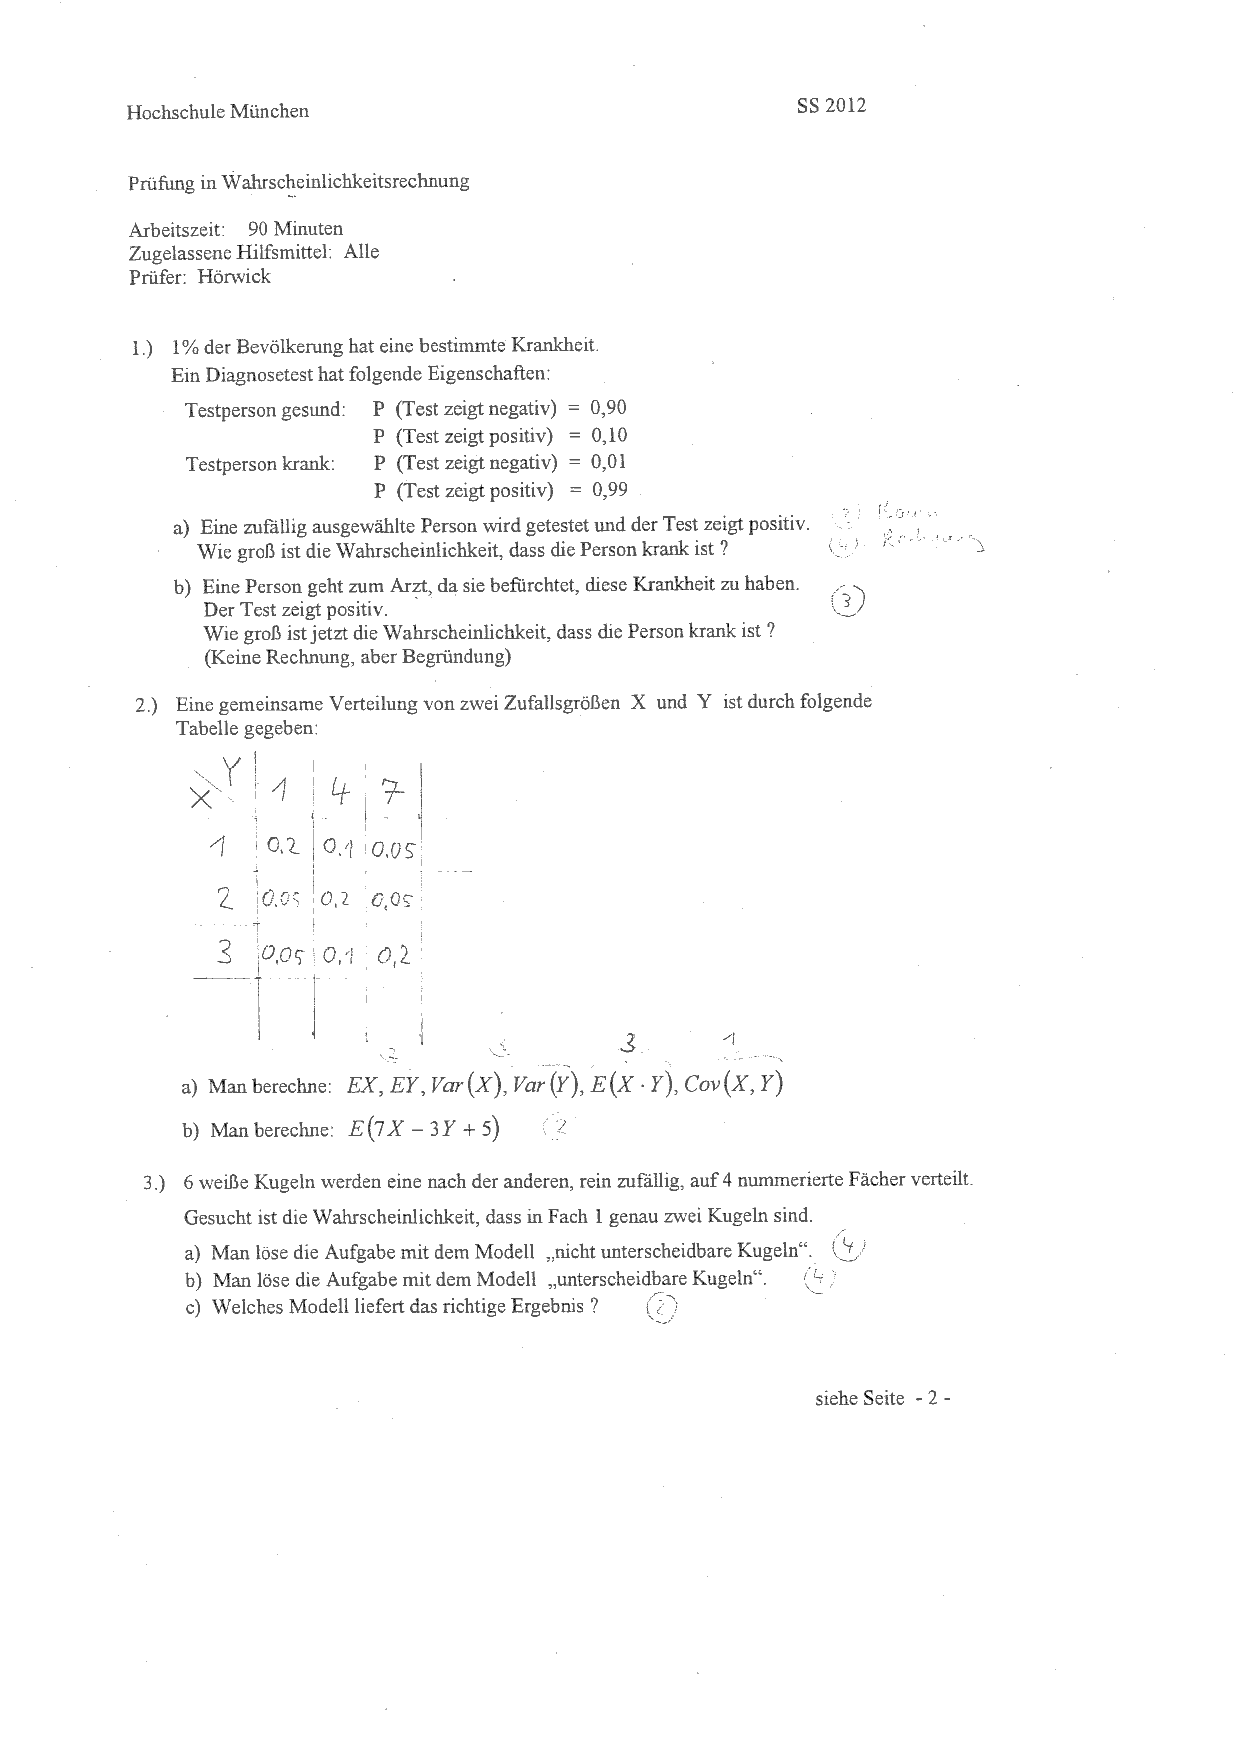
\includepdf[pages=-]{pruefungsangabe_wahrStat_ss2012}

\section{Lösung für die Prüfung SS 2012}

Lösung über die Feiertage selbst ausprobieren. Besprechung erfolgt Anfang Januar.
\renewcommand{\ldate}{2016-01-12}
% 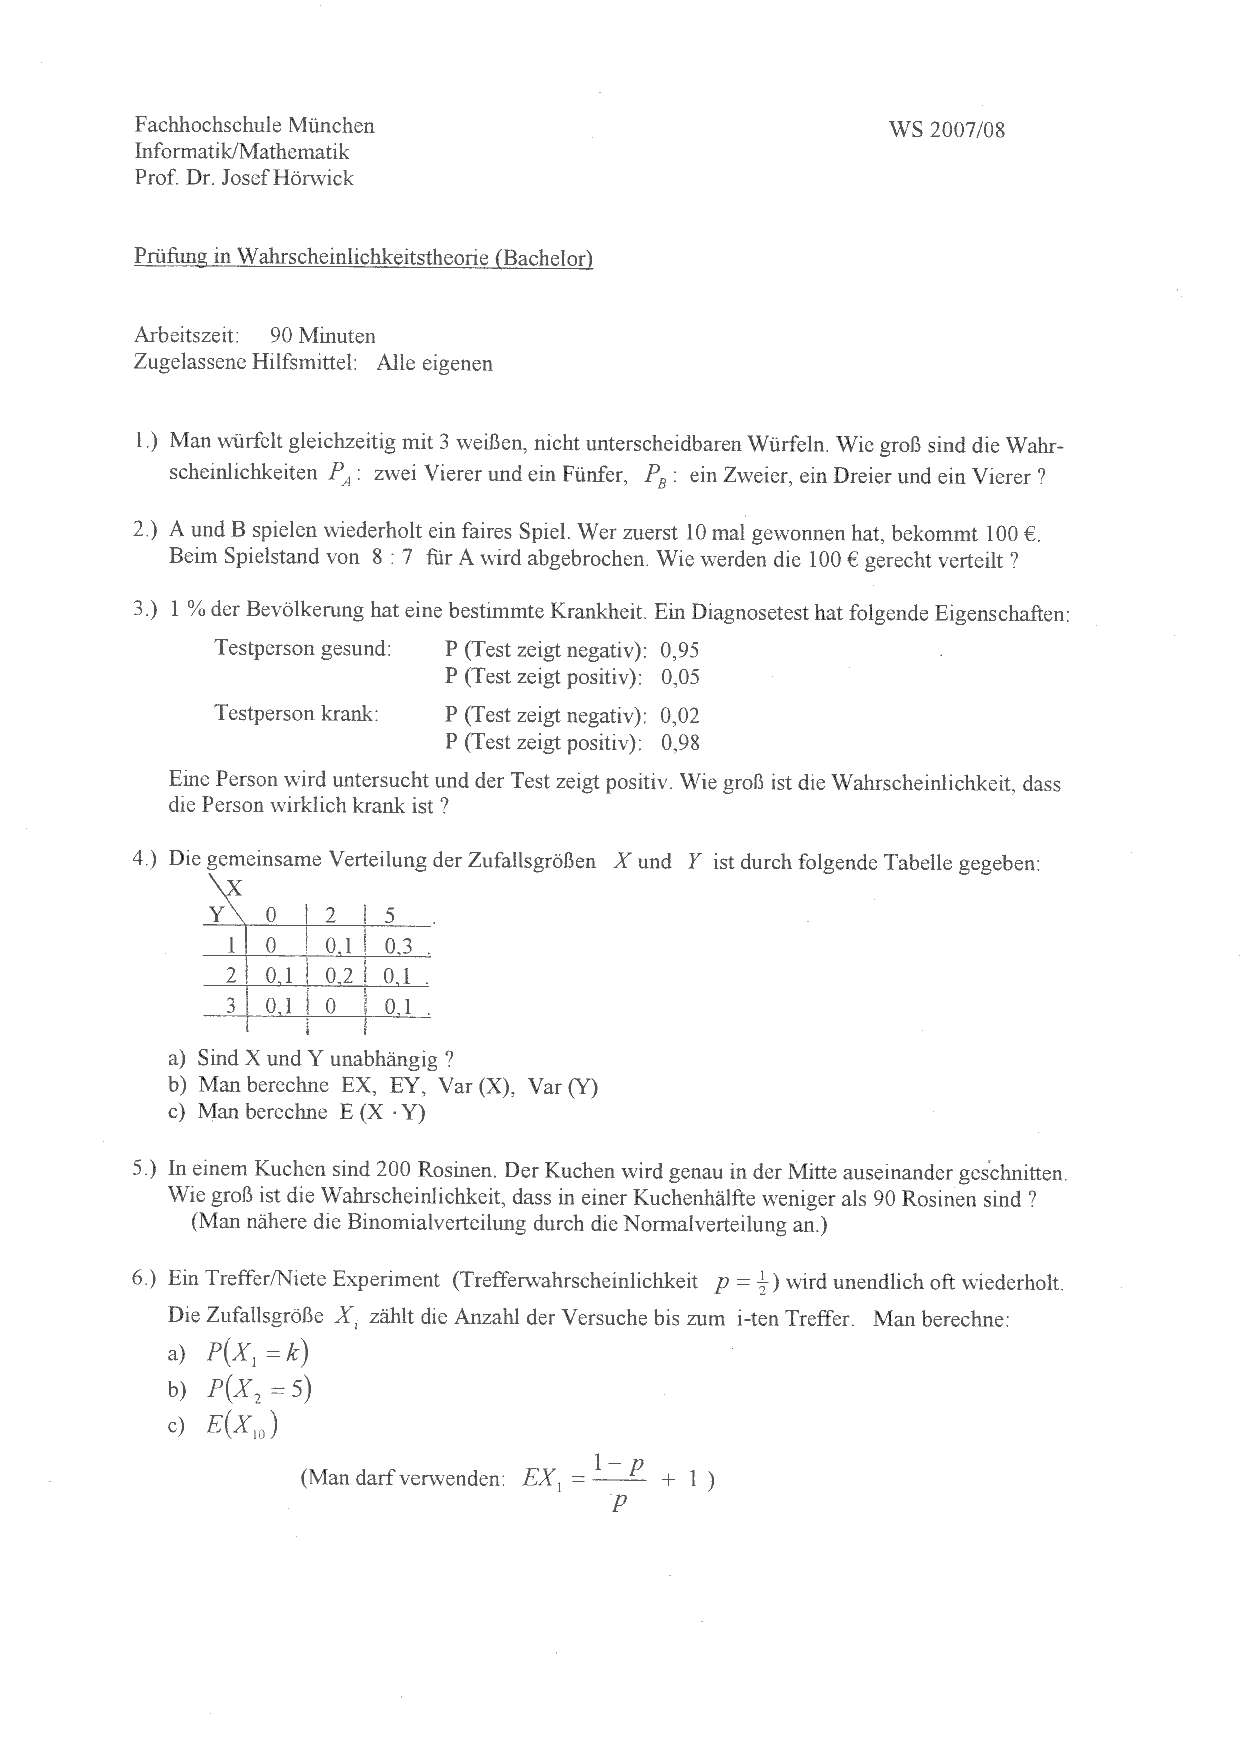
\includepdf[pages=-]{pruefungsangabe_wahrStat_ws0708}

\section{Lösung für die Prüfung WS 2007/08}

\subsection{zu 1)}
Wir stellen uns die Würfel verschiedenfarbig vor, dann ist es leichter (rot, grün, weiß). 

Alle Möglichkeiten: $ 6^3 = 216 $. Jede Möglichkeit ist gleich wahrscheinlich.

Günstige Möglichkeiten $P_A$: 

\begin{tabular}{|c|c|c|}
\hline r & g & w \\ 
\hline 5 & 4 & 4 \\ 
\hline 4 & 5 & 4 \\ 
\hline 4 & 4 & 5 \\ 
\hline 
\end{tabular}  
$\Rightarrow 3$ Möglichkeiten
$\Rightarrow P_A = \frac{3}{216} = 0.0138...$

Günstige Möglichkeiten $P_B$: 

\begin{tabular}{|c|c|c|}
\hline r & g & w \\ 
\hline 2 & 3 & 4 \\ 
\hline 2 & 4 & 3 \\ 
\hline 3 & 2 & 4 \\ 
\hline 3 & 4 & 2 \\ 
\hline 4 & 2 & 3 \\ 
\hline 4 & 3 & 2 \\ 
\hline 
\end{tabular}  
$\Rightarrow 6$ Möglichkeiten
$\Rightarrow P_A = \frac{6}{216} = 0.0277...$

\subsection{zu 2)}
Wie groß ist die Wahrscheinlichkeit, dass A beim Spielstand 8:7 gewinnt? Wir stellen uns vor, dass die beiden noch vier mal Spielen. Wir schreiben uns alle Spielausgänge hin. Diese sind gleich wahrscheinlich (halbe halbe). \color{red} A gewinnt \color{blue} B gewinnt. 

\color{red}

A A A A\\
B A A A\\
A B A A\\
A A B A\\
A A A B\\

\color{black}
Jetzt gewinnt jeder zweimal:
\color{red}

B B A A\\ 
B A B A\\
B A A B\\
A B B A\\
A B A B\\
A A B B\\
\color{black}
Jetzt gewinnt B dreimal: 
\color{blue}

A B B B\\
B A B B\\
B B A B\\
B B B A\\
B B B B\\
\color{black}
$P(\textrm{A gewinnt}) = \frac{11}{16} $ A bekommt $ 100 \textrm{ EUR} \cdot \frac{11}{16} = 68.75 \textrm{ EUR}$

\subsection{zu 3)}
Siehe Prüfung SS 2012

\subsection{zu 4)}
Siehe Prüfung SS 2012

\subsection{Exkurs: Annäherung der Binomialverteilung durch die Normalverteilung}
\profnote{Neuer Stoff für Aufgabe 5.}
Die zufallsgröße S sei $Bin(n,p)$ verteilt. Wir haben ein Treffer-Niete-Experiment mit der Trefferwahrscheinlichkeit p, das n mal wiederholt wird. S zählt die Anzahl der Treffer (0 bis n).\\

$P(S=k) = \binom n k \cdot p^k \cdot q^{n-k} $ mit $ q = 1-p, k=0,1,...,n, ES = np, Var(S)=npq $\\

Wir standardisieren S:

$ S^* = \frac{S - ES}{\sqrt{Var(S)}} $, wobei $S^*$ den Erwartungswert 0 und die Varianz 1 hat. 

$ x_j = \frac{j - np}{\sqrt{npq}}, j=0,1,...,k $\\

$ S^* $ kann die Werte $x_j$ annehmen. 

$ P (S^* = x_j) = P(S=j) $

Abstand von $x_{j+1}$ und $x_j$ ist mit $\frac{1}{\sqrt{npq}}$ immer gleich. \\

Zeichne von $S^*$ das Histogramm: Dazu zeichnen wir über $x_j$ ein Rechteck mit der Breite $\frac{1}{\sqrt{npq}}$ und Fläche $P(S^* = x_j) $.\\

Höhe des Rechtecks über $x_j$: $ \frac{1}{npq} \cdot h_j = P(S^* = x_j) = \binom n j \cdot p^j \cdot q^{n-j} $\\

% 1 \includegraphicsdeluxe{histogrammWS0708ex.jpg}{Histogramm}{So könnte das Histogramm aussehen}{fig:histogrammWS0708ex}
Man kann zeigen: Für große n nähert sich das Histogramm der Gaußschen Glockenkurve an (Abb. \ref{fig:histogrammWS0708ex}):
$ \varphi(x) = \frac{1}{\sqrt{2\pi}} \cdot exp\rbr{-\frac{x^2}{2}}$ Dabei ist $\varphi(x) $ die Dichte der Normalverteilung. 

$ \Phi(t) = \int_{-\infty}^{t} \varphi(x) dx$. $ \Phi(t)$ ist die Stammfunktion von $\varphi(x)$, kann aber nicht als Formel angegeben werden. Es gibt nur eine Tabelle. \\

Es gilt:
\begin{enumerate}
\item $ \int_{-\infty}^{\infty} \varphi(x) dx = 1$
\item $ \int_{-\infty}^{0} \varphi(x) dx = \frac{1}{2}, \varphi$ ist symmetrisch zur y-Achse.
\item $ \Phi(-t) = 1 - \Phi(t) \Rightarrow $ Wir brauchen die Tabelle nur für positive Werte. 
\end{enumerate} 

Damit kann man die Binomialverteilung durch die Normalverteilung annähern. 

S ist binomialverteilt $Bin(n,p)$

$ P(a \leq S \leq b) 
= P \rbr{\underbrace{\frac{a-np}{\sqrt{npq}}}_{u} \leq \underbrace{\frac{S-np}{\sqrt{npq}}}_{S^*} \leq \underbrace{\frac{b-np}{\sqrt{npq}}}_{v}}
= P( u\leq S^* \leq v)
\approx \int_{u}^{v} \varphi(x) dx = \Phi(v) - \Phi(u) 
$ (noch ungenau).

% 2-3 \includegraphicsdeluxe{besserWSRechtecke.jpg}{Histogramm}{Histogramm: u und v}{fig:besserWSRechtecke}
Beim ersten und letzten Rechteck fehlt eine Hälfte (Abb. \ref{fig:besserWSRechtecke}), deshalb besser: 

$P \rbr{\underbrace{\frac{a - \frac{1}{2} - np}{\sqrt{npq}}}_{u} \leq S^* \leq \underbrace{\frac{b + \frac{1}{2} - np}{\sqrt{npq}}}_{v} }$

\subsection{zu 5)}
L ist die linke Kuchenhälfte

X ist die Anzahl der Rosinen in L.

X ist binomialverteilt: $ n = 200, p=0.5 $

$ P(X < 90) + P(X > 110) $

Gegenereignis: 

$ P(90 \leq X \leq 110) $ mit $ EX = np = 200 \cdot 0.5 = 100 $ und $ Var(X) = npq = 200\cdot 0.5 \cdot 0.5 = 50 \Rightarrow $ 
$ P(90 \leq X \leq 110) 
= P\rbr{\frac{90 - 0.5 - 100}{\sqrt{50}} \leq X^* \leq \frac{110 + 0.5 - 100}{\sqrt{50}} }
= P(-1.48 \leq X^* \leq 1.48)
\approx \int_{-1.48}^{1.48} = \Phi(1.48) - \Phi(-1.48) 
= \Phi(1.48) - \underbrace{[1-\Phi(1.48)]}_{\textrm{Formel!}}
= 2 \cdot \Phi(1.48) -1 
= 2\cdot 0.93056 - 1 = $
\underline{$0.86...$}

Die gesuchte Wahrscheinlichkeit (wir haben ja das Gegenereignis ausgerechnet) ist damit $1-0.86...= 0.14$

\subsection{zu 6)}
Siehe Prüfung SS 2012


% Stichwortverzeichnis
\newpage
\renewcommand{\indexname}{Stichwortverzeichnis} % Index soll Stichwortverzeichnis heissen
\addcontentsline{toc}{section}{Stichwortverzeichnis} % Stichwortverzeichnis soll im Inhaltsverzeichnis auftauchen
\printindex % Stichwortverzeichnis endgueltig anzeigen
\end{document}